% ---------------------------------------------------------------------------
% Author guideline and sample document for EG publication using LaTeX2e input
% D.Fellner, v1.13, Nov 13, 2007

%\documentclass[draft]{egpubl}
\documentclass{egpubl}

% --- for  Annual CONFERENCE
% \ConferenceSubmission % uncomment for Conference submission
% \ConferencePaper      % uncomment for (final) Conference Paper
% \STAR                 % uncomment for STAR contribution
% \Tutorial             % uncomment for Tutorial contribution
% \ShortPresentation    % uncomment for (final) Short Conference Presentation
%
% --- for  CGF Journal
\JournalSubmission    % uncomment for submission to Computer Graphics Forum
% \JournalPaper         % uncomment for final version of Journal Paper
%
% --- for  CGF Journal: special issue
% \SpecialIssueSubmission    % uncomment for submission to Computer Graphics Forum, special issue
% \SpecialIssuePaper         % uncomment for final version of Journal Paper, special issue
%
% --- for  EG Workshop Proceedings
% \WsSubmission    % uncomment for submission to EG Workshop
% \WsPaper         % uncomment for final version of EG Workshop contribution
%
 \electronicVersion % can be used both for the printed and electronic version

% !! *please* don't change anything above
% !! unless you REALLY know what you are doing
% ------------------------------------------------------------------------

% for including postscript figures
% mind: package option 'draft' will replace PS figure by a filname within a frame
\ifpdf \usepackage[pdftex]{graphicx} \pdfcompresslevel=9
\else \usepackage[dvips]{graphicx} \fi

\PrintedOrElectronic

% prepare for electronic version of your document
\usepackage{t1enc,dfadobe}
\usepackage{multirow}
\usepackage{rotating}
\usepackage{egweblnk}
\usepackage{cite}

% For backwards compatibility to old LaTeX type font selection.
% Uncomment if your document adheres to LaTeX2e recommendations.
\let\rm=\rmfamily    \let\sf=\sffamily    \let\tt=\ttfamily
\let\it=\itshape     \let\sl=\slshape     \let\sc=\scshape
\let\bf=\bfseries
\let\vec=\mathbf
\let\mat=\mathbf
\let\set=\mathcal
\newcommand{\para}[1]{\noindent{\bf #1}}
% end of prologue


%-------------------------------------------------------------------------
%% ADDITIONAL PACKAGES AND FORMATTING COMMANDS
%-------------------------------------------------------------------------

%% AMS mathematics packages
\usepackage{amsfonts,amsmath,amssymb}

% text colors
\usepackage[usenames,dvipsnames]{color}

% This package allows multi-line comments.
\usepackage{verbatim}

%% Symbols
\newcommand{\ba}{\mathbf{a}}
\newcommand{\bb}{\mathbf{b}}
\newcommand{\bc}{\mathbf{c}}
\newcommand{\bd}{\mathbf{d}}
\newcommand{\be}{\mathbf{e}}
\newcommand{\bff}{\mathbf{f}}
\newcommand{\bg}{\mathbf{g}}
\newcommand{\bh}{\mathbf{h}}
\newcommand{\bi}{\mathbf{i}}
\newcommand{\bj}{\mathbf{j}}
\newcommand{\bk}{\mathbf{k}}
\newcommand{\bl}{\mathbf{l}}
\newcommand{\bm}{\mathbf{m}}
\newcommand{\bn}{\mathbf{n}}
\newcommand{\bo}{\mathbf{o}}
\newcommand{\bp}{\mathbf{p}}
\newcommand{\bq}{\mathbf{q}}
\newcommand{\br}{\mathbf{r}}
\newcommand{\bs}{\mathbf{s}}
\newcommand{\bt}{\mathbf{t}}
\newcommand{\bu}{\mathbf{u}}
\newcommand{\bv}{\mathbf{v}}
\newcommand{\bw}{\mathbf{w}}
\newcommand{\bx}{\mathbf{x}}
\newcommand{\by}{\mathbf{y}}
\newcommand{\bz}{\mathbf{z}}
\newcommand{\bA}{\mathbf{A}}
\newcommand{\bB}{\mathbf{B}}
\newcommand{\bC}{\mathbf{C}}
\newcommand{\bD}{\mathbf{D}}
\newcommand{\bE}{\mathbf{E}}
\newcommand{\bF}{\mathbf{F}}
\newcommand{\bG}{\mathbf{G}}
\newcommand{\bH}{\mathbf{H}}
\newcommand{\bI}{\mathbf{I}}
\newcommand{\bJ}{\mathbf{J}}
\newcommand{\bK}{\mathbf{K}}
\newcommand{\bL}{\mathbf{L}}
\newcommand{\bM}{\mathbf{M}}
\newcommand{\bN}{\mathbf{N}}
\newcommand{\bO}{\mathbf{O}}
\newcommand{\bP}{\mathbf{P}}
\newcommand{\bQ}{\mathbf{Q}}
\newcommand{\bR}{\mathbf{R}}
\newcommand{\bS}{\mathbf{S}}
\newcommand{\bT}{\mathbf{T}}
\newcommand{\bU}{\mathbf{U}}
\newcommand{\bV}{\mathbf{V}}
\newcommand{\bW}{\mathbf{W}}
\newcommand{\bX}{\mathbf{X}}
\newcommand{\bY}{\mathbf{Y}}
\newcommand{\bZ}{\mathbf{Z}}
\newcommand{\balpha}{\mbox{\boldmath$\alpha$}}
\newcommand{\bgamma}{\mbox{\boldmath$\gamma$}}
\newcommand{\bGamma}{\mbox{\boldmath$\Gamma$}}
\newcommand{\bmu}{\mbox{\boldmath$\mu$}}
\newcommand{\bphi}{\mbox{\boldmath$\phi$}}
\newcommand{\bksi}{\mbox{\boldmath$\xi$}}
\newcommand{\bPhi}{\mbox{\boldmath$\Phi$}}
\newcommand{\bSigma}{\mbox{\boldmath$\Sigma$}}
\newcommand{\bsigma}{\mbox{\boldmath$\sigma$}}
\newcommand{\btheta}{\mbox{\boldmath$\theta$}}

\newcommand{\Ex}{\mathbb{E}}


\newcommand{\mL}{\mathcal{L}}
\newcommand{\mN}{\mathcal{N}}
\newcommand{\mU}{\mathcal{U}}
\newcommand{\mC}{\mathcal{C}}
\newcommand{\mS}{\mathcal{S}}
\newcommand{\mR}{\mathcal{R}}
\newcommand{\mD}{\mathcal{D}}
\newcommand{\mT}{\mathcal{T}}
\newcommand{\mSl}{\mathcal{S}_l}
\newcommand{\mNl}{\mathcal{N}_l}
\newcommand{\mDll}{\mathcal{D}_{l,l'}}

\def\ll{{\mathcal{\ell}}}

\def\A{{\cal A}}
\def\B{{\cal B}}
\def\C{{\cal C}}
\def\D{{\cal D}}
\def\E{{\cal E}}
\def\F{{\cal F}}
\def\G{{\cal G}}
\def\H{{\cal H}}
\def\I{{\cal I}}
\def\J{{\cal J}}
\def\K{{\cal K}}
\def\L{{\cal L}}
\def\M{{\cal M}}
\def\N{{\cal N}}
\def\O{{\cal O}}
\def\P{{\cal P}}
\def\Q{{\cal Q}}
\def\R{{\cal R}}
\def\S{{\cal S}}
\def\T{{\cal T}}
\def\U{{\cal U}}
\def\V{{\cal V}}
\def\W{{\cal W}}
\def\X{{\cal X}}
\def\Y{{\cal Y}}
\def\Z{{\cal Z}}
\def\Re{{\mathbb R}}
\def\Cx{{\mathbb C}}
\def\Ze{{\mathbb Z}}
\def\Na{{\mathbb N}}
\def\Wh{{\mathbb W}}
\def\bd{\partial}
\def\ud{\mathrm{d}}
\def\eps{\varepsilon}
\def\dist{\textrm{dist}}
\DeclareMathOperator*{\argmax}{arg\,max}


%% Inlined comments
\def\kai#1{\textcolor{green}{({Kai says: }{#1})}}
\def\peter#1{\textcolor{red}{({Peter says: }{#1})}}
\def\vova#1{\textcolor{blue}{({Vova says: }{#1})}}
\def\vangelis#1{\textcolor{magenta}{({Vangelis says: }{#1})}}

\def\rev#1{\textcolor{black}{#1}}

\def\fix#1{\textcolor{black}{#1}}


%\renewcommand\floatpagefraction{.9}
%\renewcommand\topfraction{.9}
%\renewcommand\bottomfraction{.9}
%\renewcommand\textfraction{.1}
%\setcounter{totalnumber}{50}
%\setcounter{topnumber}{50}
%\setcounter{bottomnumber}{50}
\linespread{0.94}
\addtolength{\textfloatsep}{-0.1in}
%\renewcommand{\topfraction}{1.00}
%\clubpenalty=10000
%\widowpenalty=10000




% ---------------------------------------------------------------------
% EG author guidelines plus sample file for EG publication using LaTeX2e input
% D.Fellner, v1.16, Jan 21, 2009


\title[Data-Driven Shape Analysis and Processing]%
      {Data-Driven Shape Analysis and Processing}

% for anonymous conference submission please enter your SUBMISSION ID
% instead of the author's name (and leave the affiliation blank) !!
\author[K. Xu \& V. Kim \& Q. Huang \& E. Kalogerakis]
       %{Kai Xu\thanks{Corresponding author: kevin.kai.xu@gmail.com}$^{1,2}$
	   {Kai Xu$^{1,2}$
        \quad Vladimir G. Kim$^{3,4}$
        \quad Qixing Huang$^{5}$
        \quad Evangelos Kalogerakis$^{6}$
        \\
% For Computer Graphics Forum: Please use the abbreviation of your first name.
         $^1$ National University of Defense Technology \quad
         $^2$ Shenzhen VisuCA Key Lab / SIAT \quad
         $^3$ Stanford University \quad \\
         $^4$ Adobe Research \quad
         $^5$ Toyota Technological Institute at Chicago \quad
         $^6$ University of Massachusetts Amherst
%             with different affiliations
       }

% ------------------------------------------------------------------------

% if the Editors-in-Chief have given you the data, you may uncomment
% the following five lines and insert it here
%
% \volume{27}   % the volume in which the issue will be published;
% \issue{1}     % the issue number of the publication
% \pStartPage{1}      % set starting page


%-------------------------------------------------------------------------
\begin{document}

\maketitle

\begin{abstract}

Data-driven methods serve an increasingly important role in discovering geometric, structural, and semantic relationships between shapes. 
In contrast to traditional approaches that process shapes in isolation of each other, data-driven methods aggregate information from 3D model collections to improve the analysis, modeling and editing of shapes.
\rev{Data-driven methods are also able to learn computational models that reason about properties and relationships of shapes without relying on hard-coded rules or explicitly programmed instructions.} 
Through reviewing the literature, we provide an overview of the main concepts and components of these methods, as well as discuss their application to classification, segmentation, matching, reconstruction, modeling and exploration, as well as scene analysis and synthesis.  
We conclude our report with ideas that can inspire future research in data-driven shape analysis and processing. 

\begin{classification} % according to http://www.acm.org/class/1998/
\CCScat{Computer Graphics}{I.3.3}{Picture/Image Generation}{Line and curve generation}
\end{classification}

\end{abstract}


%-------------------------------------------------------------------------

\section{Introduction}
\label{sec:intro}

%{\em
%``The goal is to turn data into information, and information into insight.''}
%\vspace{-5pt}
%\begin{flushright}
%--- Carly Fiorina
%\end{flushright}

%Recent interest on geometry processing has been moving towards high-level understanding and intelligent processing of
%three dimensional shapes, with a general goal of discovering patterns about their compositions and structures,
%and relating structures with semantic meanings and functionalities.
%This momentum gives rise to the recent topic of structure-aware geometry processing~\cite{Mitra:2014:SASP}.
%Shape structure implies human knowledge about 3D shapes in terms of part configurations.
%Thus, a natural approach to structural shape analysis and structure-aware shape processing is knowledge-driven,
%where structure is extracted, interpreted and represented with domain-specific knowledge incorporated.
%Examples are like minima-rule-based heuristics for shape segmentation~\cite{Shamir:2008:SMS}, procedural models~\cite{Muller:2006:PMB}
%and rule-based generative models~\cite{Merrell:2011:IFL} for 3D shape modeling.

\rev{As the availability of 3D data increases, due to the developments in both 3D sensing technology as well as 3D modeling software, data-driven approaches become increasingly applicable and useful to 3D shape processing.  In contrast to traditional approaches~\cite{LevyZhang:2011:EGP}, data-driven methods look beyond single objects, instead analyzing sets of shapes jointly to extract meaningful mappings and correlations between them. In addition, these methods are able to learn from data computational models that effectively reason about properties and relationships of shapes without relying on hard-coded rules or explicitly programmed instructions. Leveraging shared information across multiple objects, data-driven methods are able to facilitate high-level shape understanding through discovering geometric and structural patterns among collections of shapes, patterns which serve as strong priors in various geometry processing applications.}

The idea of utilizing data to support geometry processing has been exploited and practiced for many years. However, most existing works based on this idea are confined to the example-based paradigm, mostly leveraging only one core concept of data-driven techniques -- \emph{information transfer}. Typically, the input to these problems includes one or multiple exemplar shapes with some prescribed or precomputed information of interest, and a target shape that needs to be analyzed or processed. These techniques usually establish a \emph{correlation} between the source and the target shapes and transfer the interesting information from the source to the target. The applications of such approaches include a variety of methods in shape analysis (e.g.~\cite{Schaefer:2007:EBS}) and shape synthesis (e.g.~\cite{Merrell:2007:EBM,Ma:2014:ADS}).

As the availability of 3D data increases, several new concepts in data-driven methods are emerging, opening space for new developments in shape analysis and content creation.
\emph{First}, the rich variability of 3D content in existing shape repositories makes it possible to directly reuse the shapes or parts for constructing new 3D models~\cite{Funkhouser:2004:MBE}. \emph{Content reuse} for 3D modeling is perhaps the most straightforward application of big 3D geometric data, providing a promising approach to address the challenging 3D content creation problem.
%
\emph{Second}, high-level shape understanding can benefit from co-analyzing collections of shapes. Several analysis tools demonstrate that shape analysis is more reliable if it is supported by observing certain attributes across a set of semantically related shapes instead of just focusing on a single object. \emph{Co-analysis} requires a critical step of finding correlations between multiple shapes in the input set, which is substantially different from building pair-wise correlation. \rev{A key concept to co-analysis is the \emph{consistency} of the correlations across the entire set, which has both semantic~\cite{Kalogerakis:2010:LMS,Sidi:2011:CS,Wang:2012:ACS} and mathematical~\cite{Huang:2013:SDP} justifications.}
%
\fix{
\emph{Third},
aside from analyzing patterns from a set of shapes,
it is also possible to endorse a subset of the shapes with some semantic information (e.g., part labeling), which can be propogated to the other shapes through learned mappings.
This information propogation evolves the concept of \emph{knowledge transfer} between shapes.
}

\begin{figure}[t!]
\centering
    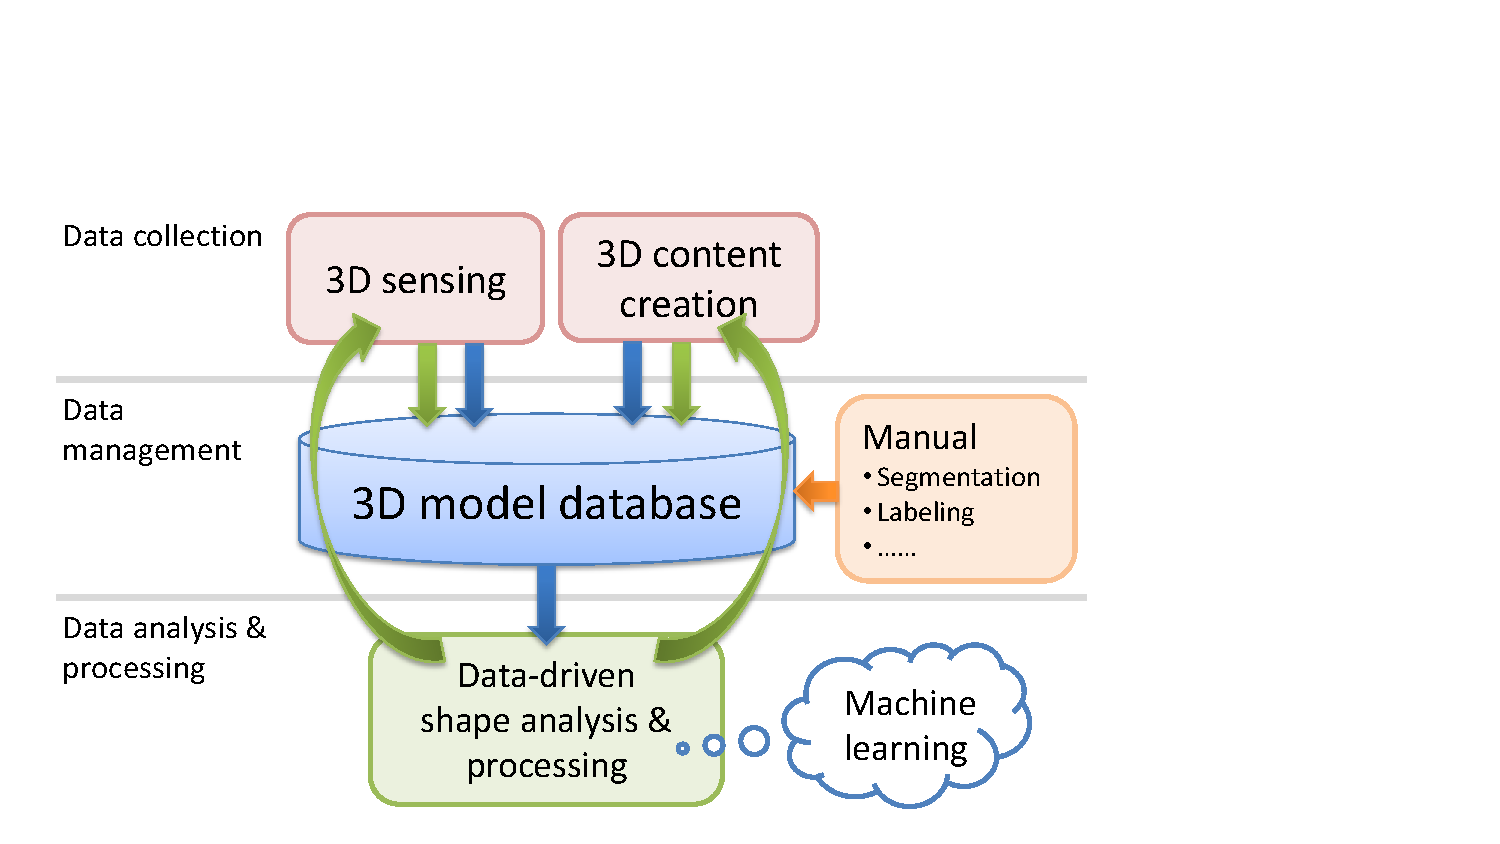
\includegraphics[width=0.99\linewidth]{fig/img/teaser.pdf}
    %\vspace{-.2cm}
    \caption{\rev{Data-driven shape processing and modeling provides a promising solution to the development of ``big 3D data''.
    The two major ways of 3D data generation, 3D sensing and 3D content creation, populate 3D databases with fast growing amount of 3D models.
    The database models are sparsely augmented with manual segmentation and labeling, as well as reasonably
    organized, to support data-driven shape analysis and processing, based on, e.g., machine learning techniques.
    The learned knowledge can in turn support efficient 3D reconstruction and 3D content creation, during which
    the knowledge can be transferred to the newly generated data.
    Such 3D data with semantic information can be included into the database to enrich it and facilitate further data-driven applications.}}
    \label{fig:teaser}
\end{figure}



\paragraph*{Relation to knowledge-driven shape processing.}
Prior to the emergence of data-driven techniques, high-level shape understanding and modeling was usually achieved with knowledge-driven methods.
In the knowledge-driven paradigm, geometric and structural patterns are extracted and interpreted with the help of explicit rules or hand-crafted parameters.
Such examples include heuristics-based shape segmentation~\cite{Shamir:2008:SMS} and procedural shape modeling~\cite{Muller:2006:PMB}.
Although these approaches have certain empirical success, they exhibit several inherent limitations. First, it is extremely difficult to hard-code explicit rules and heuristics that can handle the enormous geometric and structural variability of 3D shapes and scenes in general.
\fix{As a result, knowledge-driven approaches are often hard to generalize well to large and diverse shape collections.}
Another issue is that non-experts find it difficult to interact with knowledge-driven techniques that require as input ``low-level'' geometric parameters or instructions.
%The main problem is that converting human knowledge into hand-crafted rules, heuristics and manually tuned models or algorithms is unlikely to handle the enormous geometric and structural variability of 3D shapes.
%can be used to capture human understanding of 3D shapes.
%Another problem is that human experience and judgment are usually formed with limited observations, which usually does not generalize well to big data.
%This problem becomes especially notable in 3D shapes, among objects that possess significant structural variations.

\rev{In contrast to knowledge driven methods, data-driven techniques learn representations and parameters from data. They usually do not depend on hard-coded prior knowledge, and consequently do not rely on hand-crafted parameters, making these techniques more data-adaptive and thus lead to significantly improved performance in many practical settings.}
The success of data-driven approaches, backed by machine learning techniques, heavily relies on the accessibility of large data collections.
We have witnessed the successful performance improvement of machine learning algorithms by increasing the training set size~\cite{Banko:2001:MPA}. In light of this, the recent developments in 3D modeling tools and acquisition techniques for 3D geometry, as well as availability of large repositories of 3D shapes (e.g., Trimble 3D Warehouse, Yobi3D , etc.), offer great opportunities for developing data-driven approaches for 3D shape analysis and processing.
% and stimulate this direction of research.


\paragraph*{Relation to structure-aware shape processing.}
This report is closely related to the recent survey on ``structure-aware shape processing'' by Mitra and co-workers~\cite{Mitra:2014:SASP},
which concentrates on techniques for structural analysis of 3D shapes, as well as high-level shape processing guided by structure-preservation.
In that survey, shape structure is defined as the arrangement and relations between shape parts, which is analyzed through identifying shape parts, part parameters, and part relations. Each of the three can be determined through manual assignment, predefined model fitting and data-driven learning.

In contrast, our report takes a very different perspective---we focus on how the increasing availability of geometric data has changed the field of shape analysis and processing. In particular, we want to highlight several key distinctions:
\emph{First}, data-driven shape processing goes beyond structure analysis.
For example, leveraging large shape collections may benefit a wider variety of problems in shape understanding and processing, such as parametric modeling of shape space~\cite{Allen:2003:SHB}, hypothesis generation for object and scene understanding~\cite{Zia:2013:DR,Satkin:2012:DDS}, and information transfer between multi-modal data~\cite{Wang:2013:PAS,Su:2014:EID}. Data-driven shape processing may also exploit the data-centered techniques in machine learning such as sparse representation~\cite{Ren:2013:HSC} and feature learning~\cite{Hinton:DBN:2006,Bengio:2009:LDA,Yu:FLI:2010,Krizhevsky:ICDL:2012}, which are not pre-conditioned on any domain-specific or structural prior beyond raw data.
%
\emph{Second}, even within the realm of structure-aware shape processing, data-driven approaches are arguably becoming dominant due to their theoretical and practical advantages, as well as the availability of large shape repositories and recent developments in machine learning.

\begin{figure*}[t!]
\centering
    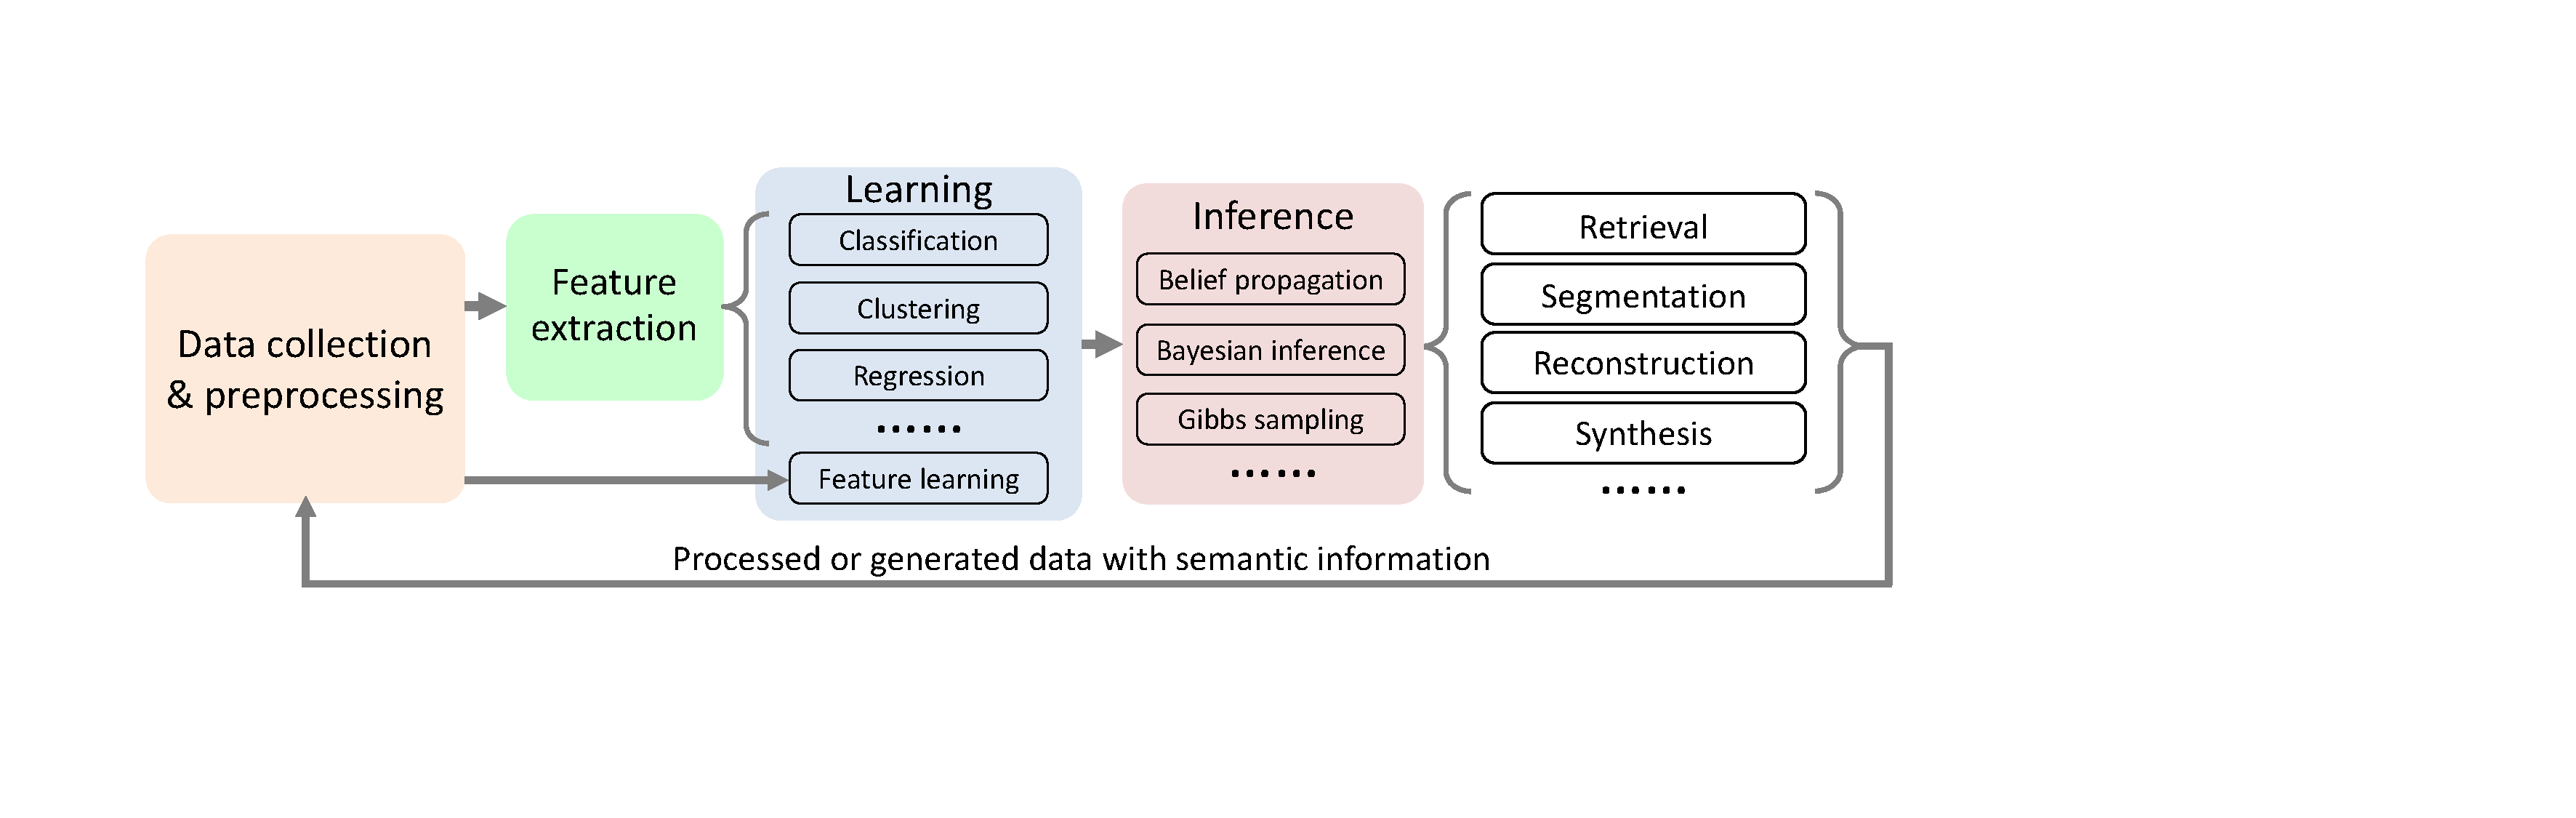
\includegraphics[width=0.9\textwidth]{fig/img/overview.pdf}
    %\vspace{-.4cm}
    \caption{
\rev{The general pipeline of data-driven geometry processing contains four major stages: data collection and preprocessing, feature extraction (or feature learning),
learning and inference. The inference supports many applications which would produce new shapes or scenes through reconstruction modeling or synthesis.
These new data, typically possessing labels for shapes or parts, can be used to enrich the input datasets and enhance the learning tasks in future, forming a data-driven geometry processing loop.}}
    \label{fig:overview}
\end{figure*}



\paragraph*{Vision and motivation.}
\rev{With the emergence of ``big data'', many scientific disciplines have shifted their focus to data-driven techniques. Although 3D geometry data is still far from being as ubiquitous as some other data formats (e.g., photographs), the rapidly growing number of 3D models, the recent developments in fusing 2D and 3D data, and the invention of commodity depth sensors,
%which opens door to low-cost universal acquisition of 3D data associated with 2D images,
have made the era of ``big 3D data'' more promising than ever.}
%The invention of commodity RGB-D camera has opened the door to low-cost, universal acquisition of 3D data, and brought new possibilities for connecting 2D and 3D data. %The connection of 2D and 3D data will provide much more enriched data sources for data-driven methods.
%Furthermore, we expect geometric data to serve as a media that connects multiple modalities.  For example, RGB-D cameras naturally relate images (i.e., the appearance) to shape geometry, or annotated 3D shapes relate geometries to human language.
%
At the same time, we expect data-driven approaches to take one of the leading roles in the reconstruction and understanding of acquired 3D data, as well as the synthesis of new shapes.
%These newly generated data typically comes with rich semantic information produced by data-driven inference, which will enhance exiting shape collections with both reusable content and training labels.
Data-driven geometry processing will close the loop starting from acquisition, analysis, and processing all the way to the generation of 3D shapes (see Figure~\ref{fig:teaser}), and will be a key tool for manipulating big visual data.

Recent years have witnessed a rapid development of data-driven geometry processing algorithms, both in the computer graphics and computer vision communities. Given the research efforts and wide interests in the subject, we believe many researchers would benefit from a comprehensive and systematic survey. \rev{We also hope such a survey can stimulate new theories, problems, and applications.} 

\paragraph*{Organization.}
This survey is organized as follows. Section~\ref{sec:overview} gives a high-level overview of data-driven approaches and classifies data-driven methods with respect to their application domains. This section also provides two representative examples for the readers to understand the general work-flow of data-driven geometry processing. The sections following survey the various data-driven shape processing problems in detail, and try to correlate the different methods through comparisons in various aspects. Finally, we conclude our survey by discussing a few key problems involved in designing a data-driven
method for shape processing, listing a set of open challenges in this direction, as well as providing a vision on future research.

\paragraph*{Accompanying online resources.}
In order to assist the reader in learning and leveraging the basic algorithms, we provide an online wikipage~\cite{Wikipage}, which collects tools and source code, together with benchmark data for typical problems and applications of data-driven shape processing. This page will also maintain links and data mining tools for obtaining large data collections of shapes and scenes. This website could serve as a starting point for those who are conducting research in this direction. We also expect it to benefit a wide spectrum of researchers from related fields.




\section{Overview}
\label{sec:overview}

In this section, we provide a high-level overview of the main components and steps of data-driven approaches for processing 3D shapes and scenes. Although the pipeline of these methods vary significantly depending on their particular applications and goals, a number of components tend to be common: the input data collection and processing, data representations and feature extraction, as well as learning and inference. \emph{Representation, learning and inference} are critical components of machine learning approaches in general \cite{Koller:2009:PGM}. In the case of shape and scene processing, each of these components poses several interesting and unique problems when dealing with 3D geometric data. These problems have greatly motivated the research on data-driven geometry processing, and in turn have brought new challenges to the computer vision and machine learning communities, as reflected by the increased interest in 3D visual data from these fields. Below, we discuss particular characteristics and challenges of data-driven 3D shape and scene processing algorithms.
\rev{Figure~\ref{fig:overview} provides a schematic overview of the most common components of these algorithms.}

\begin{figure*}[t!]
\centering
    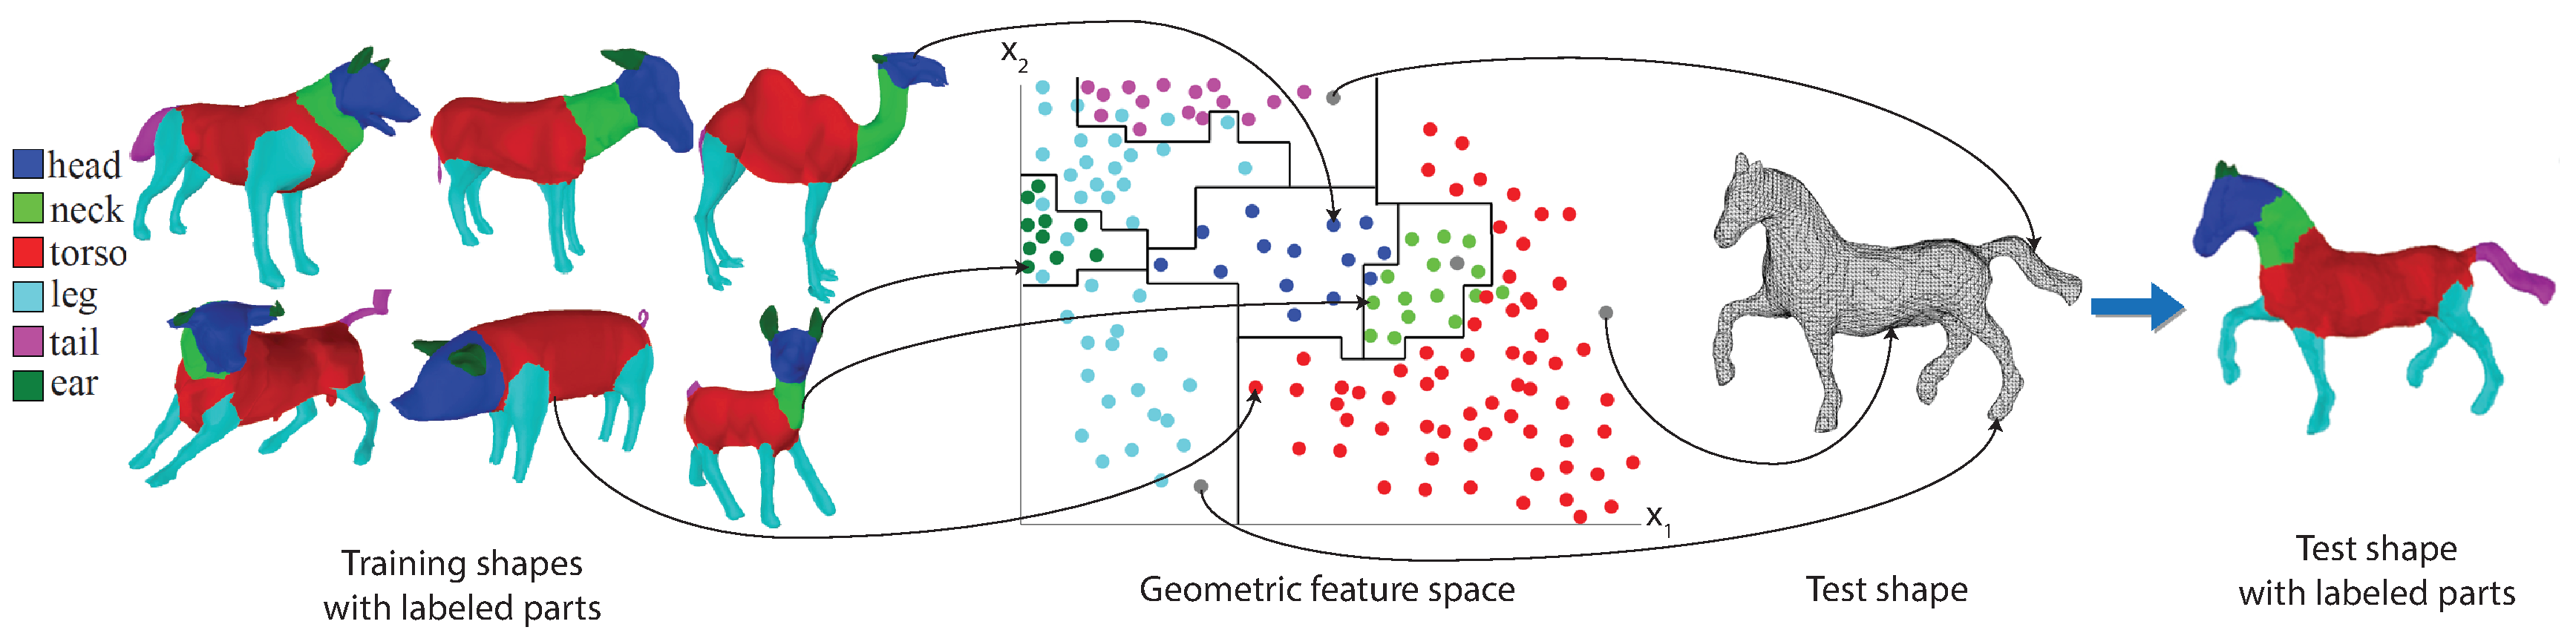
\includegraphics[width=1.0\textwidth]{fig/img/overview_seg.pdf}
    %\vspace{-.5cm}
    \caption{
Pipeline of a supervised segmentation algorithm \cite{Kalogerakis:2010:LMS}. Given a set of shapes with labeled parts, the points of each shape are embedded in a common feature space based on their local geometric descriptors (a color is assigned to points depending on their given part label). A classifier is learned to split the feature space into regions corresponding to each part label. Given a test shape, its points (shown in grey) are first embedded in the same space. Then part labels are inferred for all its points based on the learned classifier and an underlying structured probabilistic model (Section \ref{sec:segmentation}).
}
\label{fig:overview_seg}
\end{figure*}



\subsection{3D data collection}

\para{Shape representation.} A main component of data-driven approaches for shape and scene processing is data collection, where the goal is acquire a number of 3D shapes and scenes depending on the application. When shapes and scenes are captured with scanners or depth sensors, their initial representation is in the form of \emph{range data} or \emph{unorganized point clouds}. Several data-driven methods for reconstruction, segmentation and recognition directly work on these representations and do not require any further processing. On the other hand, online repositories, such as the Trimble 3D Warehouse, contain millions of shapes and scenes that are represented as \emph{polygon meshes}. A large number of data-driven techniques are designed to handle complete shapes in the form of polygon meshes created by 3D modeling tools or re-constructed from point clouds. Choosing which representation to use depends on the application. For example, data-driven reconstruction techniques aim for generating complete shapes and scenes from noisy point clouds with missing data. The reconstructed shapes can then be processed with other data-driven methods for categorization, segmentation, matching and so on. Developing methods that can handle any 3D data representation, as well as jointly reconstructing and analyzing shapes is a potential direction for future research we discuss in Section \ref{sec:conclusion}.

When polygon meshes are used as the input representation, an important aspect to consider is whether and how data-driven methods will deal with possible ``defects'', such as non-manifold and non-orientable sets of polygons, inverted faces, isolated elements, self-intersections, holes and topological noise. The vast majority of meshes available in online repositories have these problems. Although there is a number of mesh repairing tools (see \cite{Campen:PGP:2012} for a survey), they may not handle all different types of ``defects'', and can take a significant amount of time to process each shape in a large dataset. To avoid the issues caused by these ``defects'', some data-driven methods uniformly sample the input meshes and work on the resulting point-based representation instead (e.g., \cite{Chaudhuri:2011:prabm,Kim:2013:lpt}).

\paragraph*{Datasets.} Although it is desirable to develop data-driven methods that can learn from a handful of training shapes or scenes, this is generally a challenging problem in machine learning \cite{Fei:OSL:2006}. Several data-driven methods in computer vision have been particularly successful due to the use of very large datasets that can reach the size of several millions of images \cite{Torralba:2008:MTI}. In contrast, data-driven approaches for 3D shape and scene processing approaches have mostly relied on datasets that reach the order of a few thousands so far (e.g., Princeton Shape Benchmark \cite{Shilane:2004:TPS}, or datasets collected from the web \cite{Kim:2013:lpt}). Online repositories contain large amount of shapes, which can lead to the development of methods that will leverage datasets that are orders of magnitudes larger than the ones currently used.
%
\fix{One significant example is the recently available ShapeNet~\cite{Shapenet}, which provides a richly-annotated, large-scale dataset of 3D shapes.
Similar to ImageNet, a well-known image database in the computer vision community, ShapeNet is organized based on the WordNet hierarchy.
It has indexed about 3 million models, out of which 220 thousand models are classified into 3,135 WordNet synsets (a synset refers to a meaningful concept in WordNet).}

Another possibility is to develop synthetic datasets. A notable example is the pose and part recognition algorithm used in Microsoft's Kinect that relies on 500K synthesized shapes of human bodies in different poses \cite{Shotton:2011:RLH}. In general, large datasets are important to capture the enormous 3D shape and scene variability, and can significantly increase the predictive performance and usability of learning methods. A more comprehensive summary of existing online data collections can be found on our wikipage~\cite{Wikipage}.


\subsection{3D data processing and feature representation}
It is common to perform some additional processing on the input representations of shapes and scenes before executing the main learning step. The reason is that the input representations of 3D shapes and scenes can have different resolutions (e.g., number of points or faces), scale, orientation, and structure. In other words, the input shapes and scenes do not initially have any type of common parameterization or alignment. This is significantly different from other domains, such as natural language processing or vision, where text or image datasets frequently come with a common parameterization beforehand (e.g., images with the same number of pixels and objects of consistent orientation).

To achieve a common parameterization of the input shapes and scenes, one popular approach is to embed them in a \emph{common geometric feature space}. For this purpose a variety of shape descriptors have been developed. These descriptors can be classified into two main categories: \emph{global shape descriptors} that convert each shape to a feature vector,  and \emph{local shape descriptors} that convert each point to a feature vector. Examples of global shape descriptors are Extended Gaussian Images \cite{Horn:1984:EGI}, 3D shape histograms \cite{Ankerst:1999:3dsh,Chaudhuri:2010:DDS}, spherical functions \cite{Saupe:2001:MRS}, lightfield descriptors \cite{Chen:2003:ovsb}, shape distributions \cite{Osada:2002:sd}, symmetry descriptors \cite{Kazhdan:2004:SD3D}, spherical harmonics \cite{Kazhdan:2003:RISH}, 3D Zernicke moments \cite{Novotni:2003:3DZD}, and bags-of-words created out of local descriptors \cite{Bronstein:2011:SGGW}. Local shape descriptors include surface curvature, PCA descriptors, local shape diameter \cite{Shapira:2008:SDF}, shape contexts \cite{Belongie:2002:SMO,Kalogerakis:2010:LMS,Kokkinos:2012:ISC}, spin images \cite{Johnson:1999:USI}, geodesic distance features \cite{Zhang:2005:FSP}, heat-kernel descriptors \cite{Bronstein:2011:SGGW}, and depth features \cite{Shotton:2011:RLH}. Global shape descriptors are particularly useful for shape classification, retrieval and organization. Local shape descriptors are useful for partial shape matching, segmentation, and point correspondence estimation. Before using any type of global or local descriptor, it is important to consider whether the descriptor will be invariant to different shape orientations, scales, or poses. In the presence of noise and irregular mesh tessellations, it is important to robustly estimate local descriptors, since surface derivatives are particularly susceptible to surface and sampling noise \cite{Kalogerakis:2007:RSE}. It is also possible to use several different descriptors as input, and let the learning step decide which ones are more relevant for each class of shapes \cite{Kalogerakis:2010:LMS}.

\fix{
A different approach, which has attracted large attention in the computer vision community, is to avoid manually engineered features and instead directly learn features them from raw data. This approach has been enlightened by the recent developments in deep learning~\cite{Bengio:2009:LDA,Yu:FLI:2010}, and in particular Convolutional Neural Networks (CNNs) \cite{Krizhevsky:ICDL:2012,Szegedy:GDC:2015}.
A number of deep learning architectures have been recently proposed to learn 3D shape and scene descriptors, operating on either voxel-based representations \cite{Wu:3SN:2015}, view-based projections \cite{Su:MCN:2015,Xie:PFL:2015}, spectral representations \cite{Boscaini:2015:LCS}, or RGB-D data ~\cite{Socher:2012:CRD,Blum:2012:LFD,Lai:2013:UFL,Bo:2014:LHS}.}

Instead of embedding shapes in a common geometric feature space, several methods instead try to directly align shapes in Euclidean space. We refer the reader to the survey on dynamic geometry processing for a tutorial on rigid and non-rigid registration techniques \cite{Chang:DGP:2012}. An interesting extension of these techniques is to include the alignment process in the learning step of data-driven methods, since it is inter-dependent with other shape analysis tasks such as shape segmentation and correspondences \cite{Kim:2013:lpt}.

Some data-driven methods require additional processing steps on the input. For example, learning deformation handles or fully generative models of shapes usually rely on segmenting the input shapes into parts with automatic algorithms \cite{Huang:2011:JSS,Sidi:2011:CS} and representing these parts with surface abstractions \cite{Yumer:2012:CSC} or descriptors \cite{Kalogerakis:2012:PMC}. To decrease the amount of computation required during learning, it is also common to represent the shapes as a set of patches (super-faces) \cite{Huang:2011:JSS} inspired by the computation of super-pixels in image segmentation.

\subsection{Learning and Inference}
The processed representations of shapes and scenes are used to perform learning and inference for a variety of applications: shape classification, segmentation, matching, reconstruction, modeling, synthesis, and scene analysis. The learning procedures significantly vary depending on the application, thus we discuss them individually in each of the following sections on these applications. As a common theme, learning is viewed as an \emph{optimization} problem that runs on a set of variables representing geometric, structural, semantic or functional properties of shapes and scenes. There is usually a single or multiple objective (or loss) functions for quantifying preferences for different models or patterns governing the 3D data. After learning a model from the training data, inference procedures are used to predict values of variables for new shapes or scenes. Again, the inference procedures vary depending on the application, and are discussed separately in the following sections. It is common that inference itself is an optimization problem, and sometimes is part of the learning process when there are latent variables or partially observed input shapes or scene data.

A general classification of the different types of algorithms used in data-driven approaches for shape and scene processing can be derived from the type of input information available during learning:

\begin{itemize}
\item \textbf{Supervised learning} algorithms are trained on a set of shapes or scenes annotated with labeled data. For example, in the case of shape classification, these labeled data can have the form of tags, while in the case of segmentation, the labeled data have the form of segmentation boundaries or part labels. The labeled data can be provided by humans or generated synthetically. After learning, the learned models are applied on different sets of shapes (test shapes) to produce results relevant to the task.
\item \textbf{Unsupervised} algorithms co-analyze the input shapes or scenes without any additional labeled data i.e., the desired output is unknown beforehand. The goal of these methods is to discover correlations in the geometry and structure of the input shape or scene data. For example, unsupervised shape segmentation methods usually perform some type of clustering in the feature space of points or patches belonging to the input shapes.
\item \textbf{Semi-supervised} algorithms make use of shapes (or scenes) with and without any labeled data. Active learning is a special case of semi-supervised learning in which a learning algorithm interactively queries the user to obtain desired outputs for more data points related to shapes.
\end{itemize}

In general, supervised methods tend to output results that are closer to what a human would expect given the provided labeled data. However, they may fail to produce desirable results when the training shapes (or scenes) are geometrically and structurally dissimilar from the test shapes (or scenes). They also tend to require a substantial amount of labeled information as input, which can become a significant burden for the user. Unsupervised methods can deal with collections of shapes and scenes with larger variability and require no human supervision. However, they sometimes require parameter tuning to yield the desired results. Semi-supervised methods represent a trade-off between supervised and unsupervised methods: they provide more direct control to the user about the desired result compared to unsupervised methods, and often produce considerable improvements in the results by making use of both labeled and unlabeled shapes or scenes compared to supervised methods.


\paragraph*{The data-driven loop.}
An advantageous feature of data-driven shape processing is that the output data, produced by learning and inference, typically come with rich semantic information.
For example, data-driven shape segmentation produces parts with semantic labels~\cite{Kalogerakis:2010:LMS}; data-driven reconstruction is commonly coupled with semantic part or shape recognition~\cite{Shen:2012:SRP,Nan:2012:SAC}; data-driven shape modeling can generate readily usable shapes inheriting the semantic information from the input data~\cite{Xu:2011:PMO}.
These processed and generated data can be used to enrich the existing shape collections with both training labels and reusable contents, which in turn benefit subsequent learning. In a sense,
data-driven methods \emph{close the loop of data generation and data analysis} for 3D shapes and scenes; see Figure~\ref{fig:overview}.
\rev{Such concept has been practiced in several prior works, such as the data-driven shape reconstruction framework proposed in~\cite{Pauly:2005:ESC} (Figure~\ref{fig:pauly_sgp05_esr}).}

\paragraph*{Pipeline example.}
To help the reader grasp the pipeline of data-driven methods, a schematic overview of the components is given in Figure \ref{fig:overview}.
Depending on the particular application, the pipeline can have several variations, or some components might be skipped. We discuss the main components and steps of algorithms for each application in more detail in the following sections. A didactic example of the pipeline in the case of supervised shape segmentation is shown in Figure \ref{fig:overview_seg}. The input shapes are annotated with labeled part information. A geometric descriptor is extracted for each point on the training shapes, and the points are embedded in a common feature space. The learning step uses a classification algorithm that non-linearly separates the input space into a set of regions corresponding to part labels in order to optimize classification performance (more details are provided in Section \ref{sec:segmentation}). Given a test shape, a probabilistic model is used to infer part labels for each point on that shape based on its geometric descriptor in the feature space.

\subsection{A comparative overview}
\rev{Before reviewing the related works in detail, we provide a comparative overview of them
in Table~\ref{tab:compare}, and correlate them under a set of \emph{criteria}:
\begin{itemize}
  \item \textbf{Training data.} Data-driven methods can be categorized according to the
 shape or scene  representations they operate on, the scale (size) of
the training datasets they use, and the type of pre-processing applied to these datasets.
                                The most common representation for shapes are polygon
meshes and point clouds. 3D scenes are typically represented as an arrangement of
                                individual shapes, usually organized in a scene graph.
                                Pre-processing includes pre-segmentation, over-segmentation, pre-alignment, initial correspondence, or/and labeling.
  \item \textbf{Features.} Roughly speaking, there are two types of feature representations involved in data-driven shape processing.
                          The most commonly used feature representations are low-level ones, such as local geometric features (e.g., local curvature)
                          and global shape descriptors (e.g. shape distribution~\cite{Osada:2002:sd}). If the input shapes are pre-segmented into meaningful parts, high-level structural
                          representations (spatial relationships of parts) can be derived. Generally, working with high-level feature representations enables the learning of more powerful models
                          for more advanced inference tasks, such as structural analysis~\cite{Mitra:2014:SASP}, on complex man-made objects and scenes.
  \item \textbf{Learning model/approach.} The specific choice of learning method is often application-dependent. In most cases,  machine learning techniques are adapted
or developed from scratch to
                                          process geometric data. For some problems, such as shape correspondence, the core problem is to extract geometric correlations
                                          between different shapes in an unsupervised manner, which itself can be seen as a learning problem specific to geometry processing.
  \item \textbf{Learning type.} As discussed above, there are three basic types of data-driven methods, depending on the use of labeled training data:
                                supervised, semi-supervised and unsupervised methods.
  \item \textbf{Learning outcome.} Learning can produce different types of outputs:
parametric or non-parametric models (classifiers, clusterings, regressors, etc.),
                                   distance metrics which can be utilized for further analysis, and/or feature representations learned from raw data.
  \item \textbf{Application.} The main applications of data-driven shape analysis and processing include classification, segmentation, correspondence,
                              modeling, synthesis, reconstruction, exploration and organization.
\end{itemize}}

%Data is to the center of machine learning, which often determines the specific learner to be utilized.
%Regardless of the learning mechanism, the success of data-driven shape processing depends directly on the quality of the training data.
%A quality dataset should be large and dense to sufficiently cover the shape variability within the corresponding categories.
%Individually, each shape should possess adequate quality in terms of geometric completeness and tropologic cleanness, to enable correct shape characterization.
%For supervised learning, the shapes in the collection should also be correctly segmented and labeled.
%The scant availability of large collections ofquality and/or labeled 3D shapes constitutes the \emph{data challenge} for data-driven shape processing.

%3D shapes are typically represented as surface or volumetric representation.
%These structure-oblivious representations are suitable for the estimation of local or low-level geometric properties, but not for
%attributing shapes with semantics or functionalities.
%A structure-aware representation should be part-based~\cite{Mitra:2014:SASP}.
%Many works has been devoted to the co-analysis of a set of semantically related shapes, leading to consistent segmentation of the set.



%Most existing learning algorithms are devised for 2D vision data; transiting these frameworks to adapt to 3D geometric data is absolutely non-trivial.
%A common solution is to embed 3D shapes or shape parts into some feature space defined for 3D geometry, so that standard data analysis
%such as clustering, dimension reduction, feature selection can be performed in the feature space.
%On the other hand, some works directly perform shape space analysis.




%\item \textbf{Data collection.}
%Data is to the center of machine learning, which often determines the specific learner to be utilized.
%Regardless of the learning mechanism, the success of data-driven shape processing depends directly on the quality of the training data.
%A quality dataset should be large and dense to sufficiently cover the shape variability within the corresponding categories.
%Individually, each shape should possess adequate quality in terms of geometric completeness and tropologic cleanness, to enable correct shape characterization.
%For supervised learning, the shapes in the collection should also be correctly segmented and labeled.
%The scant availability of large collections ofquality and/or labeled 3D shapes constitutes the \emph{data challenge} for data-driven shape processing.
%%
%\item \textbf{Data representation.}
%3D shapes are typically represented as surface or volumetric representation.
%These structure-oblivious representations are suitable for the estimation of local or low-level geometric properties, but not for
%attributing shapes with semantics or functionalities.
%A structure-aware representation should be part-based~\cite{Mitra:2014:SASP}.
%Many works has been devoted to the co-analysis of a set of semantically related shapes, leading to consistent segmentation of the set.
%%
%\item \textbf{Feature space analysis.}
%Most existing learning algorithms are devised for 2D vision data; transiting these frameworks to adapt to 3D geometric data is absolutely non-trivial.
%A common solution is to embed 3D shapes or shape parts into some feature space defined for 3D geometry, so that standard data analysis
%such as clustering, dimension reduction, feature selection can be performed in the feature space.
%On the other hand, some works directly perform shape space analysis.
%%
%\item \textbf{Data assumptions vs. learning models.}
%Different assumptions over the input datasets, e.g. pre-segmentation, pre-alignment, correspondence, and labels
%determine the specific choice of learning models, as well as the methods for training and inference.
%For example,
%%a learning model can work at face level, superface level, or part level of 3D surface shapes.
%%Working at a finer level usually leads to more find-grained analysis but less efficient algorithms.
%depending on the availability of labels, unsupervised, supervised and semi-supervised learning methods can be utilized.
%In general, the more assumptions are employed, the less flexible the model is.
%To the extreme, some models assume no prior knowledge other than data related assumptions, such as smoothness, manifold and cluster.
%\end{itemize}
%
%\paragraph*{Types of models}
%Parametric models:
%
%Generative models including bla bla
%
%Inverse procedural models.
%
%\paragraph*{Problems benefiting from data-driven}
%List all the problems.
%
%
%\subsection{Example: Data-driven mesh segmentation and labeling}
%\label{subsec:example1}
%Talk about the skeleton of the basic approach. And discuss a minimal example.
%\kai{Vangelis?}
%
%\subsection{Example: Data-driven shape reconstruction}
%\label{subsec:example1}
%\kai{Peter?}





%In this section, we provide a high-level overview of data-driven approach to geometry processing and geometric modeling.
%To set the stage, we will begin with a brief review of the general data-driven approach widely applied in many disciplines.
%Then we discuss its application in geometry processing, while setting up the scope of our report.
%Specifically, we will first introduce the specific data processed in geometry processing.
%The major data-driven models utilized in such circumstance are discussed.
%Based on that, we provide categorization method for the existing large amount of related works.
%At last, we will also provide two mini-examples extracted from typical applications of data-driven approach in geometry processing,
%to provide the reader with an intuitive understanding of the general approach.
%
%\subsection{Data-driven modeling approach}
%Data-driven approach is a general paradigm of modeling real world systems based on observed data.
%The overall goal of data-driven modeling is to extract information or knowledge from a data set
%and model the knowledge with to support high level applications of data processing and understanding.
%In a broad sense, the main pipeline of data-driven approaches follows that of machine learning,
%including data preprocessing, model learning and inference.
%
%\subsection{Data-driven models in geometry processing}
%\label{subsec:data}
%Data-driven approach encompasses several major components,
%such as data collection, data representation, feature extraction, as well as model designing, training and inference.
%Each of these components poses many interesting and unique problems when dealing with 3D geometric data.
%These problems have greatly motivated the research on data-driven geometry processing,
%and in turn bought new challenges to the computer vision and machine learning communities, as reflected by the increasing interest in 3D visual data from these fields.
%\begin{itemize}


%\item \textbf{Data collection.}
%Data is to the center of machine learning, which often determines the specific learner to be utilized.
%Regardless of the learning mechanism, the success of data-driven shape processing depends directly on the quality of the training data.
%A quality dataset should be large and dense to sufficiently cover the shape variability within the corresponding categories.
%Individually, each shape should possess adequate quality in terms of geometric completeness and tropologic cleanness, to enable correct shape characterization.
%For supervised learning, the shapes in the collection should also be correctly segmented and labeled.
%The scant availability of large collections ofquality and/or labeled 3D shapes constitutes the \emph{data challenge} for data-driven shape processing.
%%
%\item \textbf{Data representation.}
%3D shapes are typically represented as surface or volumetric representation.
%These structure-oblivious representations are suitable for the estimation of local or low-level geometric properties, but not for
%attributing shapes with semantics or functionalities.
%A structure-aware representation should be part-based~\cite{Mitra:2014:SASP}.
%Many works has been devoted to the co-analysis of a set of semantically related shapes, leading to consistent segmentation of the set.
%%
%\item \textbf{Feature space analysis.}
%Most existing learning algorithms are devised for 2D vision data; transiting these frameworks to adapt to 3D geometric data is absolutely non-trivial.
%A common solution is to embed 3D shapes or shape parts into some feature space defined for 3D geometry, so that standard data analysis
%such as clustering, dimension reduction, feature selection can be performed in the feature space.
%On the other hand, some works directly perform shape space analysis.
%%
%\item \textbf{Data assumptions vs. learning models.}
%Different assumptions over the input datasets, e.g. pre-segmentation, pre-alignment, correspondence, and labels
%determine the specific choice of learning models, as well as the methods for training and inference.
%For example,
%%a learning model can work at face level, superface level, or part level of 3D surface shapes.
%%Working at a finer level usually leads to more find-grained analysis but less efficient algorithms.
%depending on the availability of labels, unsupervised, supervised and semi-supervised learning methods can be utilized.
%In general, the more assumptions are employed, the less flexible the model is.
%To the extreme, some models assume no prior knowledge other than data related assumptions, such as smoothness, manifold and cluster.
%\end{itemize}
%
%\paragraph*{Types of models}
%Parametric models:
%
%Generative models including bla bla
%
%Inverse procedural models.
%
%\paragraph*{Problems benefiting from data-driven}
%List all the problems.
%
%
%\subsection{Example: Data-driven mesh segmentation and labeling}
%\label{subsec:example1}
%Talk about the skeleton of the basic approach. And discuss a minimal example.
%\kai{Vangelis?}
%
%\subsection{Example: Data-driven shape reconstruction}
%\label{subsec:example1}
%\kai{Peter?}


%-------------------------------------------------------------------------

\begin{table}[t!]
\small
  \centering
    \begin{tabular*}{0.48\textwidth}{l|c|c|c|c}
    \hline
    Method                & Input Data  & Shapes & Classes & Acc         \\
    \hline
    \hline
    \protect\cite{Huang:2013:FSL} & 3D Warehouse & 1206-5850 & 26 & 86 \\
    \protect\cite{Golovinskiy:2009:SBR3D} & LIDAR & 1063  & 16 & 58  \\
    \protect\cite{Shilane:2007:drs} & PSB & 1814 & 90 & 75 \\
    \protect\cite{Funkhouser:2006:pm3d} & PSB & 1814 & 90 & 83 \\
    \protect\cite{Barutcuoglu:2006:hscu} & PSB & 1814 & 90 & 84 \\
    \protect\cite{Bronstein:2011:SGGW} & SG & 715 & 13 & 89 \\
    \protect\cite{Litman:2014:SLBF} & SG & 715 & 13 & 91 \\
    \protect\cite{Li:2012:SHREC} & SHREC12 & 1200 & 60 & 88 \\
     \protect\cite{Li:2014:SHREC} & SHREC14 & 400-$10^4$ & 1352 & 87\\
    \protect\cite{Wu:3SN:2015} & ModelNet40 & 48,000 & 40 & 77 \\
     \protect\cite{Su:MCN:2015} & ModelNet40 & 48,000 & 40 & 90\\
     \protect\cite{Su:2016aa} & ModelNet40 & 48,000 & 40 & 94 \\
%    \hline
%    \multicolumn{5}{c}{Nearest neighbor classifier with different shape descriptors} \\
%    \hline 
%    \cite{Chaudhuri:2013:ACC} & supervised     & pairwise comparison  & meshes (parts) & 42-100 & 7-14 & N/A \\
    \hline
    \end{tabular*}
  \caption{\rev{Performance of several methods for shape classification (the accuracy in the right-most column as measured as fraction of correctly-labeled shapes). Huang et al.~\protect\cite{Huang:2013:FSL}
predict fine-grained tag attributes for big collections of similar shapes. Golovinskiy et al.~\protect\cite{Golovinskiy:2009:SBR3D}
propose a method for classifying point clouds of objects in urban environments. The methods aimed at classifying meshes are evaluated on Princeton Shape Benchmark (PSB)~\protect\cite{Shilane:2007:drs,Funkhouser:2006:pm3d,Barutcuoglu:2006:hscu}. To evaluate performance of the method in the presence of non-rigid deformations ShapeGoogle (SG) dataset is also commonly used~\protect\cite{Bronstein:2011:SGGW,Litman:2014:SLBF}.
%In addition several methods can be found in regular shape retrieval challenges~\protect\cite{Li:2012:SHREC,Li:2014:SHREC}. 
\revnew{Several recent techniques use uniformly sampled representations (volumetric and view-based images) of 3D shapes in conjunction with neural networks~\protect\cite{Wu:3SN:2015,Su:MCN:2015,Su:2016aa}.}
} }
  \label{tab:classification_performance}
\end{table}




\begin{figure}[bt]
\centering
    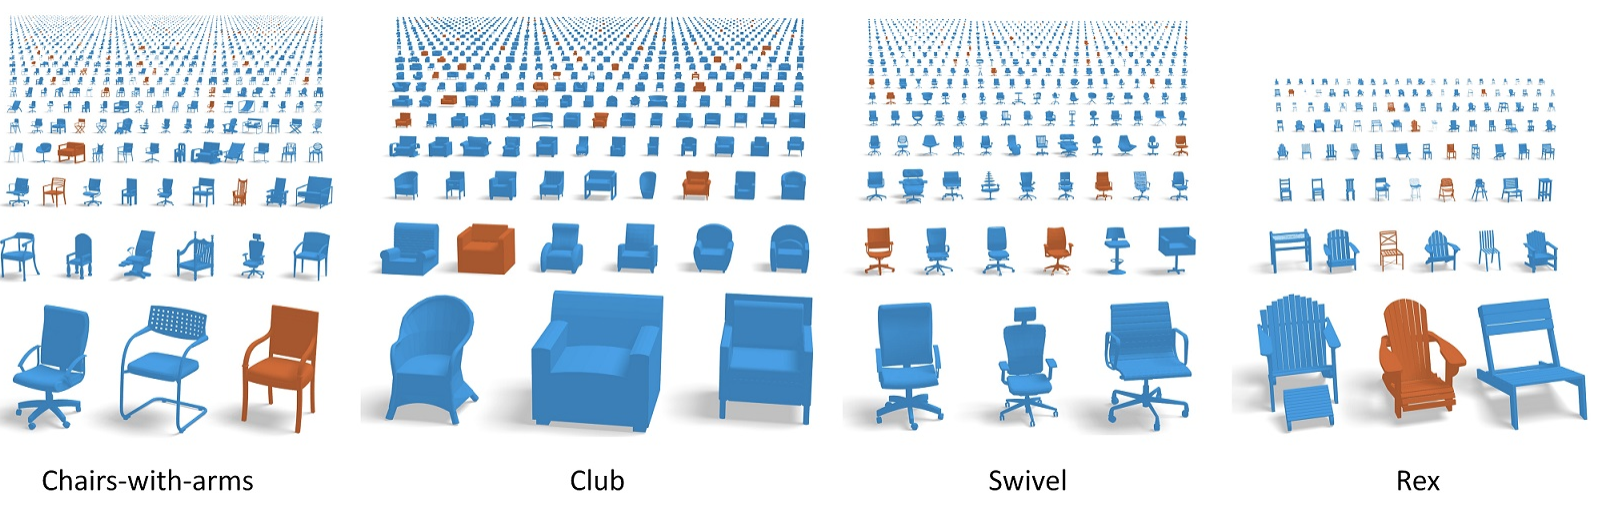
\includegraphics[width=1.0\columnwidth]{fig/search/huang_siga13_fine.png}
   %\vspace{-.6cm}
    \caption{
    Fine-grained classification of 3D models \cite{Huang:2013:FSL}, where text labels are propagated from brown to blue models. }
    \label{fig:fine-grained}
\end{figure}



\section{Shape classification}
\label{sec:classification}
% search / retrieval / classification
\rev{Data-driven techniques commonly make assumptions about the size and homogeneity of the input data set. In particular, existing analysis techniques often assume that all models belong to the same class of objects~\cite{Kim:2013:lpt} or scenes~\cite{Fisher:2011:CSR}, and cannot directly scale to entire repositories such as the Trimble 3D Warehouse~\cite{warehouse}. Similarly, techniques for data-driven reconstruction of indoor environments assume that the input data set only has furniture models~\cite{Nan:2012:SAC}, while modeling and synthesis interfaces restrict the input data to particular object or scene classes~\cite{Chaudhuri:2011:prabm,Kalogerakis:2012:PMC,Fisher:2012:CSR}.  Thus, as a first step these methods need to query a 3D model repository to retrieve a subset of relevant models.}

\rev{Most public shape repositories such as 3D Warehouse~\cite{warehouse} rely on the users to provide tags and names of the shapes with little additional quality control measures. As a result, the shapes are sparsely labeled with inconsistent and noisy tags.  This motivates developing automatic algorithms to infer text associated with models.  Existing work focuses on establishing class memberships for an entire shape (e.g. this shape is a chair), as well as inferring finer-scale attributes (e.g. this chair has a rocking leg).}


\rev{ \paragraph*{Classification} methods assign a class membership for unlabeled shapes. One approach is to retrieve for each unlabeled shape the most similar shape from a database of 3D models with known shape classes. There has been a large number of shape descriptors proposed in recent years that can be used in such a retrieval task, and one can refer to various surveys (e.g., \cite{Tangelder:2008:ASC}) for a thorough overview and comparisons. }
%
\rev{One can further improve classification results by leveraging machine learning techniques to learn classifiers that are based on global shape descriptors~\cite{Frome:2004:rord,Golovinskiy:2009:SBR3D}. Barutcuoglu et al.~\cite{Barutcuoglu:2006:hscu} demonstrate that Bayesian aggregation can be used to improve classification of shapes that are a part of a hierarchical ontology of objects. Geometry matching algorithms also facilitate distinguishing important features for classification~\cite{Funkhouser:2006:pm3d,Shilane:2007:drs}. Bronstein et al.\cite{Bronstein:2011:SGGW} leverage ``bag of features'' to learn powerful descriptor-space metrics for non-rigid shapes. These technique can be further improved by using sparse coding techniques~\cite{Litman:2014:SLBF} and perform well on benchmarks~\cite{Li:2012:SHREC,Li:2014:SHREC}.
%In recent shape retrieval challenges, techniques based on bag of features demonstrated the best performance~\cite{Li:2012:SHREC,Li:2014:SHREC} in comparison to other alternatives. 
\revnew{Motivated by the success of deep neural networks in image classification, Wu et al.~\cite{Wu:3SN:2015} represent a shape by a volumetric occupancy grid and train neural network to classify them. Su et al.~\cite{Su:MCN:2015} demonstrate that by rendering the shape from multiple viewpoints and analyzing the views as images enables leveraging the power of existing neural networks that were trained for image analysis. Su et al.~\cite{Su:2016aa} further combine both shape representations by sampling volumetric occupancy grids with anisotropic view-dependent kernels.}
%
See Table~\ref{tab:classification_performance} for a brief summary of some methods.}



% todo: figure for chaudhuri, for huang

\paragraph*{Tag attributes} often capture fine-scale attributes of shapes that belong to the same class.
These attributes can include presence or absence of particular parts, object style, or comparative adjectives.
%
Huang et al.~\cite{Huang:2013:FSL} developed a framework for propagating these attributes in a collection of partially annotated 3D models. For example, only brown models in Figure \ref{fig:fine-grained} were labeled, and blue models were annotated automatically. To achieve automatic labeling, they start by co-aligning all models to a canonical domain, and generate a voxel grid around the co-aligned models. For each voxel they compute local shape features, such as spin images, for each shape. Then, they learn a distance metric that best discriminates between different tags. All shapes are finally embedded in a weighted feature space where nearest neighbors are connected in a graph. A graph cut clustering is used to assign tags to unlabeled shapes.
%
\fix{Tag attributes can also be used to describe semantics, function, or style of parts in shapes. Data-driven consistent segmentation and labeling techniques can be applied to propagate part tags across shapes (see Section \ref{sec:segmentation}). An alternative approach is to partition shapes into multiple sets of parts, then extract descriptors to define part similarity. A characteristic example of such an approach was demonstrated in Shapira et al.~\cite{Shapira:2010:CPA}. Given the hierarchical segmentations of 3D shapes as input, part tagging was achieved by comparing local geometric features of parts as well as their context within the whole shape.}
%\fix{
%With hierarchical segmentation of 3D objects as input,
%Shapira et al.~\cite{Shapira:2010:CPA} propose contextual part analogies to achieve part tagging.
%To establish part-level correspondence among different 3D objects, a context enhanced part-in-whole matching where
%part similarity is measured based not only on local geometric signatures but also on their context within the whole shape.
%With such part analogies, textual tags of object parts can be carried from one model to others.
%}

\rev{ While the above method works well for discrete tags, they do not capture more continuous relations, such as animal A is more dangerous than animal B.  Chaudhuri et al.~\cite{Chaudhuri:2013:ACC} focus on estimating ranking based on comparative adjectives. They use crowdsourcing to gather pairwise comparisons of shape parts with respect to different adjectives, and use a Support Vector Machine ranking method to predict attribute strengths from shape features for novel shape parts (Figure \ref{fig:attribit}). }

\begin{figure}[tb]
\centering
    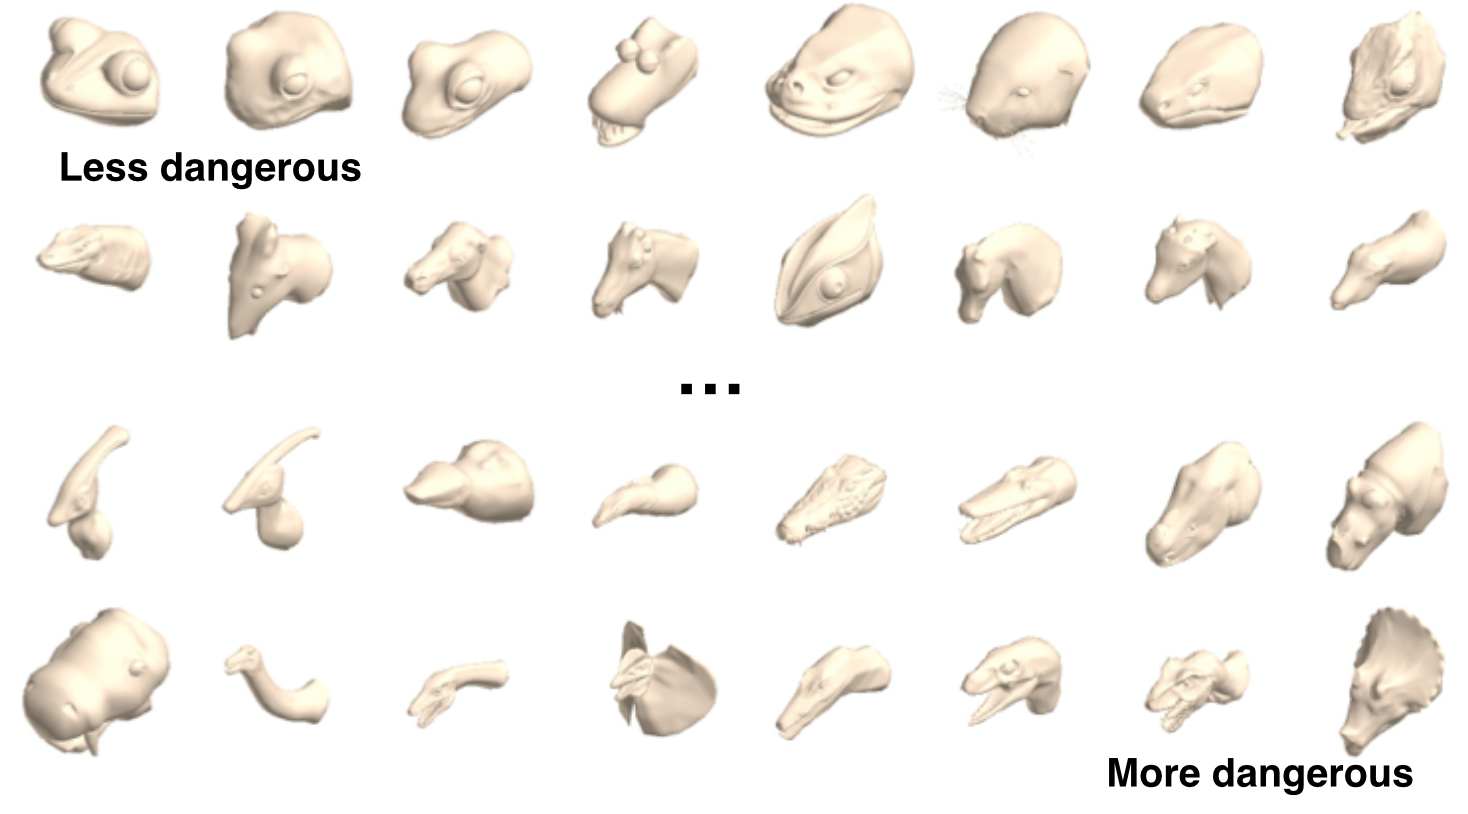
\includegraphics[width=1.0\columnwidth]{fig/search/chaudhuri_uist13_attr.png}
    %\vspace{-.6cm}
    \caption{
    Ranking of parts with respect to ``dangerous'' attribute (image from \cite{Chaudhuri:2013:ACC}) }
    \label{fig:attribit}
\end{figure}



\rev{ \paragraph*{Style similarity} methods have recently been proposed to classify shapes into style-related categories e.g., buildings can be classified into architectural styles, such as Gothic, Baroque, Byzantine and so on. In contrast to the previously discussed approaches that rely on generic visual similarity measures to compare shapes, these methods learn distance functions for style elements \cite{lun:style:2015} or common feature spaces \cite{liu:style:2015} to quantify the stylistic similarity of shapes. The methods can be used to compare the style similarity of shapes, even when these belong to different classes (e.g., chairs and lamps). To align the style similarity measures with the human perception of style, style comparisons of shapes are gathered through crowdsourcing.  The learned similarity measures can be used to retrieve stylistically similar shapes to populate a scene, or associate shapes with style-related tags. }

% limitations
%While the techniques described above are suitable for retrieving related models, most of the described method are not designed to understand intra-class variations. Usually a more involved structural analysis is necessary to understand higher-level semantic properties of shapes. Even for inferring tag attributes existing works relies on shape matching~\cite{Huang:2013:FSL} or shape segmentation~\cite{Chaudhuri:2013:ACC}. The following two sections will focus on inferring these higher-level structural properties in collections of shapes.

\rev{ While the techniques described above are suitable for retrieving and classifying shapes, a large number of applications require a more involved structural analysis to infer semantic and functional properties of shapes or their parts. The following two sections will discuss methods that perform structural analysis in collections of shapes based on segmentation and local matching.}



\begin{table*}[t!]
\small
  \centering
    \begin{tabular*}{\textwidth}{l|c|c|c|c|c@{}}
    \hline
    Segmentation                & Learning           & Type of          & PSB rand index (\# train. & L-PSB  accuracy (\# train.  & COSEG          \\
    method                      & type               & manual input     & shapes if applicable)     & shapes if applicable)       & accuracy       \\
    \hline
    \hline
    \cite{Kalogerakis:2010:LMS} & supervised         & labeled shapes   & 9.4\% (19) / 14.8\% (3)   & 95.3\% (19) / 89.2\% (3)    & unknown        \\
    \hline
    \cite{Benhabiles:2011:LBE}  & supervised         & segmented shapes & 8.8\% (19) / 9.7\% (6)    & not applicable              & not applicable \\
    \hline
    \cite{Huang:2011:JSS}       & unsupervised       & none             & 10.1\%                    & not applicable              & not applicable \\
    \hline
    \cite{Sidi:2011:CS}         & unsupervised       & none             & unknown                   & unknown                     & 87.7\%         \\
    \hline
    \cite{van-Kaick:2011:PKC}   & supervised         & labeled shapes   & unknown                   & \~88.7\% (12), see caption   & unknown        \\
    \hline
    \cite{Hu:2012:CSS}          & unsupervised       & none             & unknown                   & 88.5\%                      & 91.4\%         \\
    \hline
    \cite{Lv:2012:SMS}          & semi-supervised    & labeled shapes   & unknown                   & 92.3\% (3)                  & unknown        \\
    \hline
    \cite{Wang:2012:ACS}        & semi-supervised    & link constraints & unknown                   & unknown                     & `close to error-free' \\
    \hline
    \cite{Wang:2013:PAS}        & supervised         & labeled images   & unknown                   & \~88.0\% (19), see caption   & unknown               \\
    \hline
    \cite{Kim:2013:lpt}         & semi-/unsupervised & box templates    & unknown                   & unknown                     & 92.7\% (semi-superv.) \\
    \hline
    \cite{Huang:2014:FMN}       & unsupervised       & none             & unknown                   & unknown                     & 90.1\%                \\
    \hline
    \cite{Xu:2014:TSS}          & supervised         & labeled shapes   & 10.0\%                    & 86.0\%                      & unknown               \\
    \hline
    \cite{Zhige:2014:SSL}       & supervised         & labeled shapes   & 10.2\% (19)               & 94.2 (19) / 88.6 (5)        & unknown               \\
    \hline
    \end{tabular*}%
  \caption{\rev{Performance of data-driven methods for segmentation in the Princeton Segmentation Benchmark (PSB) and COSEG datasets.
		   Left to right: segmentation method, learning type depending on the nature of data required as input to the method, type of manual input if such required, segmentation performance expressed by the rand index metric \cite{Chen:2009:BMS}, labeling accuracy \cite{Kalogerakis:2010:LMS} based on the PSB and COSEG datasets. 	
  		   We report the rand index segmentation error metric averaged over all classes of the PSB benchmark.
  		   The labeling accuracy is averaged over the Labeled PSB (L-PSB) benchmark excluding the ``Bust'', ``Mech'', and ``Bearing'' classes. The reason is that there are no clear semantic correspondences between parts in these classes, or the ground-truth segmentations do not sufficiently capture semantic parts in their shapes.
  		   We report the labeling accuracy averaged over the categories of the COSEG dataset used in \cite{Sidi:2011:CS}. The COSEG classes ``iron'', ``large chairs'', ``large vases'', ``tele-aliens'' were added later and are excluded here since most papers frequently do not report performance in those.
  		   We note that van Kaick et al.~\cite{van-Kaick:2011:PKC} reported the labeling accuracy in ten of the L-PSB classes, while Wang et al.~\cite{Wang:2013:PAS}  reported the labeling accuracy in seven of the L-PSB classes.
  		   The method by Kim et al.~\cite{Kim:2013:lpt} can run in either semi-supervised or unsupervised mode. In unsupervised mode, the corresponding labeling accuracy is 89.9\% in the COSEG dataset on average.
  		   }}
  \label{tab:segmentation_performance}%
\end{table*}


\section{Shape segmentation}
\label{sec:segmentation}

The goal of data-driven shape segmentation is to partition the shapes of an input collection into parts, and also estimate part correspondences across these shapes. We organize the literature on shape segmentation into the following three categories: supervised segmentation, unsupervised segmentation, and semi-supervised segmentation following the main classification discussed in Section \ref{sec:overview}. \rev{Table \ref{tab:segmentation_performance} summarizes representative techniques and reports their segmentation and part labeling performance based on established benchmarks. Table \ref{tab:segmentation_running_times} reports characteristic running times for the same techniques.}

%For example, a data-driven segmentation algorithm can segment the shapes of an input collection of chairs into parts, such as legs, back, and seat.

%There is no unique way to segment a shape:
%the user can provide a set of exemplar shape segmentations, desired part correspondences, or parameters to control the type and level of detail for segmentation. Alternatively, shapes can be consistently segmented at various levels of detail, and the segments can be organized hierarchically.

\begin{figure}[t]
\centering
    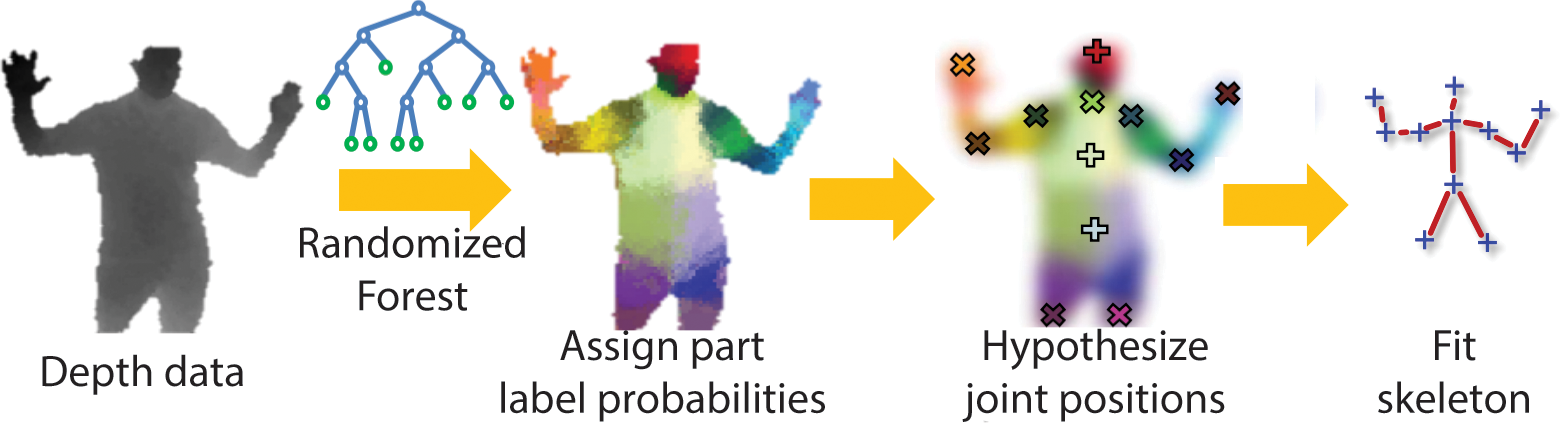
\includegraphics[width=1.0\columnwidth]{fig/img/kinect}
    %\vspace{-0.4cm}
    \caption{
    A random forest classifier applied on depth data representing a human body shape (image from \protect\cite{Fossati:2013:CDC}) }
    \label{fig:kinect}
\end{figure}



\subsection{Supervised shape segmentation}

\paragraph*{Classification techniques.} Supervised shape segmentation is frequently formulated as a classification problem. Given a training set of shapes containing points, faces or patches that are labeled according to a part category (see Figure \ref{fig:overview_seg}), the goal of a classifier is to identify which part category other points, faces, or patches from different shapes belong to. Supervised shape segmentation is executed in two steps: during the first step, the parameters of the classifier are learned from the training data. During the second step, the classifier is applied on new shapes. A simple linear classifier has the form:
\begin{equation}
c = f ( \sum\limits_j \theta_j \cdot x_j )
\end{equation}
where $x_j$ is a geometric feature of a point (face, or patch), such as the ones discussed in Section \ref{sec:overview}. The parameters $\theta_j$ serve as weights for each geometric feature. The function $f$ is non-linear and maps to a discrete value (label), which is a part category, or to probabilities per category. In general, choosing a good set of geometric features that help predicting part labels, and employing classifiers that can discriminate the input data points correctly are important design choices. There is no rule of thumb on which is the best classifier for a problem. This depends on the underlying distribution and characteristics of the input geometric features, their dimensionality, amount of labeled data, existence of noise in the labeled data or shapes, training and test time constraints - for a related discussion on how to choose a classifier for a problem, we refer the reader to \cite{Manning:2008:IIR}. Due to the large dimensionality and complexity of geometric feature spaces, non-linear classifiers are more commonly used. For example, to segment human bodies into parts and recognize poses, the Microsoft's Kinect uses a random forest classifier trained on synthetic depth images of humans of many shapes and sizes in highly varied poses sampled from a large motion capture database \cite{Shotton:2011:RLH} (Figure \ref{fig:kinect}).


\paragraph*{Structured models.} For computer graphics applications, it is important to segment shapes with accurate and smooth boundaries. For example, to help the user create a new shape by re-combining parts from other shapes \cite{Funkhouser:2004:MBE}, irregular and noisy segmentation boundaries can cause problems in the part attachment. From this aspect, using a classifier per point/face independently is usually not enough. Thus, it is more common to formulate the shape segmentation problem as an energy minimization problem that involves a unary term assessing the consistency of each point/face with each part label, as well as a pairwise term assessing the consistency of neighboring points/faces with pairs of labels. For example, pairs of points that have low curvature (i.e., are on flat surface) are more likely to have the same part label. This energy minimization formulation has been used in several single-shape and data-driven segmentations (unsupervised or supervised) \cite{Katz:2003:HMD,Anguelov:2005:DLM,Shapira:2010:CPA,Kalogerakis:2010:LMS}. In the case of supervised segmentation \cite{Kalogerakis:2010:LMS}, the energy can be written as:
\begin{equation}
E(\bc; \theta) = \sum_i E_{unary}(c_i; \bx_i, \theta_1) + \sum_{i,j} E_{pairwise}(c_i, c_j; \by_{ij}, \theta_2)
\label{eqn:CRFEnergy}
\end{equation}
where $\bc=\{c_i\}$ is a vector of random variables representing the part label per point (or face) $i$, $\bx_i$ is its geometric feature vector, $i,j$ are indices to points (or faces) that are considered neighbors, $\by_{ij}$ is a geometric feature vector representing dihedral angle, angle between normals, or other features, and $\theta=\{\theta_1,\theta_2\}$  are the energy parameters.  The important difference of supervised data-driven methods with previous single-shape segmentation methods is that the parameters $\theta$ are automatically learned from the training shapes to capture complex feature space patterns per part \cite{Anguelov:2005:DLM,Kalogerakis:2010:LMS}. We also note that the above energy of Equation \ref{eqn:CRFEnergy}, when written in an exponentiated form and normalized, can be treated as a probabilistic graphical model \cite{Koller:2009:PGM}, called Conditional Random Field \cite{Lafferty:2001:CRF} that represents the joint probability distribution over part labels conditioned on the input features:
\begin{equation}
P(\bc | \bx, \by, \theta)= \exp(-E(\bc;\theta))/ Z(\bx,\by,\theta)
\label{eqn:CRFConditional}
\end{equation}
where $Z(\bx,\by,\theta)$ is a normalization factor, also known as partition function. \rev{Minimizing the energy of Equation \ref{eqn:CRFEnergy}, or correspondingly finding the assignment $\bc$ that maximizes the above probability distribution is known as a Maximum A Posteriori inference problem that can be solved in various manners, such as graph cuts, belief propagation, variational or linear programming relaxation techniques \cite{Koller:2009:PGM}.}


The parameters $\theta$ can be jointly learned through maximum likelihood (ML) or maximum a posteriori (MAP) estimates \cite{Koller:2009:PGM}. However, due to high computational complexity of ML or MAP learning and the non-linearity of classifiers used in shape segmentation, it is common to train the parameters $\theta_1$ and $\theta_2$ of the model separately i.e., train the classifiers of the unary and pairwise term separately \cite{Sutton:2005:PTU}. The exact form of the unary and pairwise terms vary across supervised shape segmentation methods: the unary term can have the form of a log-linear model \cite{Anguelov:2005:DLM}, cascade of JointBoost classifiers \cite{Kalogerakis:2010:LMS}, Gentleboost \cite{van-Kaick:2011:PKC}, or feedforward neural networks \cite{Zhige:2014:SSL}. The pairwise term can have the form of a learned log-linear model \cite{Anguelov:2005:DLM}, label-dependent GentleBoost classifier \cite{Kalogerakis:2010:LMS}, or a smoothness term based on dihedral angles and edge length tuned by experimentation \cite{Shapira:2010:CPA,van-Kaick:2011:PKC,Zhige:2014:SSL}. Again the form of the unary and pairwise terms depend on the amount of training data, dimensionality and underlying distribution of geometric features used, and computational cost.


\begin{table*}[t!]
\small
  \centering
    \begin{tabular}{l|c|c|c}
    \hline
    Segmentation                & Reported                     &  Dataset size for       & Reported \\
    method                      & running times                &  reported running times & processor \\
    \hline
    \hline
    \cite{Kalogerakis:2010:LMS} & 8h train. / 5 min test.      &  6 train. shapes / 1 test shape     & Intel Xeon E5355 2.66GHz \\
    \hline
    \cite{Benhabiles:2011:LBE}  & 10 min train. / 1 min test.  &  unknown for train. / 1 test shape  & Intel Core 2 Duo 2.99GHz \\
    \hline
    \cite{Huang:2011:JSS}       & 32h                          &  380 shapes                         & unknown, 2.4 GHz \\
    \hline
    \cite{Sidi:2011:CS}         & 10 min                       &  30 shapes                          & AMD Opteron 2.4GHz \\
    \hline
    \cite{van-Kaick:2011:PKC}   & 10h train. / few min test.   &  20-30 train. shapes / 1 test shape & AMD Opteron 1GHz  \\
    \hline
    \cite{Hu:2012:CSS}          & 8 min (excl. feat. extr.)    &  20 shapes                          & Intel dual-core 2.93GHz  \\
    \hline
    \cite{Lv:2012:SMS}          & 7h train. / few min test.    &  20 shapes                          & Intel I7 2600 3.4GHz \\
    \hline
    \cite{Wang:2012:ACS}        & 7 min user interaction       &  28 shapes                          & unknown \\
    \hline
    \cite{Wang:2013:PAS}        & 1.5 min (no train. step)     &  1 test shape                       & unknown \\
    \hline
    \cite{Kim:2013:lpt}         & 11h                          &  7442 shapes                        & unknown \\
    \hline
    \cite{Huang:2014:FMN}       & 33h                          &  8401 shapes                        & unknown, 3.2GHZ \\
    \hline
    \cite{Xu:2014:TSS}          & 30 sec (no train. step)      &  1 test shape                       & Intel I5 CPU \\
    \hline
    \cite{Zhige:2014:SSL}       & 15 sec train. (excl. feat. extr.) &  6 train. shapes                & Intel Quad-Core 3.2 GHz \\
    \hline
    \end{tabular}%
  \caption{\rev{Running times reported for the data-driven segmentation methods of Table \ref{tab:segmentation_performance}. We note that running times are reported in different dataset sizes and processors in the referenced papers, while it is frequently not specified whether the execution uses one or multiple threads or whether the running times include all the algorithm steps, such as super-face or feature extraction.
           Exact processor information is also frequently not provided. Thus, the reported running times of this table are only indicative and should not serve as a basis for a fair comparison.}}
  \label{tab:segmentation_running_times}%
\end{table*}



\paragraph*{Joint labeling.} Instead of applying the learned probabilistic model to a single shape, an alternative approach is to find correspondences between faces of pairs of shapes, and incorporate a third ``inter-shape'' term in the energy of Equation \ref{eqn:CRFEnergy} \cite{van-Kaick:2011:PKC}. The ``inter-shape'' term favors pairs of corresponding faces on different shapes to have the same label. As a result, the energy can be minimized jointly over a set of shapes to take into account any additional correspondences.



\paragraph*{Boundary learning.} Instead of applying a classifier per mesh point, face or patch to predict a part label, a different approach is to predict the probability that a polygon mesh edge is a segmentation boundary \cite{Benhabiles:2011:LBE}. The problem can be formulated as a binary classifier (e.g., Adaboost) that is trained from human segmentation boundaries. The input to the classifier are geometric features of edges, such as dihedral angles, curvature, and shape diameter. The output is a probability for an edge to be a segmentation boundary. Since the predicted probabilities over the mesh do not correspond to closed smooth boundaries, a thinning and an active contour model \cite{Kass:1988:SAC} are used in post-processing to produce the final segmentations.
%The output is not a labeled segmentation as in previous techniques, but a set of candidate segmentation boundaries. The method has currently the best performance in segmentation according to the Rand Index criterion in the PSB benchmark \cite{Chen:2009:BMS}.

\paragraph*{Transductive segmentation.} Another way to formulate the shape segmentation problem is to group patches on a mesh such that the segment similarity is maximized between the resulting segments and the provided segments in the training database. The segment similarity can be measured as the reconstruction cost of the resulting segment from the training ones. The grouping of patches can be solved as an integer programming problem \cite{Xu:2014:TSS}.

\paragraph*{Shape segmentation from labeled images.} \rev{Instead of using labeled training shapes for supervised shape segmentation, an alternative source of training data can come in the form of segmented and labeled images, as demonstrated by Wang et al. \cite{Wang:2013:PAS}. Given an input 3D shape, this method first renders 2D binary images of it from different viewpoints. Each binary image is used to retrieve multiple segmented and labeled training images from an input database based on a bi-class Hausdorff distance measure. Each retrieved image is used to perform label transfer to the 2D shape projections. All labeled projections are then back-projected onto the input 3D model to compute a labeling probability map. The energy function for segmentation is formulated by using this probability map in the unary term expressed per face or point, while dihedral angles and Euclidean distances are used in the pairwise term.}


\subsection{Semi-supervised shape segmentation}

\paragraph*{Entropy regularization.} The parameters $\theta$ of \rev{Equation \ref{eqn:CRFEnergy}} can be learned not only from the training labeled shapes, but also from the unlabeled shapes \cite{Lv:2012:SMS}. The idea is that learning should maximize the likelihood function of the parameters over the labeled shapes, and also minimize the entropy (uncertainty) of the classifier over the unlabeled shapes (or correspondingly maximize the negative entropy). The idea is that minimizing the entropy over unlabeled shapes encourages the algorithm to find putative labelings for the unlabeled data \cite{Jiao:2006:SCR}. However, it is generally hard to strike a balance between the likelihood and entropy terms.

\paragraph*{Metric embedding and active learning.} A more general formulation for semi-supervised segmentation was presented in \cite{Wang:2012:ACS}.
%(Figure \ref{fig:active_coanalysis}).
Starting from a set of shapes that are co-segmented in an unsupervised manner \cite{Sidi:2011:CS}, the user interactively adds two types of constraints: ``must-link'' constraints, which specify that two patches (super-faces) should belong to the same cluster, and ``cannot-link'' constraints which specify that two patches  must be in different clusters. These constraints are used to perform constrained clustering in an embedded feature space of super-faces coming from all the shapes of the input dataset. The key idea is to transform the original feature space, such that super-faces with ``must-link'' constraints come closer together to form a cluster in the embedded feature space, while super-faces with ``cannot-link'' constraints move away from each other. To minimize the effort required from the user, the method suggests to the user pairs of points in feature space that when constrained are likely to improve the co-segmentation.  The suggestions involve points that are far from their cluster centers, and have a low confidence of belonging to their clusters.

\paragraph*{Template fitting.} \rev{A different form of partial supervision can come in the form of part-based templates. Kim et al.'s method \cite{Kim:2013:lpt} allows users to specify or refine a few templates made out of boxes representing expected parts in an input database. The boxes iteratively fit to the shapes of a collection through simultaneous alignment, surface segmentation and point-to-point correspondences estimated between each template and each input shape. Alternatively, the templates can be inferred automatically from the shapes of the input collection without human supervision based on single shape segmentation heuristics. Optionally, the user can refine and improve these estimated templates. From this aspect, Kim et al.'s method can run in either a semi-supervised or unsupervised method. It was also the first method to handle segmentation and correspondences in collections with size on the order of thousands of shapes.}


\subsection{Unsupervised segmentation}

Unsupervised data-driven shape segmentation techniques fall into two categories: clustering based techniques and matching based techniques. In the following, we highlight the key idea of each type of approach.
% and review representative works.

\para{Clustering} based techniques are adapted from supervised techniques. They compute feature descriptors on points or faces. Clustering is performed over all points/faces over all shapes. Each resulting cluster indicates a consistent segment across the input shapes. The promise of the clustering based approach is that when the number of shapes becomes large, the sampling density in the clustering space becomes dense enough, so that certain statistical assumptions are satisfied, e.g., diffusion distances between points from different clusters is significantly larger than those between points within each cluster. \rev{When these assumptions are satisfied, clustering based approaches may produce results that are comparable to supervised techniques (c.f.~\cite{Hu:2012:CSS}) . In~\cite{Sidi:2011:CS}, the authors utilize spectral clustering to perform clustering. In~\cite{Hu:2012:CSS}, the authors employ subspace clustering, a more advanced clustering method, to obtain improved results.}

Clustering methods can also be applied to shape parts. In~\cite{Xu:2010:SCS}, the authors perform co-analysis over a set of shapes via factoring out the part scale variation by grouping the shapes into different styles, where style is defined by the anisotropic part scales of the shapes. In~\cite{van-Kaick:2013:CHA}, the authors introduce unsupervised co-hierarchical analysis of a set of shapes. They propose a novel cluster-and-select scheme for selecting representative part hierarchies for all shapes and grouping the shapes according to the hierarchies. The method can be used to compute consistent hierarchical segmentations for the input set.

\begin{figure}[t!]
\centering
    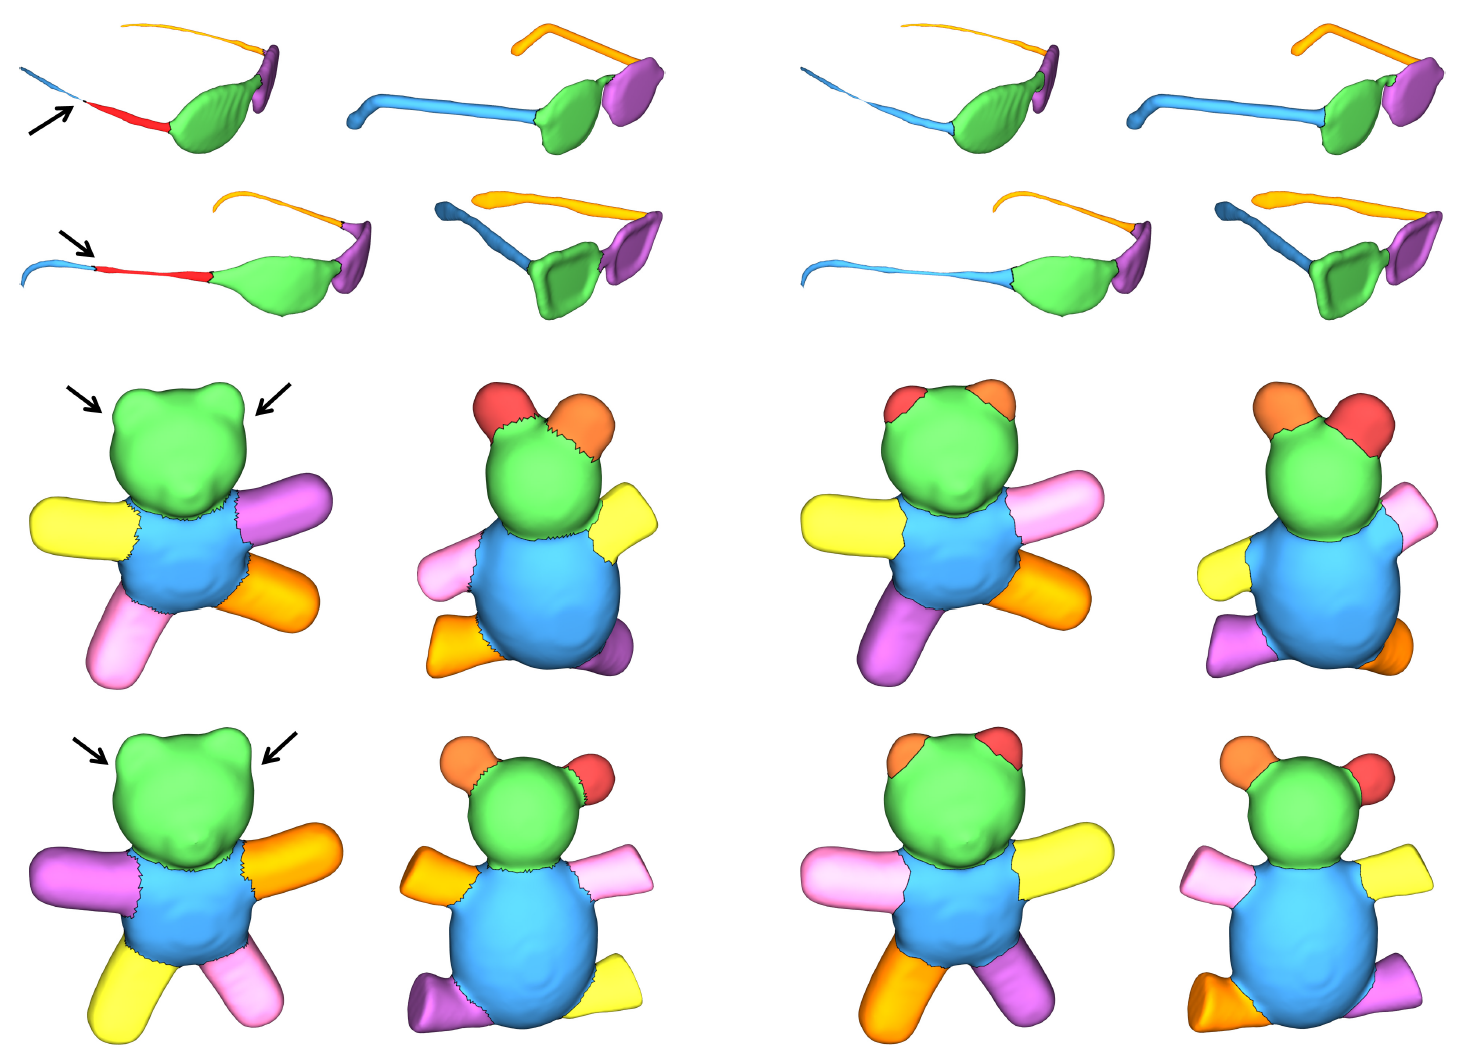
\includegraphics[width=1.0\columnwidth]{fig/img/huang_siga11_jss.png}
    %\vspace{-0.5cm}
    \caption{Comparison of single-shape segmentation (left) and joint shape segmentation (right) on models from the PSB benchmark~\cite{Chen:2009:BMS}. Each segmentation on the left was produced by the top-performing algorithm in the benchmark for that shape. The segmentations on the right were produced
by~\cite{Huang:2011:JSS}, which jointly optimized segmentations and correspondences across the entire dataset.}
    \label{fig:huang_siga11_jss}
\end{figure}



\para{Matching} based methods~\cite{Golovinskiy:2009:CS,Huang:2011:JSS,Wang:2013:FMap,Huang:2014:FMN} build maps across shapes and utilize these maps to achieve consistency of segmentations. As shown in Figure~\ref{fig:huang_siga11_jss}, this strategy allows us to identify meaningful parts despite the lack of strong geometric cues on a particular shape. Likewise, the approach is able to identify coherent single parts even when the geometry of the individual shape suggests the presence of multiple segments. A challenge here is to find a suitable shape representation so that maps across diverse shapes are well-defined. In~\cite{Huang:2011:JSS}, Huang et al. introduce an optimization strategy that jointly optimizes shape segmentations and maps between optimized segmentations. Since the maps are defined at the part-level, this technique is suitable for heterogeneous shape collections. Experimentally, it generates comparable results with supervised method~\cite{Kalogerakis:2010:LMS} on the Princeton segmentation benchmark.  Recently, Huang et al.\cite{Huang:2014:FMN} formulated the same idea under the framework of functional maps~\cite{Ovsjanikov:2012:FMF} and gain improved segmentation quality and computational efficiency.


\section{Joint shape matching}
\label{sec:matching}

Another fundamental problem in shape analysis is shape matching, which finds relations or maps between shapes. These maps allow us to transfer information across shapes and aggregate information from a collection of shapes for a better understanding of individual shapes (e.g., detecting shared structures such as skeletons or shape parts). \rev{They also provide a powerful platform for comparing shapes (i.e., with respect to different measures and at different places). As we can see from other sections, shape maps are widely applied in shape classification and shape exploration as well.}

So far, most existing research in shape matching has focused on matching pairs of shapes in isolation. We refer to~\cite{van-Kaick:2010:SSC} for a survey and to~\cite{Leordeanu:2005:SM,Lipman:2009:MVC,van-Kaick:2010:SSC,Ovsjanikov:2010:OPM,Kim:2011:BIM,Ovsjanikov:2012:FMF} for recent advances. Although significant progress has been made,
state-of-the-art techniques are limited to shapes that are similar to each other. \rev{On the other hand, these techniques tend to be insufficient among shape collections that possess large geometric and topological variations.}

The availability of large shape collections offers opportunities to address this issue. Intuitively, when matching two dissimilar shapes, we may utilize intermediate shapes to transfer maps. In other words, we can build maps between similar shapes, and use the composite maps to obtain maps between less similar shapes. As we will see shortly, this intuition can be generalized to enforcing a cycle-consistency constraint; namely composite maps along cycles should be the identity map and the composite map between any two shapes is path-independent.
%
In this section, we discuss joint shape matching techniques that take a shape collection and noisy maps as input, and output improved maps across the shape collection.
%In a broader picture, the problem of joint matching is related to a wide range of topics, including fusing partially overlapped range scans~\cite{Huber:2002:Thesis}, re-assembling fractured objects~\cite{Huang:2006:RFO}, solving jigsaw puzzles~\cite{Goldberg:2004:GAA,Cho:2010:JPS}, and DNA/RNA sequencing and modeling~\cite{Marande:2007:DNA}. In the following, we focus on the contributions most related to 3D shapes.

\subsection{Model graph and cycle-consistency}

To formulate the joint matching problem, we consider a model graph $\set{G} = (\set{S}, \mathcal{E})$ (c.f.~\cite{Huber:2002:Thesis}). The vertex set $\set{S} = \{S_1, \cdots, S_{n})\}$ consists of the input shapes. The edge set $\set{E}$ characterizes the pairs of shapes that are selected for performing pair-wise matching. For small-scale datasets, we typically match all pairs of shapes. For large-scale datasets, the edge set usually connects shapes that are similar according to a pre-defined shape descriptor~\cite{Kim:2012:FC,Huang:2013:FSL}, thus generating a sparse shape graph.

The key component of a joint matching algorithm is to utilize the so-called cycle-consistency constraint.  In particular, if all the maps in $\mathcal{G}$ are correct, then composite maps along any loops should be the identity map. This is true for maps that are represented as transformations (e.g., rotations and rigid/affine transformations), or full point-wise maps that can be described as permutation matrices). We can easily modify the constraint to handle partial maps; namely, each point, when transformed along a loop, either disappears or goes back to the original point (See \cite{Huang:2014:FMN} for details).

The cycle-consistency constraint is useful because the initial maps, which are computed between pairs of shapes in isolation, are not expected to satisfy the cycle consistency constraint. \rev{On the other hand, although we do not know which maps or correspondences are incorrect, we can detect inconsistent cycles.} These inconsistent cycles provide useful information for us to detect incorrect correspondences or maps, i.e., an inconsistent cycle indicates that at least one of the participating maps or correspondences is incorrect. To incorporate this observation into algorithms, one has to formulate the cycle-consistency constraint properly. Existing works in data-driven shape matching fall into two categories: combinatorial techniques and matrix recovery based techniques.  The reminder of this section provides the details.

\begin{figure}[t]
\centering
    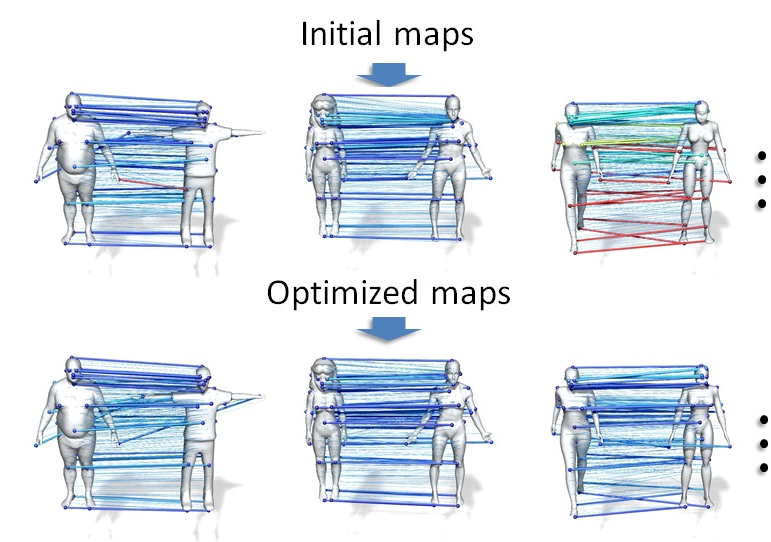
\includegraphics[width=1.0\columnwidth]{fig/img/huang_sig14_jsm.png}
    %\vspace{-0.4cm}
    \caption{Joint shape matching takes as input maps computed between pairs of shapes in isolation and utilizes the cycle-consistency constraint to improve shape maps. This figure shows the result of Huang et al.~\protect\cite{Huang:2014:FMN}, which performs joint shape matching under the functional map setting.}
    \label{fig:huang_sig14_jsm}
\end{figure}



\subsection{Combinatorial techniques}

\para{Spanning tree optimization.} Earlier works in joint matching aim at finding a spanning tree in the model graph. In~\cite{Goldberg:2004:GAA,Huang:2006:RFO}, the authors propose to use the maximum spanning tree (MST) of the model graph. However, this strategy can easily fail since a single incorrect edge in the MST may break the entire matching result. In the seminal work~\cite{Huber:2002:Thesis}, Huber showed that finding the best spanning tree maximizing the number of consistent edges is NP-hard. Although finding the best spanning tree is not tractable, Huber introduced several local operations for improving the score of spanning trees. \rev{However, these approaches are generally limited to small-scale problems so that the search space can be sufficiently explored.}

\para{Inconsistent cycle detection.} Another line of approaches~\cite{Zach:2010:DVR,Roberts:2011:SFM,Nguyen:2011:CSM} applies global optimization to select cycle-consistent maps. These approaches are typically formulated as solving constrained optimization problems, where objective functions encode the scores of selected maps, and constraints enforce the consistency of selected maps along cycles. The major advantage of these approaches is that the correct maps are determined globally. However, as the cycle consistency constraint needs to apportion blame along many edges on a cycle, the success of these approaches relies on the assumption that correct maps are dominant in the model graph so that the small number of bad maps can be identified through their participation in many bad cycles.

\para{MRF formulation.} Joint matching may also be formulated as solving a second order Markov Random Field (or MRF)~
\cite{Cho:2010:JPS,Cho:2010:TPT,Crandall:2011:DOL,Huang:2012:OAE}. The basic idea is to sample the transformation/deformation space of each shape to obtain a candidate set of transformation/deformation samples per shape. Joint matching is then formulated as optimizing the best sample for each shape. The objective function considers initial maps. Specifically, each pair of samples from two different shapes would generate a candidate map between them. The objective function then formulates second-order potentials, where each term characterize the alignment score between these candidate maps and the initial maps~\cite{Huang:2013:FSL,Huang:2012:OAE}.

The key challenge in the MRF formulation is generating the candidate samples for each shape. The most popular strategy is to perform uniform sampling~\cite{Crandall:2011:DOL,Huang:2013:FSL}, which works well when the transformation space is low-dimensional. To apply the MRF formulation on high-dimensional problems, Huang et al.~\cite{Huang:2012:OAE} introduce a diffusion-and-sharpening strategy. The idea is to diffuse the maps among the model graph to obtain rich samples of candidate transformations or correspondences and then perform clustering to reduce the number of candidate samples.


\subsection{Matrix based techniques}



A recent trend in map computation is to formulate joint map computation as inferring matrices~\cite{Singer:2011:VDM,Huang:2012:OAE,Kim:2012:FC,Huang:2013:SDP,journals/corr/abs-1211-2441,Chen:2014:SDP,Huang:2014:FMN}. The basic idea is to consider a big map collection matrix
$$
\vec{X} = \left [
\begin{array}{cccc}
\vec{X}_{11} & \vec{X}_{12} & \cdots & \vec{X}_{1n} \\
\vec{X}_{21} & \vec{X}_{22} & \cdots & \vec{X}_{2n} \\
\vdots & \ddots & \cdots & \vdots \\
\vec{X}_{21} & \cdots & \cdots & \vec{X}_{nn}
\end{array}
\right],
$$
where each block $\vec{X}_{ij}$ encodes the map from shape $S_i$ to shape $S_j$. In this matrix representation, the cycle-consistency constraint can be equivalently described by simple properties of $\vec{X}$, i.e., depending on the types of maps, $\vec{X}$ is either positive semidefinite or low-rank (c.f.~\cite{Huang:2013:SDP,Huang:2014:FMN}). In addition, we may view the initial pair-wise maps as noisy measurements of the entries of $\vec{X}$. Based on this perspective, we can formulate joint matching as matrix recovery from noisy measurements of its entries.

\para{Spectral techniques.} The initial attempts in matrix recovery are spectral techniques and their variants~\cite{Singer:2011:VDM,Kim:2012:FC,Wang:2013:FMap}. The basic idea is to consider the map collection $\vec{X}^{\textup{input}}$ that encodes initial maps in its blocks. Then, the recovered matrix is given by $\vec{X} = \vec{U}\Sigma \vec{V}^{T}$, where $\vec{U}, \Sigma, \vec{V}$ represent the singular value decomposition (or SVD) of $\vec{X}^{\textup{input}}$. Various methods have added heuristics on top of this basic procedure. For example, Kim et al.~\cite{Kim:2012:FC} use the optimized maps to recompute initial maps.

This SVD strategy can be viewed as matrix recovery because $\vec{X}$ is equivalent to the optimal low-rank approximation of $\vec{X}^{\textup{input}}$ (with given rank) under the matrix Frobenius norm. However, as the input maps may contain outliers, employing the Frobenius norm for matrix recovery is sub-optimal. Moreover, it is hard to analyze these techniques, even in the very basic setting where maps are given by permutation matrices~\cite{conf/nips/PachauriKS13}.


\begin{figure}[t!]
\centering
    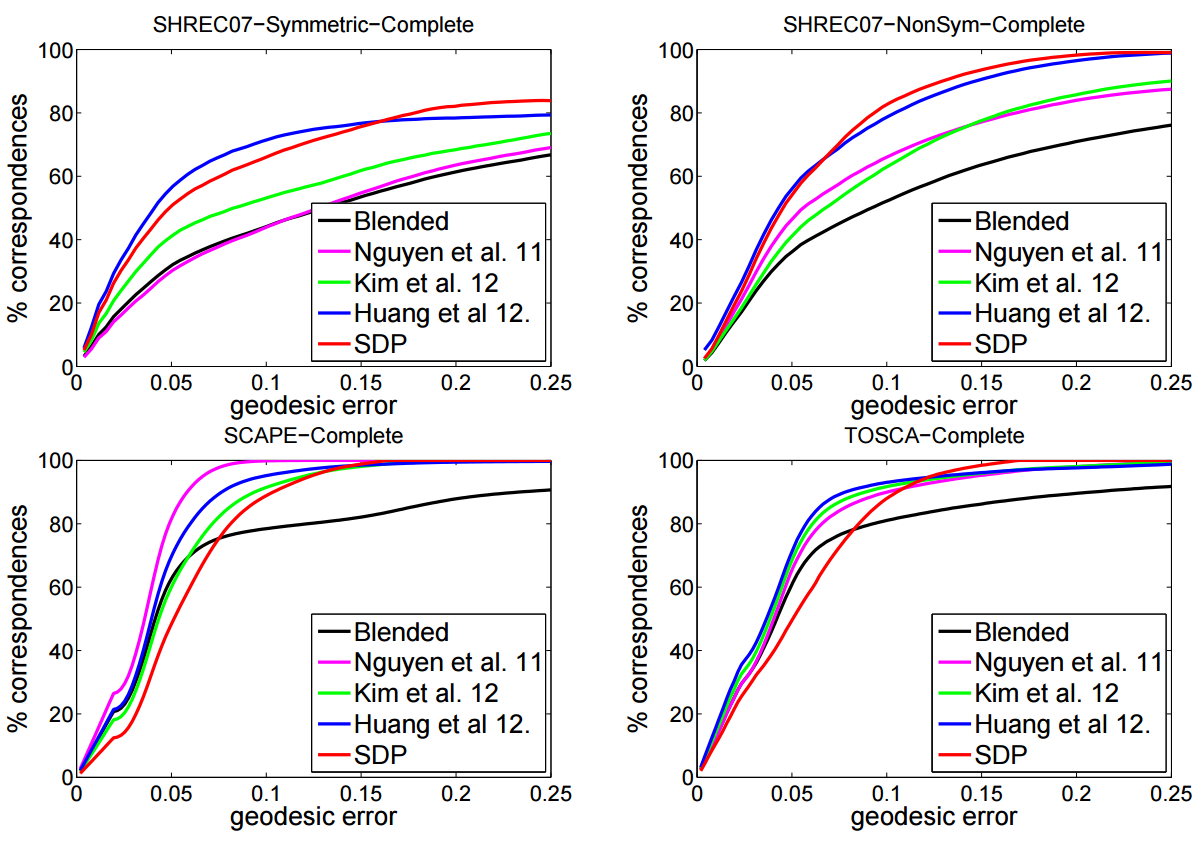
\includegraphics[width=1.0\columnwidth]{fig/img/map_evaluation.png}
    \vspace{-.5cm}
    \caption{\rev{Comparison among various data-driven shape matching methods: optimized composite maps~\protect\cite{Nguyen:2011:CSM}, fuzzy correspondences~\protect\cite{Kim:2012:FC},
hub-and-spoke network~\protect\cite{Huang:2012:OAE} and semidefinite programming relaxation~\protect\cite{Huang:2013:SDP}. The input maps are given by blended
intrinsic maps~\protect\cite{Kim:2011:BIM}.}}
    \label{fig:map_evaluation}
\end{figure}

\para{Point-based maps.} In a series of works, Huang and coworkers~\cite{Huang:2013:SDP,Chen:2014:SDP,cg-ssrmrf-14} consider the case of point-based maps and develop joint matching algorithms that admit theoretical guarantees. The work of~\cite{Huang:2013:SDP} considers the basic setting of permutation matrix maps and proves the equivalence between cycle-consistent maps and the low-rank or positive semi-definiteness of the map collection matrix. This leads to a semidefinite programming formulation for joint matching. In particular, the L1 norm is used to measure the distance between the recovered maps and the initial maps. The authors provide exact recovery conditions, which state that the ground-truth maps can be recovered if the percentage of incorrect correspondences in the input maps is below a constant. \rev{In a followup work, Chen et al.~\cite{Chen:2014:SDP} extends this to partial maps and provide a better analysis in the case where incorrect correspondences in the input maps are random.} The computational issue is addressed in~\cite{cg-ssrmrf-14}, which employs the alternating direction of multiplier methods for optimization. Figure~\ref{fig:map_evaluation} compares the SDP formulation of~\cite{Huang:2013:SDP} with several other data-driven shape matching methods. Note that all data-driven shape matching methods improve upon pair-wise matching, yet the SDP formulation leads to the largest improvement.

\para{Rotations and functional maps.} Maps that are represented by general matrices (e.g., rotations or functional maps) can also be handled in a similar fashion. In~\cite{journals/corr/abs-1211-2441}, Wang and Singer consider the case of rotations between objects. Their formulation is similar to~\cite{Huang:2013:SDP} but utilize an L1 Frobenius norm for measuring the distance between initial rotations and recovered rotations. Recently, Huang et al.~\cite{Huang:2014:FMN} extend this idea to functional maps. The major difference between functional maps and point-based maps or rotations is that the map collection matrix is no-longer symmetric. Thus, their method is formulated to recover low-rank matrices.


\subsection{Discussion and future directions}

The key to joint shape matching is to have a proper formulation of the cycle-consistency constraint. We have witnessed the evolution of this constraint from earlier works on combinatorial search and inconsistent cycle detection to more recent works which use spectral techniques, MRF based methods and matrix recovery techniques. In particular, matrix recovery techniques admit theoretical guarantees, providing a fundamental understanding of why joint shape matching can improve upon isolated pair-wise matching.

One future direction is to integrate pair-wise matching and joint matching into one optimization problem. Since the major role of joint matching is to remove the noise presented in pair-wise matching, it makes sense to perform them together. Such unified approaches have the potential to further improve upon decomposed approaches (i.e., from pair-wise to joint). The technical challenge is to find map representations so that pair-wise matching and map consistency can be formulated in the same framework.

%As we will discuss later, one of applications of map computation is in organizing big geometric data. Thus, it is important to develop data-driven matching techniques that are scalable to big geometric data. None of existing data-driven shape matching techniques can handle shape collections with more than thousands of shapes. In a recent paper, Huang et al.~\cite{Huang:2014:FMN} introduce a multi-layer map computation framework so that map computation may be distributed. The method essentially divide the input data into clusters and perform joint map computation among each cluster independently. The next layer builds maps between clusters. Maps between shapes are composed from maps with clusters and cluster-maps.  Still, there are plenty of open questions left including how to build the hierarchical map structure and what is the fundamental difference between a multi-layer structure and a single-layer structure (e.g., the techniques described above).


\section{Shape reconstruction}
\label{sec:recon}

Reconstructing geometric shapes from physical objects is a fundamental problem in geometry processing. \rev{The input to this problem is usually a point cloud produced by aligned range scans, which provides an observation of an object. The goal of a shape reconstruction algorithm is to convert this point cloud into a high-quality geometric model. In practice, the input point cloud data is noisy and incomplete. Thus, the key to a successful shape reconstruction algorithm is formulating appropriate shape priors. \rev{Traditional shape reconstruction algorithms usually utilize generic priors, such as surface smoothness \cite{Diebel:2005:BMP}, and typically assume that the input data captures most of the object's surface.} To handle higher degrees of noise and partiality of the input data, it is important to build structural shape priors.}
%They tend to fail when the input point cloud is produced by consumer-level depth cameras, where the resulting scans usually exhibit high degree of noise. In this case, we need more global and structural shape priors for obtaining high quality geometry reconstruction.

\rev{Data-driven techniques tackle this challenge by leveraging shape collections to learn strong structural priors from similar objects, and use them to reconstruct high-quality 3D models. Existing approaches fall into two categories, based on how they represent the shape priors: \textsl{parametric} and \textsl{non-parametric}. The former usually builds a low-dimensional parametric representation of the underlying shape space, learning the representation from exemplars and enforcing the parameterization when reconstructing new models. Parametric methods typically require building correspondences across the exemplar shapes.
%, and thus they are mostly suitable for organic shapes or shapes with small variation, such as human bodies and faces. \vangelis{this is a strong statement - i do not agree with this. Parameters can include point and part existences, which means that can handle variations}
In contrast, non-parametric methods directly operate on the input shapes by copying and deforming existing shapes or shape parts.}
%On the other hand, their performance relies on effective and efficient tools for both shape retrieval and deforming/assembling retrieved shapes.

\subsection{Parametric methods}

\begin{figure}[t]
\centering
    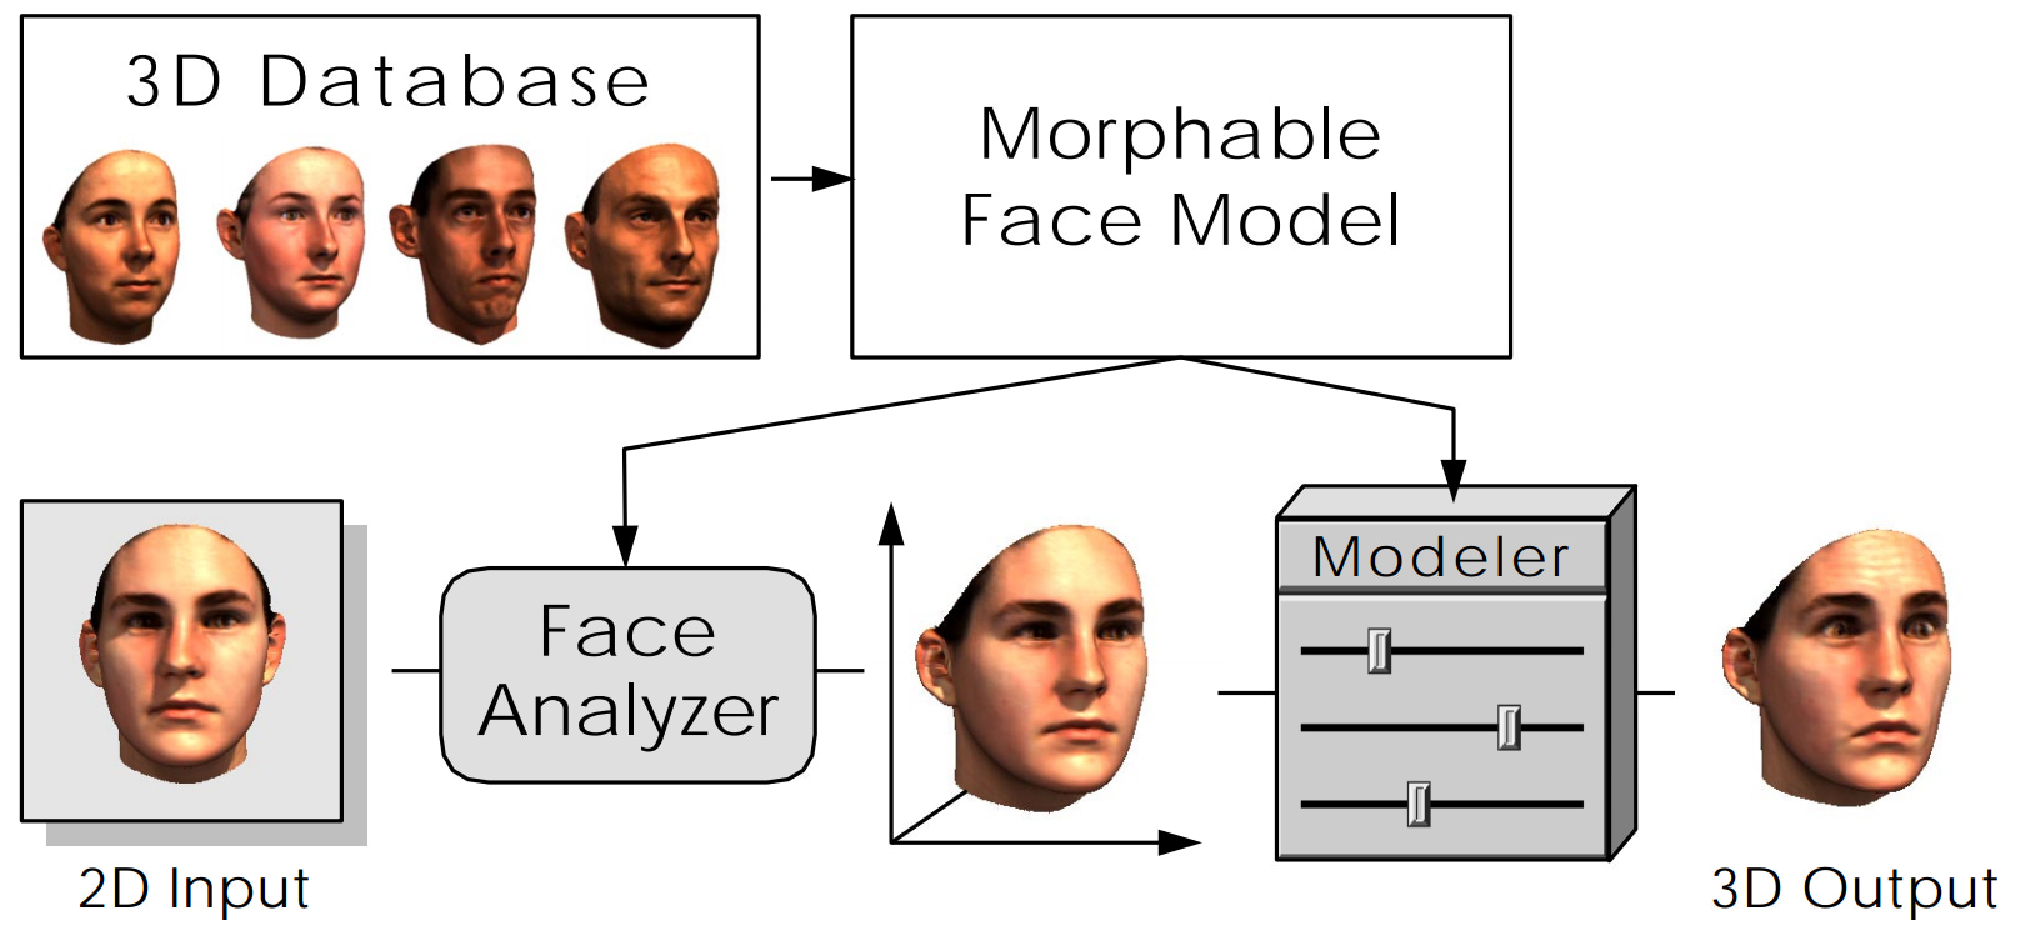
\includegraphics[width=1.0\columnwidth]{fig/img/blanz_sig99_face.pdf}
    %\vspace{-0.4cm}
    \caption{Derived from a dataset of prototypical 3D scans of faces, the morphable face model contributes to two main steps in face manipulation: (1) deriving a 3D face model from a novel image, and (2) modifying shape and texture in a natural way~\cite{Blanz:1999:MMS}.}
    \label{fig:blanz_sig99_face}
\end{figure}



\paragraph*{Morphable face.} The morphable face model~\cite{Blanz:1999:MMS} is a representative work of parametric data-driven shape reconstruction,
%Other parametric methods can be described as variants and extensions to this method.
a technique which reconstructs 3D textured faces from photos and scans. The model is learned from a dataset of prototypical 3D shapes of faces, and can then be used to derive a new 3D face from a novel image. (See Figure\ref{fig:blanz_sig99_face}).

In particular, the morphable face model represents the geometry of a face with a shape-vector $S = (\mathbf{p}_1^{T}, \cdots, \mathbf{p}_{n}^{T})^{T}) \in \mathbb{R}^{3n})$, that contains the 3D coordinates of its $n$ vertices. Similarly, it encodes the texture of a face by a texture-vector $T = (\vec{c}_1^{T}, \vec{c}_2^{T}, \cdots, \vec{c}_{n}^{T}) \in \mathbb{R}^{3n}$, that contains the RGB color values of the corresponding vertices. A morphable face model is then constructed using a database of $m$ exemplar faces, each represented by its shape-vector $S_i$ and $T_i$. In~\cite{Blanz:1999:MMS} the exemplar faces are constructed by matching a template to scanned human faces.

%Given these exemplar faces, new shapes $S_{\textup{mod}}$ and new textures $T_{\textup{mod}}$ c%an be expressed in barycentric coordinates as a linear combination of the shapes and textures:
%$$
%\vec{S}_{\textup{mod}} = \sum\limits_{i=1}^{m}a_i\vec{S}_{i} , \quad T_{\textup{mod}} = \sum\limits_{i=1}^{m}b_i\vec{T}_{i}, \quad \sum\limits_{i=1}^{m}a_i = \sum\limits_{i=1}^{m}b_i = 1.
%$$
%In other words, a morhpable model is given by the set of faces $(\vec{S}_{\textup{mod}}(\vec{a}), T_{\textup{mod}}(\vec{b}))$, parameterized by the coefficients $\vec{a} = (a_1, \cdots, %a_{m})^{T}$ and $\vec{b} = (b_1, \cdots, b_{m})^{T}$. Arbitrary new faces can be generated by varying the parameters $\vec{a}$ and $\vec{b}$ that control shape and texture.

%In addition to learning a generative model, it is important to quantify the likelihood of different regions in the parameter space. Blanz et al.~\cite{Blanz:1999:MMS} use example faces to estimate the probability distribution for the coefficients $\vec{a}$ and $\vec{b}$, which quantifies the plausibility of faces sampled from the generative model. They use
%
%Another data-driven perspective of the morphable face model is to quantify the results in terms of their plausibility of being faces. As describe in~\cite{Blanz:1999:MMS}, one way is to estimate the probability distribution for the coefficients $\vec{a}$ and $\vec{b}$ from the example faces. This distribution enables us to control the likelihood of the coefficients $\vec{a}$ and $\vec{b}$ and consequently regulate the likelihood of the appearance of the generated faces. The specific technique employed by~\cite{Blanz:1999:MMS} is
The morphable face model uses Principal Component Analysis (PCA) to characterize the shape space. A new shape and its associated texture are given by
%, which performs a basis transformation to an orthogonal coordinate system formed by the eigenvectors $\vec{s}_i$ and $\vec{t}_i$ of the covariance matrices:
$$
\vec{S}_{\textup{mod}} = \overline{\vec{S}} + \sum\limits_{i=1}^{m-1}\alpha_i \vec{s}_i, \quad \vec{T}_{\textup{mod}} = \overline{\vec{T}} + \sum\limits_{i=1}^{m-1}\beta_i \vec{t}_i,
$$
where $\overline{\vec{S}}$ and $\overline{\vec{T}}$ are the mean-shape and mean-texture, respectively, and $\vec{s}_i$ and $\vec{t}_i$ are eigenvectors of the covariance matrices. $\alpha_i$ and $\beta_i$ are coefficients. PCA also gives probability distributions over coefficients. The probability for coefficient $\alpha_i$ is given by
$$
p(\{\alpha_i\}) \sim \exp\left(-\frac{1}{2}\sum\limits_{i=1}^{m-1}(\alpha_i/\sigma_i)^2\right),
$$
with $\sigma_i^2$ being the corresponding eigenvalue of the shape covariant matrix $C_{S}$ (the probability $p(\{\beta_i\})$ is computed in a similar way).

With this morphable face model, reconstruction of textured models can be posed as a small-scale non-linear optimization problem. For example, given a 2D image of a human face $I_{\textup{input}}$, one can reconstruct the underlying textured 3D model by searching for a similar rendered face $I(\{\alpha_i\},\{\beta_i\}, p)$, parameterized by the shape and texture coefficients $\alpha_i$ and $\beta_i$, and the rendering parameters $p$ (e.g., camera configuration, lighting parameters). The optimization problem is formulated as minimizing a data term, which measures the distance between the input image and the rendered image, and regularization terms that are learned from exemplar faces. The success of the morphable model relies on the low-dimensionality of the solution space, and so is also applicable to several other data sets where this assumption holds, including the domain of human bodies and poses.

%The success of the morphable model relies on the low-dimensionality of the optimization problem, as well as the regularization terms that control the behavior of the objective function.
%Both properties are enabled have exemplar models. In the following, we discuss several other representative parametric data-driven shape reconstruction methods.

\begin{figure}[t]
\centering
    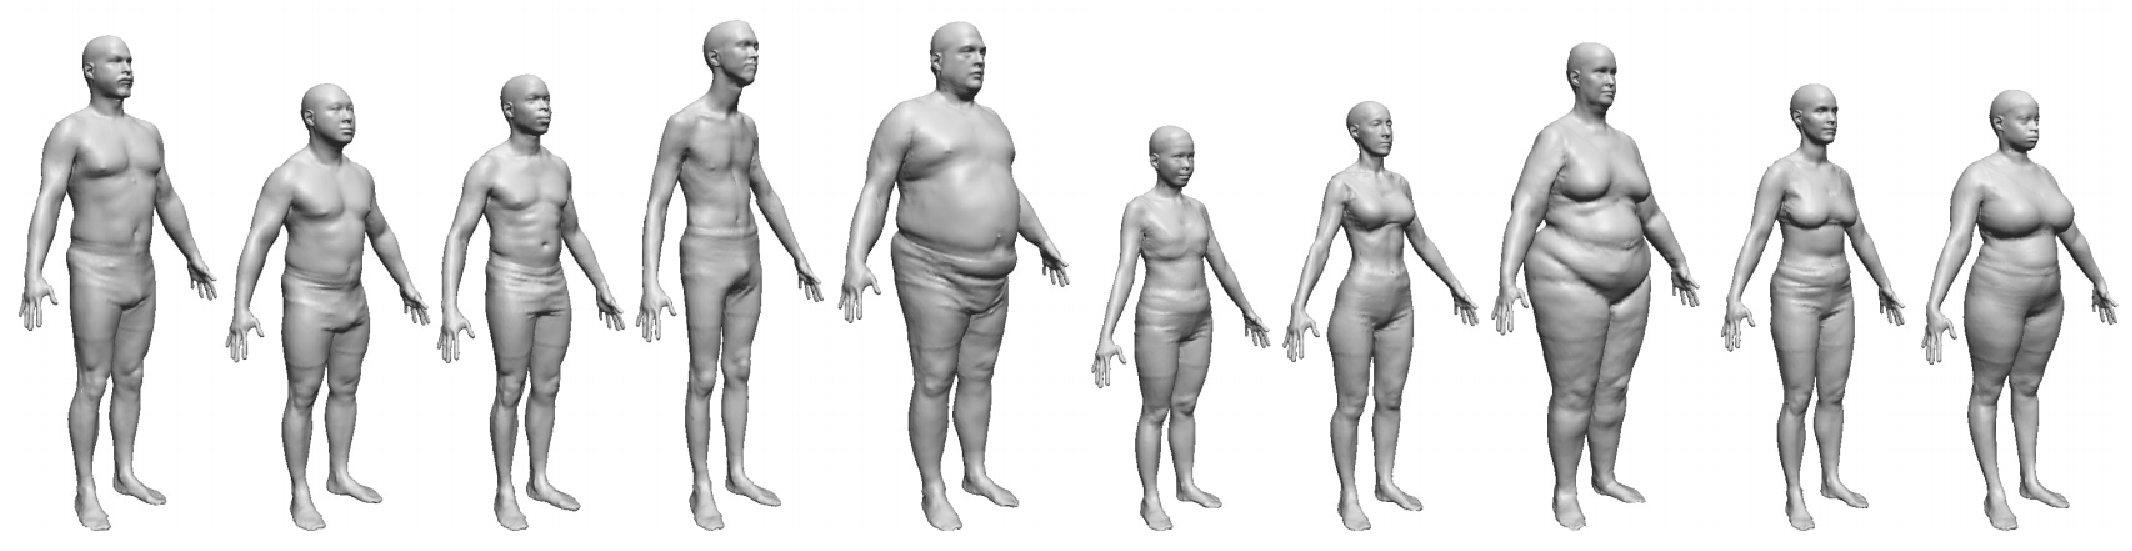
\includegraphics[width=1.0\columnwidth]{fig/img/allen_sig03_human.pdf}
    %\vspace{-0.4cm}
    \caption{Parameterizing the variation in human shapes can be used to synthesize new individuals or edit existing ones~\cite{Allen:2003:SHB}.}
    \label{fig:allen_sig03_human}
\end{figure}



\paragraph*{Morphable human bodies.} \rev{Allen et al.~\cite{Allen:2003:SHB} generalize the morphable model to characterize human bodies (Figure ~\ref{fig:allen_sig03_human}). Given a set of $250$ scanned human bodies, the method first performs non-rigid registration to fit a hole-free, artist-generated mesh (template) to each of these scans. The result is a set of mutually consistent parameterized shapes based on the corresponding vertex positions originating from the template. Similar to~\cite{Blanz:1999:MMS}, the method employs PCA to characterize the shape space, which enables applications in shape exploration, synthesis and reconstruction.}

In addition to variations in body shape, human models also exhibit variations in poses.  The SCAPE model (Shape Completion and Animation for People)~\cite{SCAPE:2005} addresses this challenge by learning two separate models of body deformation -- one accounting for variations in poses and one for differences in body shapes. The pose deformation component is acquired from a set of dense 3D scans of a single person in multiple poses. A key aspect of the pose model is that it decomposes deformation into a rigid and a non-rigid component. The rigid component is modeled using a standard skeleton system. The non-rigid component, which captures remaining deformations such as flexing of the muscles, associates each triangle with a local affine transformation matrix. These transformation matrices are learned from exemplars using a joint regression model. %Similar to previous works, SCAPE models body variations using PCA from different people in different poses.
%
In~\cite{Hasler:2009:SSR}, Hasler et al. introduce a unified model for parameterizing both shapes and poses. The basic idea is to consider the relative transformations between all pairs of neighboring triangles. These transformation matrices allow us to reconstruct the original shape by solving a least squares problem. In this regard, each shape is encoded as a set of edge-wise transformation matrices, which are fit into the PCA framework to obtain a statistical model of human shapes. The model is further extended to estimate shapes of dressed humans from range scans~\cite{Hasler:2009:TSE}.

\rev{Recent works on statistical human shape analysis focus on combining learned shape priors with sparse observations and special effects. In~\cite{Loper:SIGASIA:2014}, the authors introduce an approach that reconstructs high-quality shapes and poses from a sparse set of markers. The success of this approach relies on learning meaningful shape priors from a database consisting of thousands of shapes. In~\cite{Tsoli:2014:BLS}, the authors study human breathing from acquired data.}

% statistical human models
%\cite{}Bogo:CVPR:2014 Freifeld:2012:LBM
%\begin{figure}[t]
\centering
    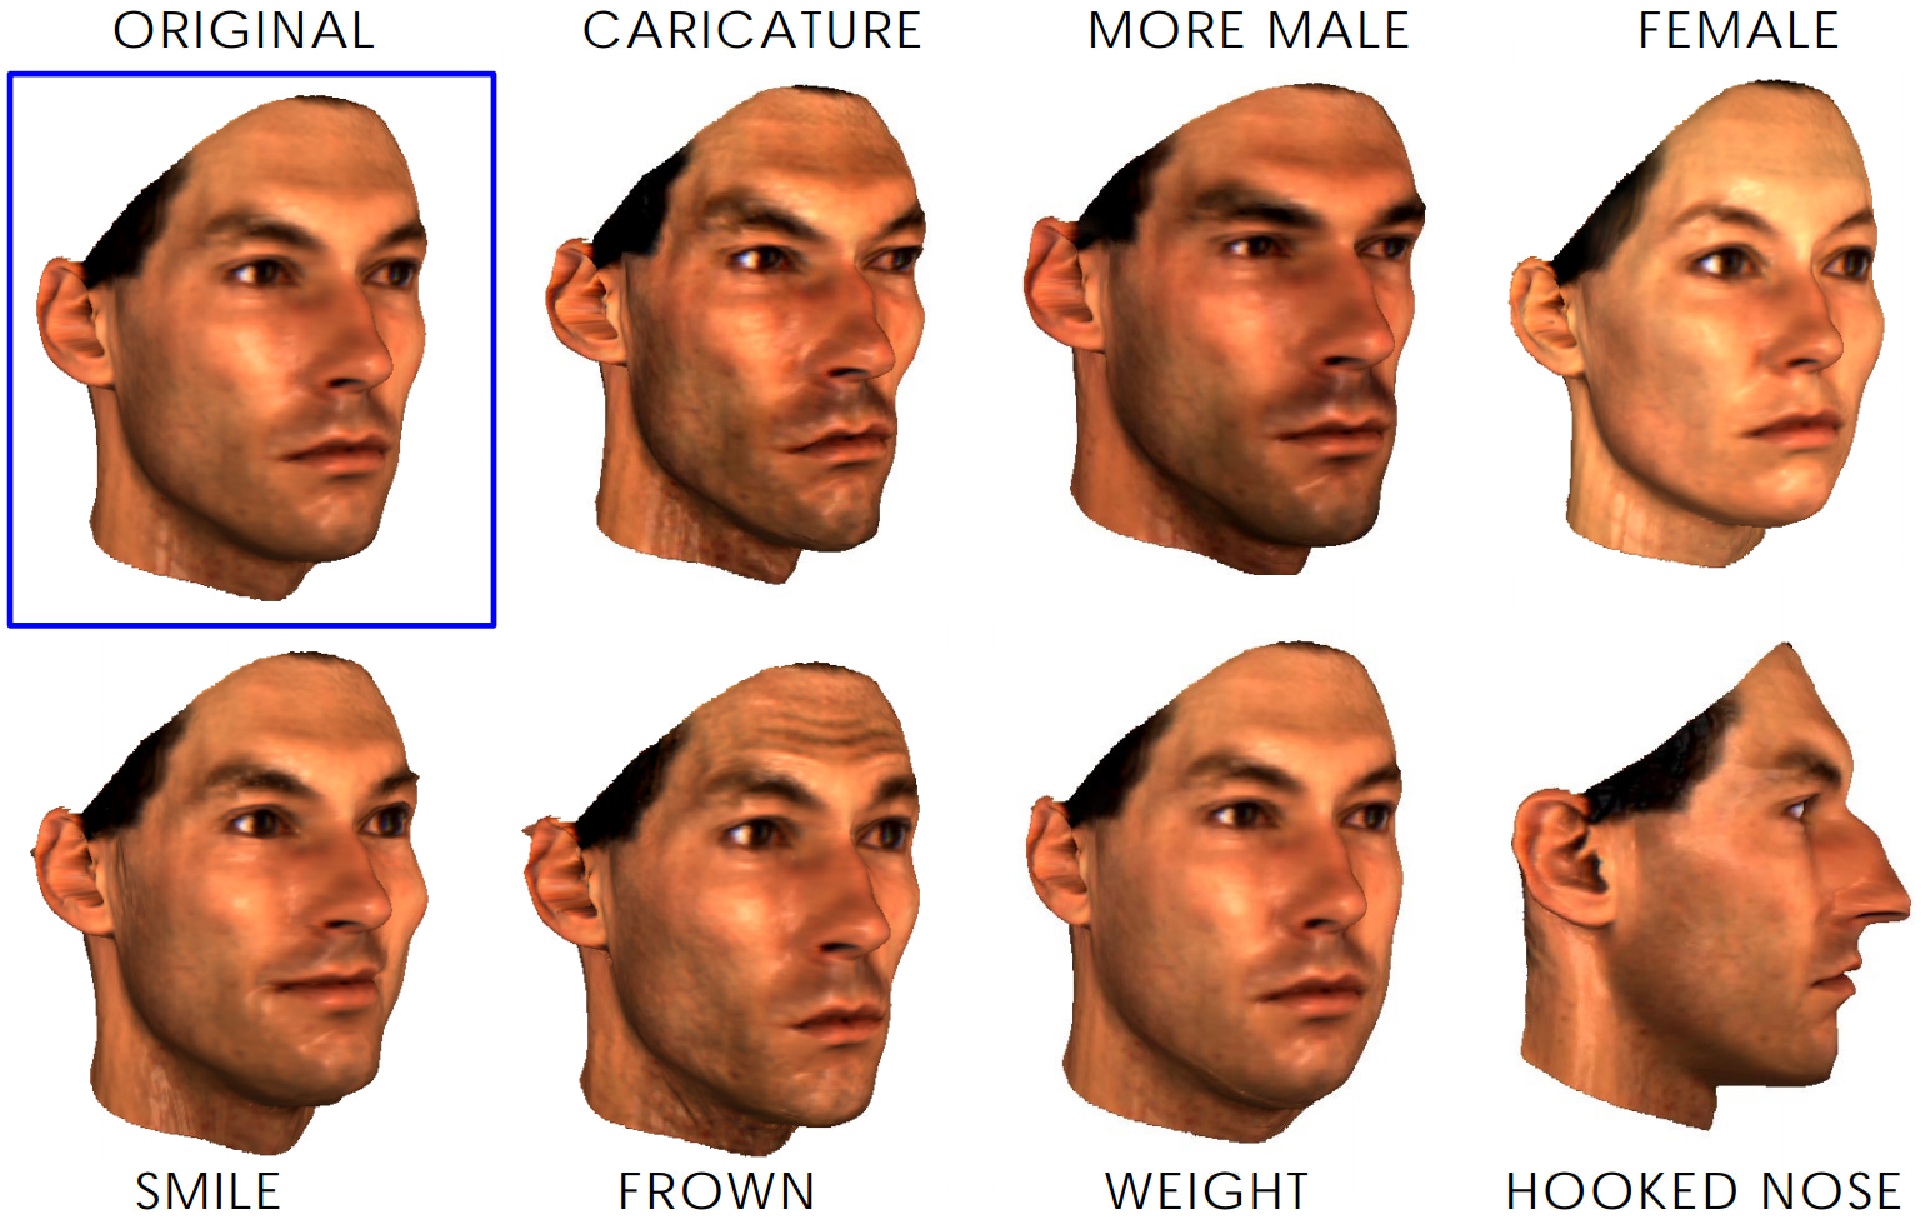
\includegraphics[width=1.0\columnwidth]{fig/img/blanz_sig99_attris.pdf}
    \vspace{-0.4cm}
    \caption{Variation of facial attributes of a single face. The appearance of the original face can be changed by adding and subtracting shape and texture vectors specific to the attribute.}
    \vspace{-0.6cm}
    \label{fig:blanz_sig99_attris}
\end{figure}


%\para{Learning shape attributes.} Besides shape reconstruction, the learned parametric shape space models can also be applied to learn shape attributes, such as facial expressions and semantic human body attributes. The morphable face model~\cite{Blanz:1999:MMS} learns facial attributes as linear combinations of positional displacements between the exemplar faces and the mean face. \cite{Li:2010:EFR} applies a similar model for face rigging.

%For human shapes existing methods~\cite{Allen:2003:SHB,SCAPE:2005,Hasler:2009:SSR} learn human body attributes such as height, weight, body fat, waist girth. Similar to faces, these attributes are described as vectors (with respect to the mean space) in the parametric shape spaces. Recently, \cite{Zhou:2010:PRH} applies these shape attributes to applications in parametric reshaping of human bodies.


\paragraph*{Data-driven tracking.} Object tracking aims to analyze dynamic shapes and/or poses of physical objects. Successful tracking techniques (e.g.,~\cite{Weise:2009:FLF,Weise:2011:RPF,Li:2013:RFA,Cao:2013:SRR,Cao:2014:DDE}) typically utilize parametric shape spaces. These reduced shape spaces provide shape priors that improve both the efficiency and robustness of the tracking process. The way to utilize and construct shape spaces vary in different settings, and are typically tailored to the specific problem setting. Weise et al.~\cite{Weise:2009:FLF} utilize a linear PCA subspace trained with a very large set of pre-processed facial expressions. This method requires an extended training session with a careful choice of facial action units. In addition, the learned face model is actor-specific. These restrictions are partially resolved in~\cite{Li:2010:EFR}, which introduces an example-based blendshape optimization technique, involving only a limited number of random facial expressions.
In~\cite{Weise:2011:RPF}, the authors combine both blendshapes and data-driven animation priors to improve the tracking performance. In a recent work, Li et al.~\cite{Li:2013:RFA} employ adaptive PCA to further improve tracking performance on nuanced emotions and micro-expression. The key idea is to combine a general blendshape PCA model and a corrective PCA model that is updated on-the-fly. This corrective PCA model captures the details of the specific actor and missing deformations from the initial blendshape model.

\vspace{-.2cm}

\subsection{Non-parametric methods}

\rev{Parametric methods require canonical domains to characterize the shape space, which have so far been demonstrated within domains of organic shapes,  such as body shapes or faces.
%, where such a canonical domain can be easily built.
%Thus, they are suitable for organic shapes such as body shapes or faces, where such a canonical domain exists. They become less effective on shapes that undergo significant geometrical and topological variations (e.g., man-made objects). \vangelis{strong statement - i do not agree that this is entirely true}
In this section, we discuss another category of methods that have shown the potential to handle more diverse shape collections.}

Generally speaking, a non-parametric data-driven shape reconstruction method utilizes a collection of relevant shapes and combines three phases, i.e., a query phase, a transformation phase and an assembly phase. Existing methods differ in how the input shape collection is preprocessed and how these phases are performed.

\begin{figure}[t]
\centering
    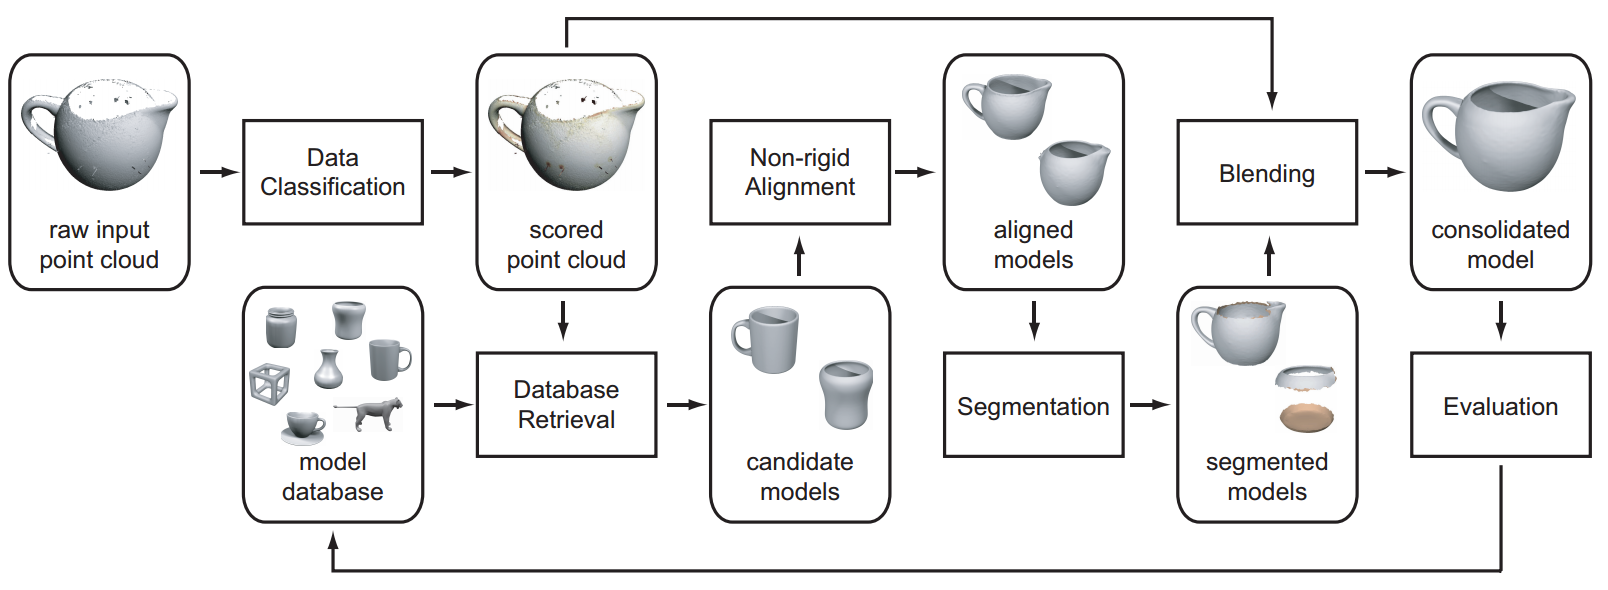
\includegraphics[width=1.0\columnwidth]{fig/img/pauly_sgp05_esr.png}
    %\vspace{-0.5cm}
    \caption{The data-driven shape reconstruction pipeline proposed in~\cite{Pauly:2005:ESC}.}
    \label{fig:pauly_sgp05_esr}
\end{figure}


\paragraph*{Example-based scan completion.} Pauly et al.~\cite{Pauly:2005:ESC} introduce one of the first non-parametric systems. As shown in~\cite{Pauly:2005:ESC}, the method takes a point cloud and a collection of complete objects as input. The reconstruction procedure incorporates all three phases described above. The first phase determines a set of similar objects. The retrieval phase combines both text-based search and PCA signatures, which are then refined by rigid alignment. The second step performs non-rigid alignment between the retrieved shapes and the input point cloud. This step partitions the input point cloud into a set of patches, where each patch is associated with one retrieved shape (via the corresponding region). The final phase merges the corresponding regions into a unified shape.

Nan et al.~\cite{Nan:2012:SAC} introduce a similar system for indoor scene reconstruction. Given an input point cloud of an indoor scene that consists of a set of objects with known categories, the method searches in a database of 3D models to find matched objects and then deforms them in a non-rigid manner to fit the input point cloud. Note that this method treats complete 3D objects as building blocks, so the final reconstruction does not necessarily reflect the original scene.
Shao et al.~\cite{Shao:2012:IAS} adopt an interactive approach to labeled segmentations of RGBD images, followed by 3D model retrieval for scene modeling. Chen et al.~\cite{Chen:2014:ASM} learn contextual relationships from a 3D scene database to further constrain the reconstruction for semantic compatibility between both objects and parts.

In contrast to considering entire 3D shapes, Gal et al.~\cite{Gal:2007:SRU} utilize a dictionary of local shape priors (defined as patches) for shape reconstruction. The method is mainly designed for enhancing shape features, where each region of an input point cloud is matched to a shape patch in the database. The matched shape patch is then used to enhance and rectify the local region. Recently, Mattausch et al.~\cite{MATTAUSCH:2014:ODC} introduce a patch-based reconstruction system for indoor scenes. Their method considers recognizing and fitting planar patches from point cloud data.

Shen et al.~\cite{Shen:2012:SRP} extends this idea for single object reconstruction by assembling object parts. Their method utilizes a collection consistently segmented 3D shapes. Given a scan of an object, the method recursively searches for parts in the collection to assemble the original object. The retrieval phase considers both the geometric similarity between the input and retrieved parts as well as part compatibility which is learned from the input shapes.
\fix{Sung et al.~\cite{Sung15} describe a framework for reliably estimating the part structure of partial scans by treating each part as a local coordinate system.
Their method also utilizes symmetric properties of the target object and shape collection, providing more accurate reconstructions on their shape completion benchmark.}


\begin{figure*}[t]
\centering
    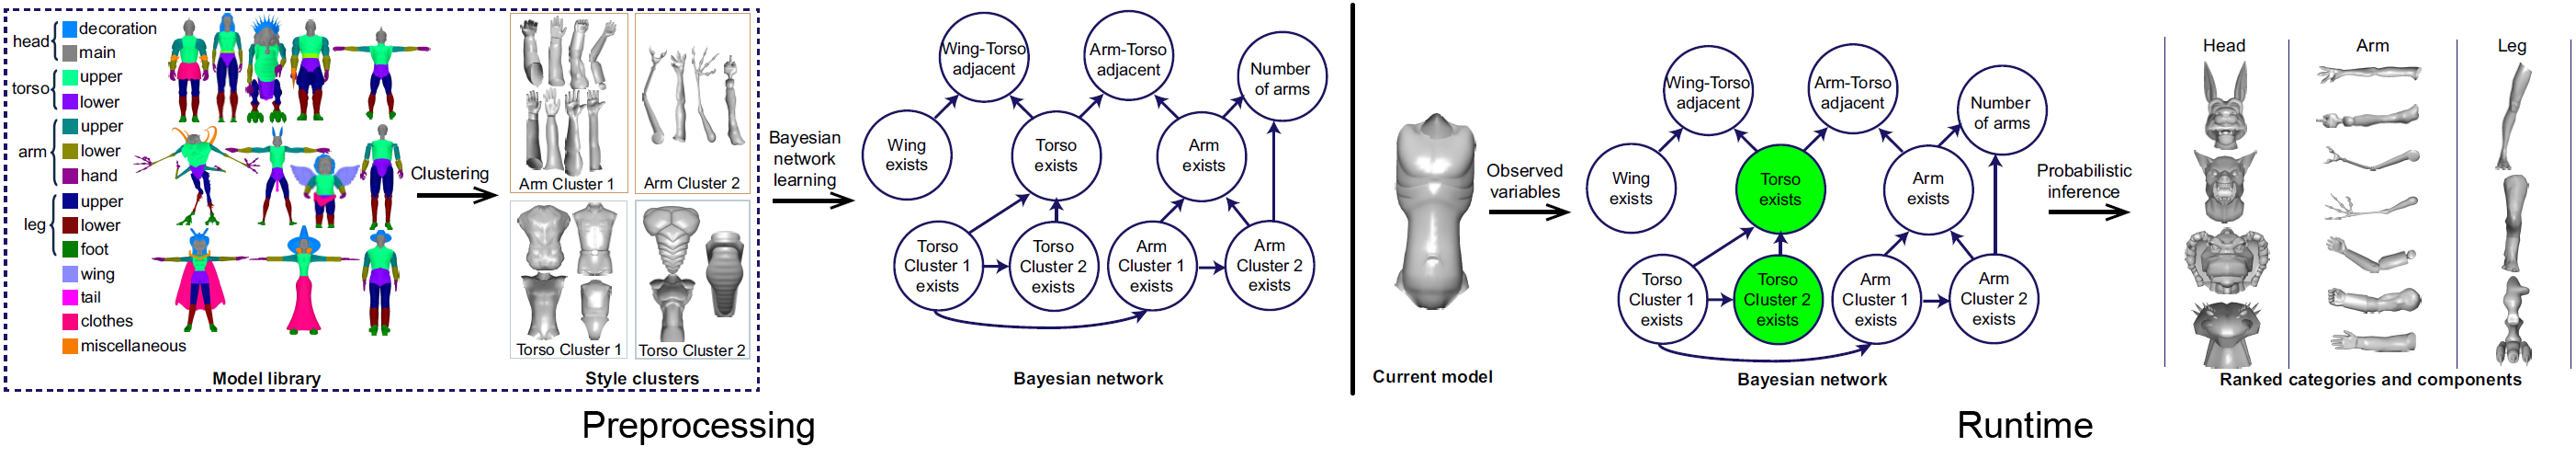
\includegraphics[width=1.0\linewidth]{fig/img/chaudhuri_sig11_prob.png}
    %\vspace{-0.4cm}
    \caption{
    Given a library of models, a Bayesian network encoding semantic and geometric relationships among shape parts
    is learned~\protect\cite{Chaudhuri:2011:prabm} (top). The modeling process (bottom) performs probabilistic inference in the learned
    Bayesian network to generate ranked lists of category labels and components within each category, customized for the currently assembled model.}
    \label{fig:segmentation_labeling}
\end{figure*}



\paragraph*{Data-driven SLAM.} Non-parametric methods have also found applications in reconstructing temporal geometric data (e.g., the output of the Kinect scanner). The Simultaneous localization and mapping (or SLAM) method is a notable technique which jointly estimates the trajectory of the scanning device along side the geometry of the environment. In this case, shape collections serve as priors for the objects in the environment, which can be used to train object detectors. For example, the SLAM++ system proposed by Salas-Moreno et al.~\cite{Salas-Moreno:2013:SLAM} trained domain specific object detectors from shape collections. The learned detectors are integrated inside the SLAM framework to recognize and track those objects. Similarly, Kim et al.~\cite{Kim:2012:AIE} use learned object models to reconstruct dense 3D models from a single scan of an indoor scene. More recently, Sun et al.~\cite{Sun:2014:SS} introduced a 3D sliding window object detector with improved performance and capability extending to a broader range of objects.
\fix{Li et al.~\cite{Li:2015:DA} propose a data-assisted online reconstruction technique which allows object retrieval from a 3D shape database while simultaneously scanning an environment in real-time.}

\paragraph*{Shape-driven reconstruction from images.} Recently, there is a growing interest in reconstructing 3D objects directly from images (e.g.,~\cite{Xu:2011:PMO,Kholgade:2014:OMS,Aubry14,Su:2014:EID}). This problem introduces fundamental challenges in both querying similar objects and deforming objects/parts to fit the input object. In terms of searching similar objects, successful methods typically render objects in the database from a dense set of viewpoints and pick objects where one view is similar to the input image object. Since depth information is missing from the image object, it is important to properly regularize 3D object transformations; otherwise, a 3D object may be deformed arbitrarily even though its projection on the image domain matches the image object. Most existing techniques consider rigid transformations or user-specified deformations~\cite{Xu:2011:PMO}. In a recent work, Su et al.~\cite{Su:2014:EID} propose to learn meaningful deformations of each shape from its optimal deformation to similar shapes.
\fix{Huang et al.~\cite{Huang:SVR:2015} jointly analyze a large collection of images in object categories and a smaller collection of 3D models
to achieve simultaneous analysis and reconstruction of 2D images.}

%\subsection{Discussion and Future directions}

%Despite the progress made in data-driven shape reconstruction, this problem is far-from being solved. The key challenge in parametric methods is to obtain consistently correspondences across the shapes. Existing techniques typically utilize template matching and require a significant amount of manual interaction, which limit them to small-scale datasets (e.g., hundreds of shapes). With the availability large geometric data, it is necessary to scale-up the learning phase of parametric methods, since learning from large shape data would result in more accurate statistics and thus provide better priors for reconstruction. Another challenge of parametric methods is to constrain the shape space so that it avoids infeasible shapes. This is the fundamental limitation of linear shape space methods. One way to address this issue is to perform sampling of feasible shapes (c.f.,~\cite{Wang:2009:RHC}). While it is demanding to develop to alternative ways to characterize shape spaces.

%For non-parametric methods, there is a fundamental tradeoff between the efficiency of shape retrieval and having a large shape collection so that one can always find similar shapes for the object of consideration. Just as what have been done images, developing effective tools that index through 3D shapes plays a central role here. In addition, in many cases the retrieval object/part is similar in global shape but differ in local details to the underlying object. Thus, another challenge of non-parametric methods is how to recover shape details of the underlying object. Note that this problem cannot be resolved by simply deforming the retrieval objects.

%It would be very interesting to extend parametric methods to man-made shapes. A potential direction to explore is to learn shape grammars from shape collections. However, this problem is quite challenging as we have to resolve obstacles in both defining the grammar and learning grammar from shape collections.

%It would be intersting
%There is a fundamental tradeoff for non-parametric methods --- the efficiency in shape retrieval   


\section{Shape modeling and synthesis}
\label{sec:modeling}

So far, the creation of detailed three-dimensional content remains a tedious task which can mainly be performed by skilled artists.
3D content creation has been a major bottleneck hindering the development of ubiquitous 3D graphics.
Thus, providing easy-to-use tools for casual and novice users to design and create 3D models has been a key
challenge in computer graphics. To address this challenge, current literature has been focused on two main directions, i.e.,
intelligent interfaces for interactive shape modeling and smart models for automated model synthesis.
%The former strives to endow a modeling interface with a higher-level understanding of the structure and semantics of 3D shapes, allowing the interface to reason around the incomplete shape being modeled~\cite{Chaudhuri:2010:DDS}.
%
%The second direction follows the modeling-by-example paradigm~\cite{Funkhouser:2004:MBE}.
%The second direction follows the by-example synthesis paradigm.
%Given a set of semantically related shapes, the goal is to generate more shapes which are both novel and plausible.
%This can be approached by several models, such as generative models~\cite{Allen:2003:SHB},
%evolutionary computation~\cite{Sims:1991:AE}, and inverse procedural modeling~\cite{Stava:2010:IPM}.
The former strives to endow modeling interfaces with a higher-level understanding of the structure and semantics
of 3D shapes, allowing the interface to reason around the incomplete shapes being modeled. The latter direction focuses on developing data-driven models to synthesize new shapes automatically.
%The core problem is to learn from the input shape set a model that encapsulates
%geometric, structural and functional constraints to drive the automatic synthesis of novel shapes.
The core problem is to learn generative shape models from a set of exemplars (e.g., probability distributions, fitness functions, functional constraints, etc) so that the synthesized shapes are plausible and novel.
It can be seen that both of the two paradigms depend on data-driven modeling of shape structures and semantics.
With the availability of large 3D shape collections, the data-driven approach becomes a promising answer to the content creation bottleneck.

\subsection{Interactive shape modeling and editing}
\label{sec:interactive_modeling}
%Interactive modeling is perhaps the most prevailing manner of designing and creating 3D models, as
%reflected by the highly matured modeling softwares (3DS Max, Maya, etc.).
Interactive 3D modeling software (3DS Max, Maya, etc.) provide artists with a large set of tools
for creating and editing detailed 3D models.  Unfortunately, this same software is often onerous to harness for non-professional users.
For casual users, more intuitive modeling interfaces with a certain machine intelligence are to be preferred. Below, we discuss such methods for assembly-based modeling and guided shape editing.

%\vangelis{it is ok, we discuss this high-level understanding many times in the text already}
%The key to making interactive modeling more accessible is to equip the interfaces with a higher-level understanding of the structure and semantics of 3D shapes, so that they can reason about the partially modeled shapes, to enhance the modeling process with useful suggestions, informative guidance and smart automation.

\paragraph*{Assembly-based modeling.}
Early works on 3D modeling based on shape sets are primarily driven by the purpose of \emph{content reuse}
in part-assembly based modeling approaches.
The seminal work of modeling by example~\cite{Funkhouser:2004:MBE} presents a pioneering system
of shape modeling by searching a shape database for parts to reuse in the construction of new shapes.
Kraevoy et al.~\shortcite{Kreavoy:2007:MIC} describe a system for shape creation
via interchanging parts between a small set of compatible shapes.
Guo et al.~\cite{Guo:2014:CG} propose assembly-based creature modeling guided by a shape grammar.

\rev{Beyond content reuse through database queries or hand-crafted rules, Chaudhuri and Koltun~\shortcite{Chaudhuri:2010:DDS} propose a data-driven technique
for suggesting the modeler with shape parts that can potentially augment the current shape being built.}
Such part suggestions are generated through retrieving a shape from a database based on partial shape matching.
Although this is a purely geometric method without accounting for the semantics of shape parts,
it represents the first attempt at utilizing a shape database to \emph{augment the modeling interface}.
Later, Chaudhuri et al.~\shortcite{Chaudhuri:2011:prabm} show that the incorporation of
semantic relationships increases the relevance of presented parts.
Given a repository of 3D shapes, the method learns a probabilistic graphical model encoding semantic and geometric
relationships among shape parts. During modeling, inference in the learned Bayesian network
is performed to produce a relevance ranking of the parts.

A common limitation of the above techniques is that they do not provide a way to directly express a high-level design goal (e.g. ``create a cute toy''). Chaudhuri et al.~\shortcite{Chaudhuri:2013:ACC} proposed a method that learns semantic attributes for shape parts that reflect the high-level intent people may have for creating content in a domain (e.g. adjectives such as ``dangerous'', ``scary'' or ``strong'') and ranks them according to the strength of each learned attribute (Figure \ref{fig:attribit}). During an interactive session, the user explores and modifies the strengths of semantic attributes to generate new part assemblies.

3D shape collections can supply other useful information as well, such as contextual and spatial relationships between shape parts,
to enhance a variety of modeling interfaces.
Xie et al.~\cite{Xie:2013:S2D} propose a data-driven sketch-based 3D modeling system.
In the off-line learning stage, a shape database is pre-analyzed to extract the contextual information among parts.
During the online stage, the user designs a 3D model by progressively sketching its parts and retrieving and assembling
shape parts from the database. Both the retrieval and assembly are assisted by
precomputed contextual information so that more relevant parts can be returned and selected parts can be automatically placed.
Inspired by the ShadowDraw system~\cite{Lee:2011:SD}, Fan et al.~\cite{Fan:2013:MBD} propose 3D modeling by drawing with
data-driven shadow guidance. The user's strokes are used to query a 3D shape database for generating the shadow image,
which in turn can guide the user's drawing. Along the drawing, 3D candidate parts are retrieved for assembly-based modeling.
\fix{
Starting from a collection of expertly-created, fabricable 3D models, Schulz et al.~\cite{Schulz:2014:DFE} extract
parameterized design templates encoding all information necessary for fabrication.
The templates can then be used to generate new fabricable models in an interactive design system.
}


\paragraph*{Shape editing.}
The general idea of data-driven shape editing is to learn a model from a collection of closely related shapes
that characterizes the plausible variations or deformations of the shapes in this collection.  In this way, the learned model
can be used to constrain a user's edit to maintain plausibility.
For organic shapes, such as human faces~\cite{Blanz:1999:MMS,Chen:2014:FED} or bodies~\cite{Allen:2003:SHB},
parametric models can be learned from a shape set characterizing its shape space.
Such parametric models can be used to edit the shapes through exploring the shape space with the set of parameters.

%For man-made shapes, however, learning such parametric shape space is intractable since their plausibility is related with structure~\cite{Mitra:2014:SASP}.
% \vangelis{structure can be parametrized as well}
An alternative widely-adopted approach is the analyze-and-edit paradigm.  This technique first extracts the structure of the input shape, and then uses this structure to constrain the editing phase to be more tenable~\cite{Gal:2009:IAA}.
Instead of learning structure from a single shape, Fish et al.~\cite{Fish:2014:MR} learn it from a set of shapes that belong to the same family, resulting in a set of probability distributions characterizing the part arrangements. These distributions can be used to guide structure-preserving editing, where models can be
edited while maintaining their familial traits.
Yumer et al.~\cite{Yumer:2014:CCH} extract co-constrained handles from a set of shapes for shape deformation.
The handles are generated based on co-abstraction~\cite{Yumer:2012:CSC} of the set of shapes and the deformation co-constraints are learned statistically from the set. \rev{The deformation handles can also be controlled with continuous semantic attributes \cite{Yumer:2015:SSE}.} \revnew{This approach also benefit from deep neural network trained to predict appropriate deformations for 3D models~\cite{yumer2016learning}.}

Based on learned structures from a database of 3D models, Xu et al.~\cite{Xu:2011:PMO} propose photo-inspired 3D object modeling.
Guided by the object in a photograph, the method creates a 3D model as a geometric variation of a candidate model retrieved from the database.
Due to the pre-analyzed structural information, the method addresses the ill-posed problem of 3D modeling from a single 2D image
via structure-preserving 3D warping. The final result is structurally plausible and is readily usable for subsequent editing.
Moreover, the resulting 3D model, although built from a single view, is structurally coherent from all views.

\subsection{Automated synthesis of shapes}
\label{sec:synthesis}
\begin{figure}[t]
\centering
    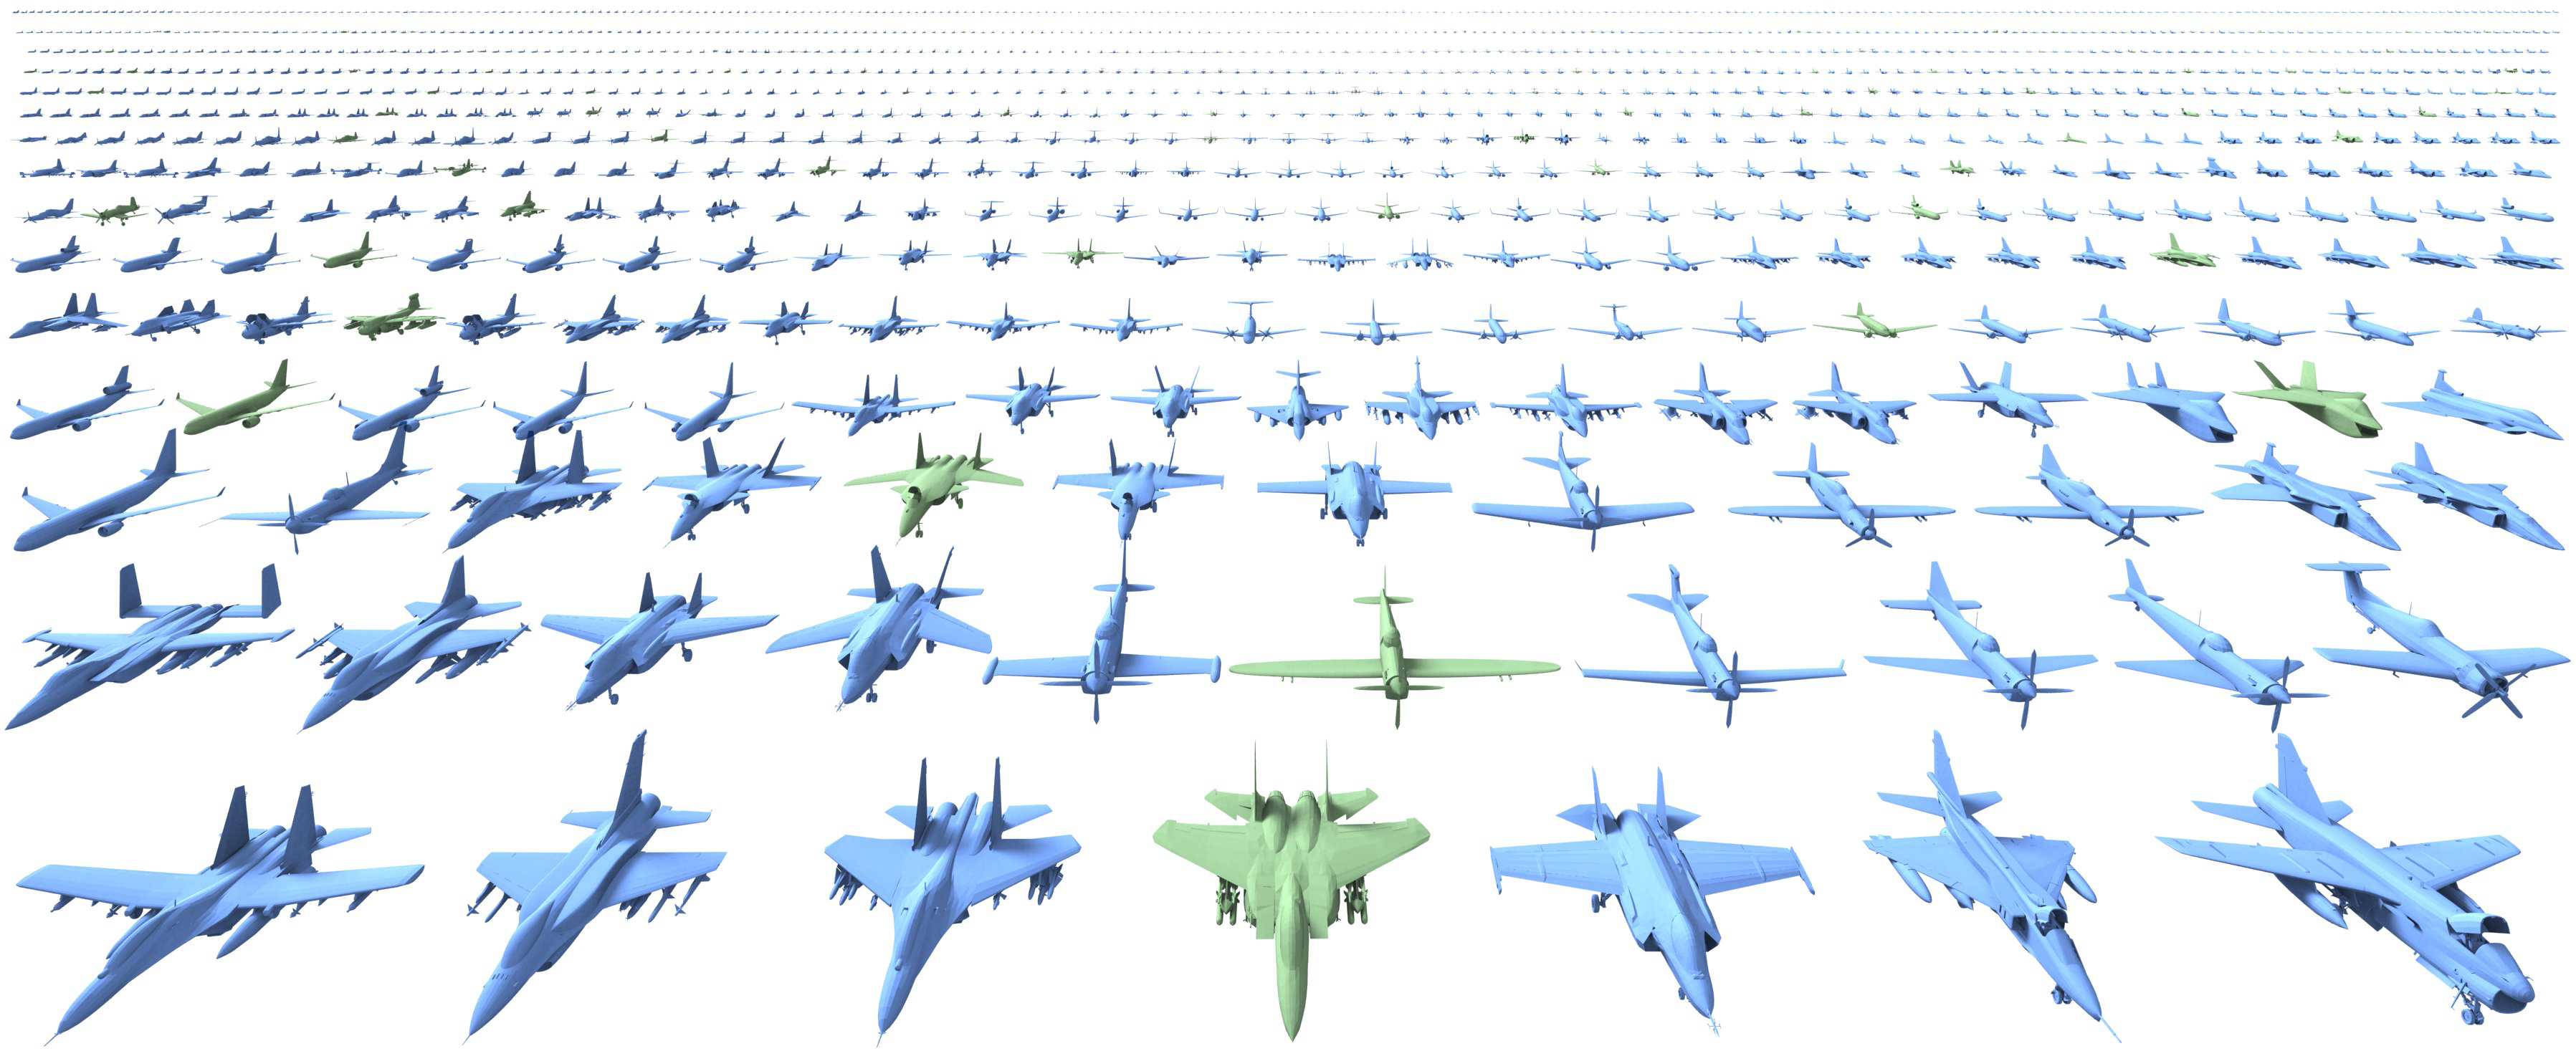
\includegraphics[width=.95\columnwidth]{fig/img/kalogerakis_sig12_synthesis}
    %\vspace{-0.3cm}
    \caption{
Given a hundred training airplanes (in green), the probabilistic model from \cite{Kalogerakis:2012:PMC} synthesizes several hundreds of new airplanes (in blue).}
    \label{fig:kalogerakis_sig12_synthesis}
\end{figure}



\rev{Many applications such as 3D games and films require large collections of 3D shapes for populating their environments. Modeling each shape individually can be tedious even with the best interactive tools. The goal of data-driven shape synthesis algorithms is to generate several shapes automatically with no or very little user supervision: users may only provide some preferences or high-level specifications to control the shape synthesis process. Existing methods achieve this task by using probabilistic generative models of shapes, evolutionary methods, or learned probabilistic grammars.}

\paragraph*{Statistical models of shapes.} The basic idea of these methods is to define a parametric shape space and then fit a probability distribution to the data points that represent the input exemplar shapes. Since the input shapes are assumed to be plausible and desired representatives of the shape space, high-probability areas of the shape space which tend to become associated with new, plausible shape variants. \rev{ This idea was first explored in the context of parametric models \cite{Blanz:1999:MMS,Allen:2003:SHB}, discussed in Section \ref{sec:recon}. By associating each principal component of the shape space defined by these methods with a Gaussian distribution, this distribution can be sampled to generate new human faces or bodies (Figure \ref{fig:allen_sig03_human}). Since the probability distribution of plausible shapes tends to be highly non-uniform in several shape classes, Talton et al. \cite{Talton:2009:EMC} use kernel density estimation with Gaussian kernels to represent plausible shape variability. The method is able to generate new shapes for tree and human body parametric spaces. }

Shapes have structure i.e., shapes vary in terms of their type and style, different shape styles have different number and type of parts, parts have various sub-parts that can be made of patches, and so on. Thus, to generate shapes in complex domains, it is important to define shape spaces over structural and geometric parameters, and capture hierarchical relationships between these parameters at different levels. Kalogerakis et al. \cite{Kalogerakis:2012:PMC} (Figure \ref{fig:kalogerakis_sig12_synthesis}) proposed a probabilistic model that represents variation and relationships of geometric descriptors and adjacency features for different part styles, as well as variation and relationships of part styles and repetitions for different shape styles. The method learns the model from a set of consistently segmented shapes. Part and shape styles are discovered based on latent variables that capture the underlying modes of shape variability. The method uses a search procedure to assemble new shapes from parts of the input shapes according to the learned probability distribution. Users can also set preferences for generating shapes from a particular shape style, with given part styles or specific parts. \fix{Instead of relying on pre-segmented shapes and high-level part descriptors to encode shape variability, Huang et al. \cite{Huang:2015:AS3} propose a probabilistic model that jointly estimates shape segmentation, surface correspondences, and surface descriptors from an input shape dataset. A deep learning procedure was used to capture hierarchical relationships of corresponding surface point positions and parts as well as their existence in the input shapes. Their probabilistic model can be sampled to directly generate point-sampled surface geometry and shape structure.}

\paragraph*{Set evolution.} \rev{Xu et al. \cite{Xu:FDS:2012} developed a method for generating shapes inspired by the theory of evolution in biology.} The basic idea of set evolution is to define cross-over and mutation operators on shapes to perform part warping and part replacement. Starting from an initial generation of shapes with part correspondences and built-in structural information such as inter-part symmetries, these operators are applied to create a new generation of shapes. A selected subset from the generation is presented via a gallery to the user who provides feedback to the system by rating them. The ratings are used to define the fitness function for the evolution. Through the evolution, the set is personalized and populated with shapes that better fit to the user. At the same time, the system explicitly maintains the diversity of the population so as to prevent it from converging into an ``elite'' set.

\paragraph*{Learned shape grammars.} Talton et al. \cite{Talton:2012:LDP} leverage techniques
from natural language processing to learn probabilistic generative grammars of shapes. The method takes as input a set of exemplar shapes represented with a scene graph specifying parent/child relationships and
relative transformations between labeled shape components. They use Bayesian inference to learn a probabilistic formal grammar that can be used to synthesize novel shapes. 



%\input{joint}

\section{Scene analysis and synthesis}
\label{sec:scene}
% motivation
Analyzing and modeling indoor and outdoor environments has important applications in various domains. For example, in robotics it is desirable for an autonomous agent to understand the semantics of 3D environments to be able to interact with them. In urban planning and architecture, professionals build digital models of cities and buildings to validate and improve their designs. In computer graphics, artists create novel 3D scenes for movies and video games.


%\teaser{
\begin{figure}[t]
\centering
    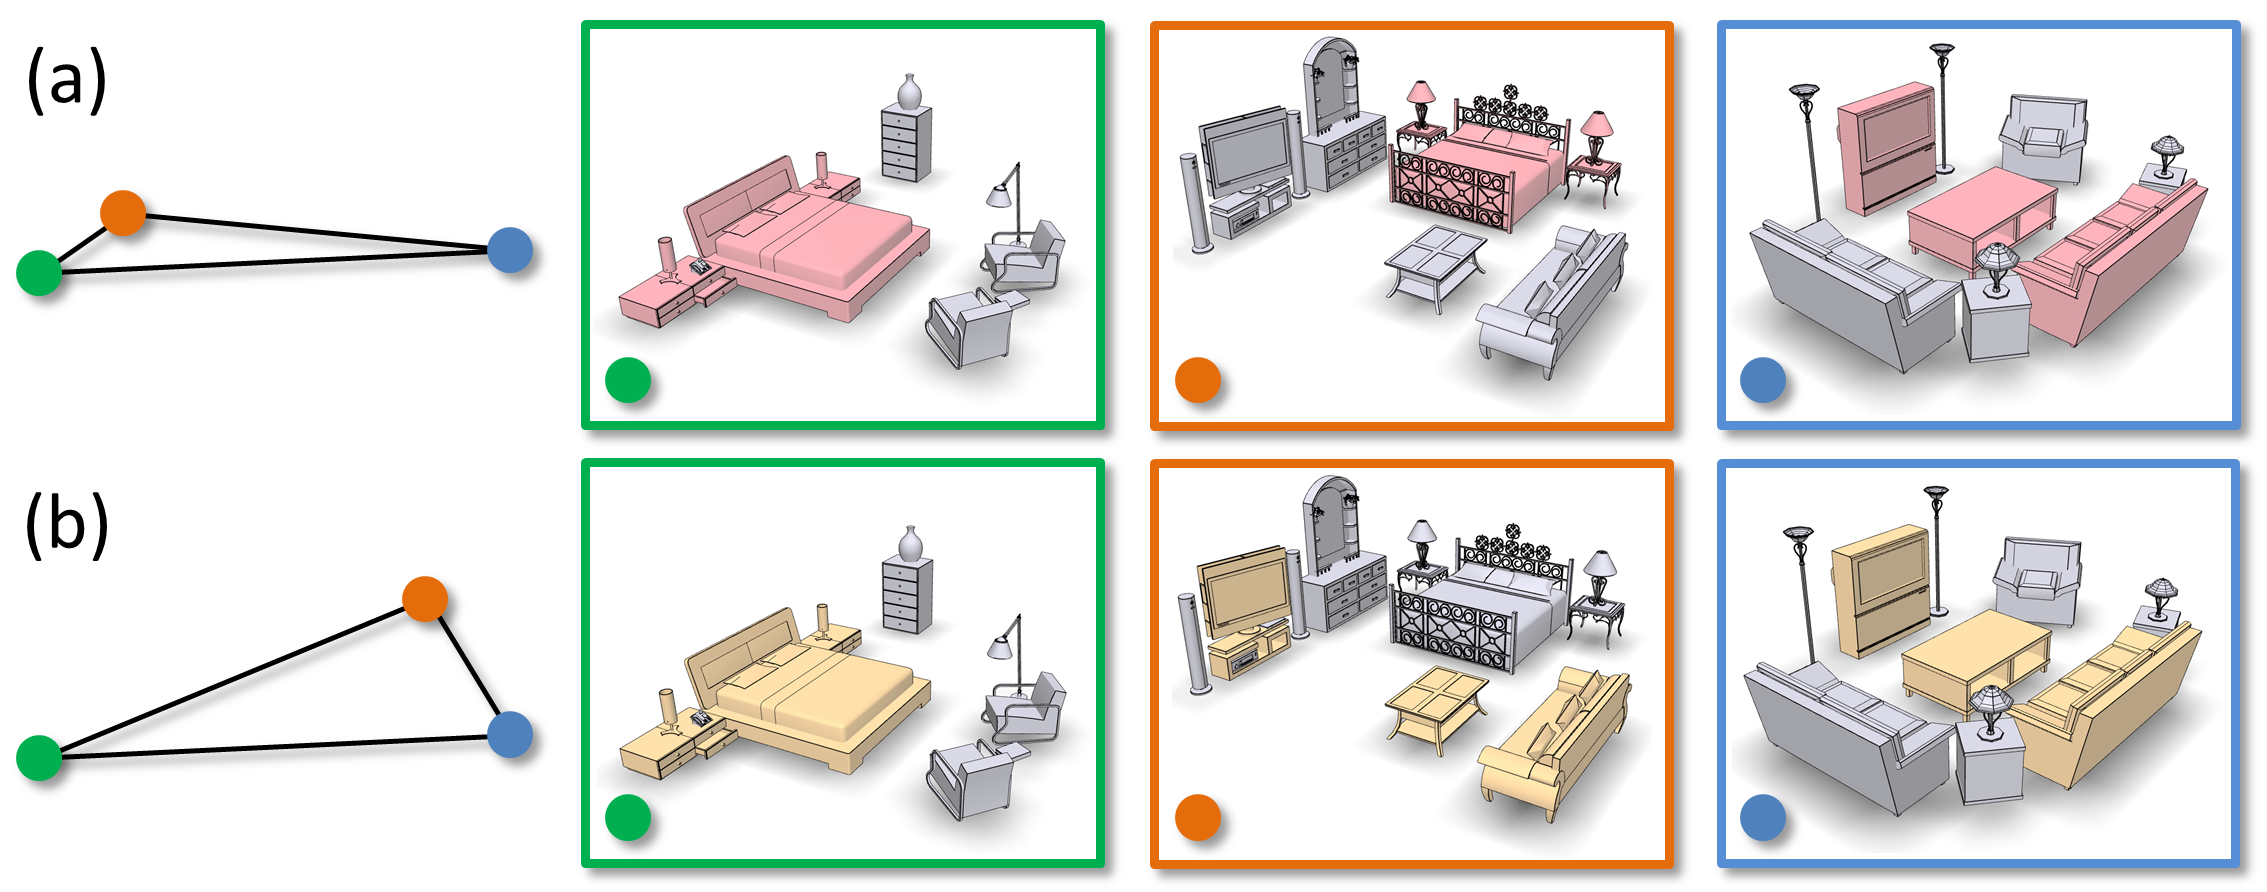
\includegraphics[width=0.99\linewidth]{fig/img/xu_sig14_focal}
    %\vspace{-0.2cm}
    \caption{
    Scene comparisons may yield different similarity distances (left) depending on the focal points~\cite{Xu:2014:OHSC}.}
    \label{fig:xu_sig14_focal}
\end{figure}
%}


% opportunities and challenges
The fast growing number of 3D scenes in digital repositories provide new opportunities for data-driven scene analysis, editing, and synthesis. Emerging collections of 3D scenes pose novel research challenges that cannot be easily addressed with existing tools.  In particular, representations created for analyzing collections of single models mostly focus on arrangement and relations between shape parts~\cite{Mitra:2014:SASP}, which usually exhibit less variations than objects in scenes. Capturing scene structure poses a greater challenge due to looser spatial relations and a more diverse mixture of functional substructures.

%
%The analysis of model collections has been prevalently focused on single objects.
%where the main focus of study is the arrangement and relations between shape parts, and their connection with functionality or semantics~\cite{Mitra:2014:SASP}.
%Compared to the structure of shape parts in a single object, the structural layout of objects in a scene is more complex due to the looser spatial relations and a more diverse mixture of functional substructures.

% previous work on image understanding
Inferring scene semantics is a long-standing problem in image understanding, with many methods developed for object recognition~\cite{quattoni2009}, classification~\cite{swadzba2010},
layout and structure reasoning~\cite{Choi:2013:UIS,Fouhey:2013:DDP} with \emph{a single image}. Previous work demonstrates that one can leverage collections of 3D models to facilitate scene understanding in images~\cite{Satkin:2012:DDS}.
In addition, the depth information in RGBD scans can be used to establish the link between 2D and 3D for model-driven scene understanding~\cite{Silberman:2012:ISS}. The semantic annotations of images are not immediately useful for modeling and synthesizing 3D scenes, for which the geometric and structural priors have to be learned from 3D data.

In this section, we cover the data-driven techniques that leverage collections of 3D scenes for modeling, editing, and synthesizing novel scenes.

%In this section, we will mainly cover works on scene analysis and synthesis
%from the graphics community, with the main focus on 3D indoor scenes.

\paragraph*{Context-based retrieval.}
To address the large variation in the geometry and arrangement of objects in scenes, Fisher et al.~\cite{Fisher:2010:CSM,Fisher:2011:CSR} propose to take advantage of local context.  One of the key insights of their work is that collections of 3D scenes provide rich information about context in which objects appear. They show that capturing these contextual priors can help in scene retrieval and editing.

Their system takes an annotated collection of 3D scenes as input, where each object in a scene is classified. They represent each scene as a graph, where nodes represent objects and edges represent relations between objects, such as support and surface contact. In order to compare scenes, they define kernel functions for pairs of nodes measuring similarity in object geometry, and for pairs of edges, measuring similarity in relations of two pairs of objects.  They further define a graph kernel to compare pairs of scenes.  In particular, they compare all walks of fixed length originating at all pairs of objects in both scene graphs, which loosely captures similarities of all contexts in which objects appear~\cite{Fisher:2011:CSR}.  They show that this similarity metric can be used to retrieve scenes. By comparing only paths originated at a particular object, they can retrieve objects for interactive scene editing.

%Their scene editing interface also allows retrieving relevant models by placing bounding boxes into partially modeled scenes, where the system returns a most relevant object that conforms to box dimensions and contextual relationship to the surrounding objects~\cite{Fisher:2010:CSM}.


%model spatial relationship between pairs of objects using kernel density estimation~\cite{Fisher:2010:CSM}. Such learned spatial relationship can be used in context-based object retrieval, which can be quite effective in assisting interactive scene modeling. For example, the user places a bounding box into the partially modeled scene as a proxy and the system can return a relevant object which both conforms to the size of the proxy and admits the contextual relationship against the surrounding objects.
%
%Later, Fisher et al. propose the first similarity measure for 3D scenes through
%representing scenes as graphs which encode models and their contextual relationships and then
%defining a kernel between the relationship graphs~\cite{Fisher:2011:CSR}.
%Such graph kernel based scene similarity is shown to be discriminative for scene retrieval.
%Meanwhile, since the graph kernel integrates spatial relationships between all objects in the scene,
%it is also informative in characterizing contextual information and outperforms their previous method~\cite{Fisher:2010:CSM}
%for context-based object retrieval.



\paragraph*{Focal points.}
Measuring the similarity of complex hybrid scenes such as studios composed of a bedroom, living room, and dining room poses a challenge to graph kernel techniques since they only measure global scene similarity. Thus, Xu et al.~\shortcite{Xu:2014:OHSC} advocate analyzing salient sub-scenes, which they call focal points, to compare hybrid scenes, i.e., scenes containing multiple salient sub-scenes. Figure~\ref{fig:xu_sig14_focal} shows an example of comparing complex scenes, where
the middle scene is a hybrid one encompassing two semantically salient sub-scenes, i.e., bed-nightstands and TV-table-sofa.
The middle scene is closer to the left one when the bed and nightstands are focused on, and otherwise when the TV-table-sofa combo is the focal point.
Therefore, scene comparison may yield different similarity distances depending on the focal points.

Formally, a focal point is defined as a representative substructure of a scene which can characterize a semantic scene category. That means the substructure should re-occur frequently only within that category. Therefore, focal point detection is naturally coupled with the identification of scene categories via scene clustering. This poses coupled problems of detecting focal points based on scene groups and grouping scenes based on focal points.
These two problems are solved via interleaved optimization which alternates between focal point detection and focal-based scene clustering. The former is achieved by mining frequent substructures and the latter uses subspace clustering, where scene distances are defined in a focal-centric manner.  Inspired by the work of Fisher et al.~\cite{Fisher:2011:CSR}, scene distances are computed using focal-centric graph kernels which are estimated from walks originating from representative focal points.


\begin{figure}[t] \centering
    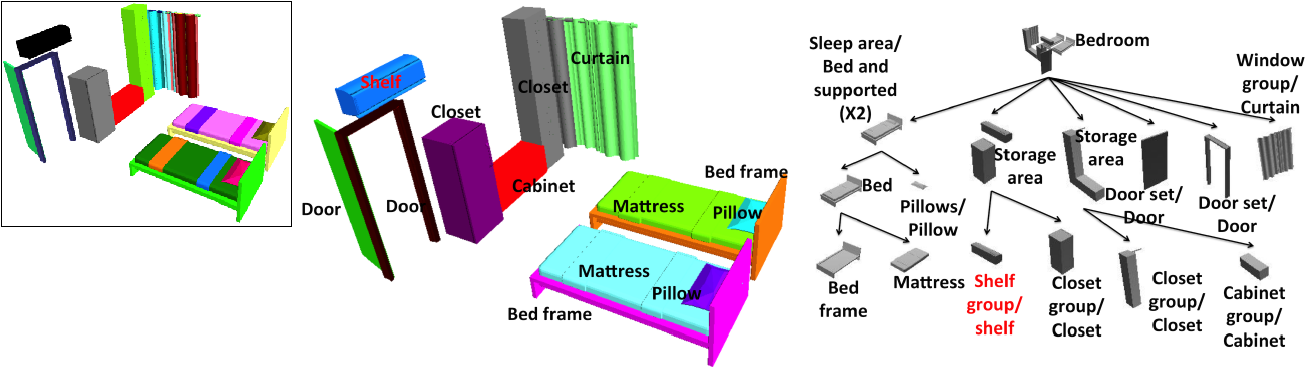
\includegraphics[width=0.98\linewidth]{fig/img/liu_siga14_sh}
        %\vspace{-0.3cm}
    \caption{
    The algorithm processes raw scene graphs with possible over-segmentation (a) into consistent hierarchies capturing semantic and functional groups (b,c)~\cite{Liu:2014:CCS}.
    }
    \label{fig:liu_siga14_sh}
\end{figure}


%
The detected focal points can be used to organize the scene collection and to support efficient exploration of the collection (see Section~\ref{sec:exploration}). Focal-based scene similarity can be used for novel applications such as multi-query scene retrieval,
where one may issue queries consisting of multiple semantically related scenes and wish to retrieve more scenes ``of the same kind''.% (Figure~\ref{fig:multiquery}).

%
\begin{figure}[t] \centering
    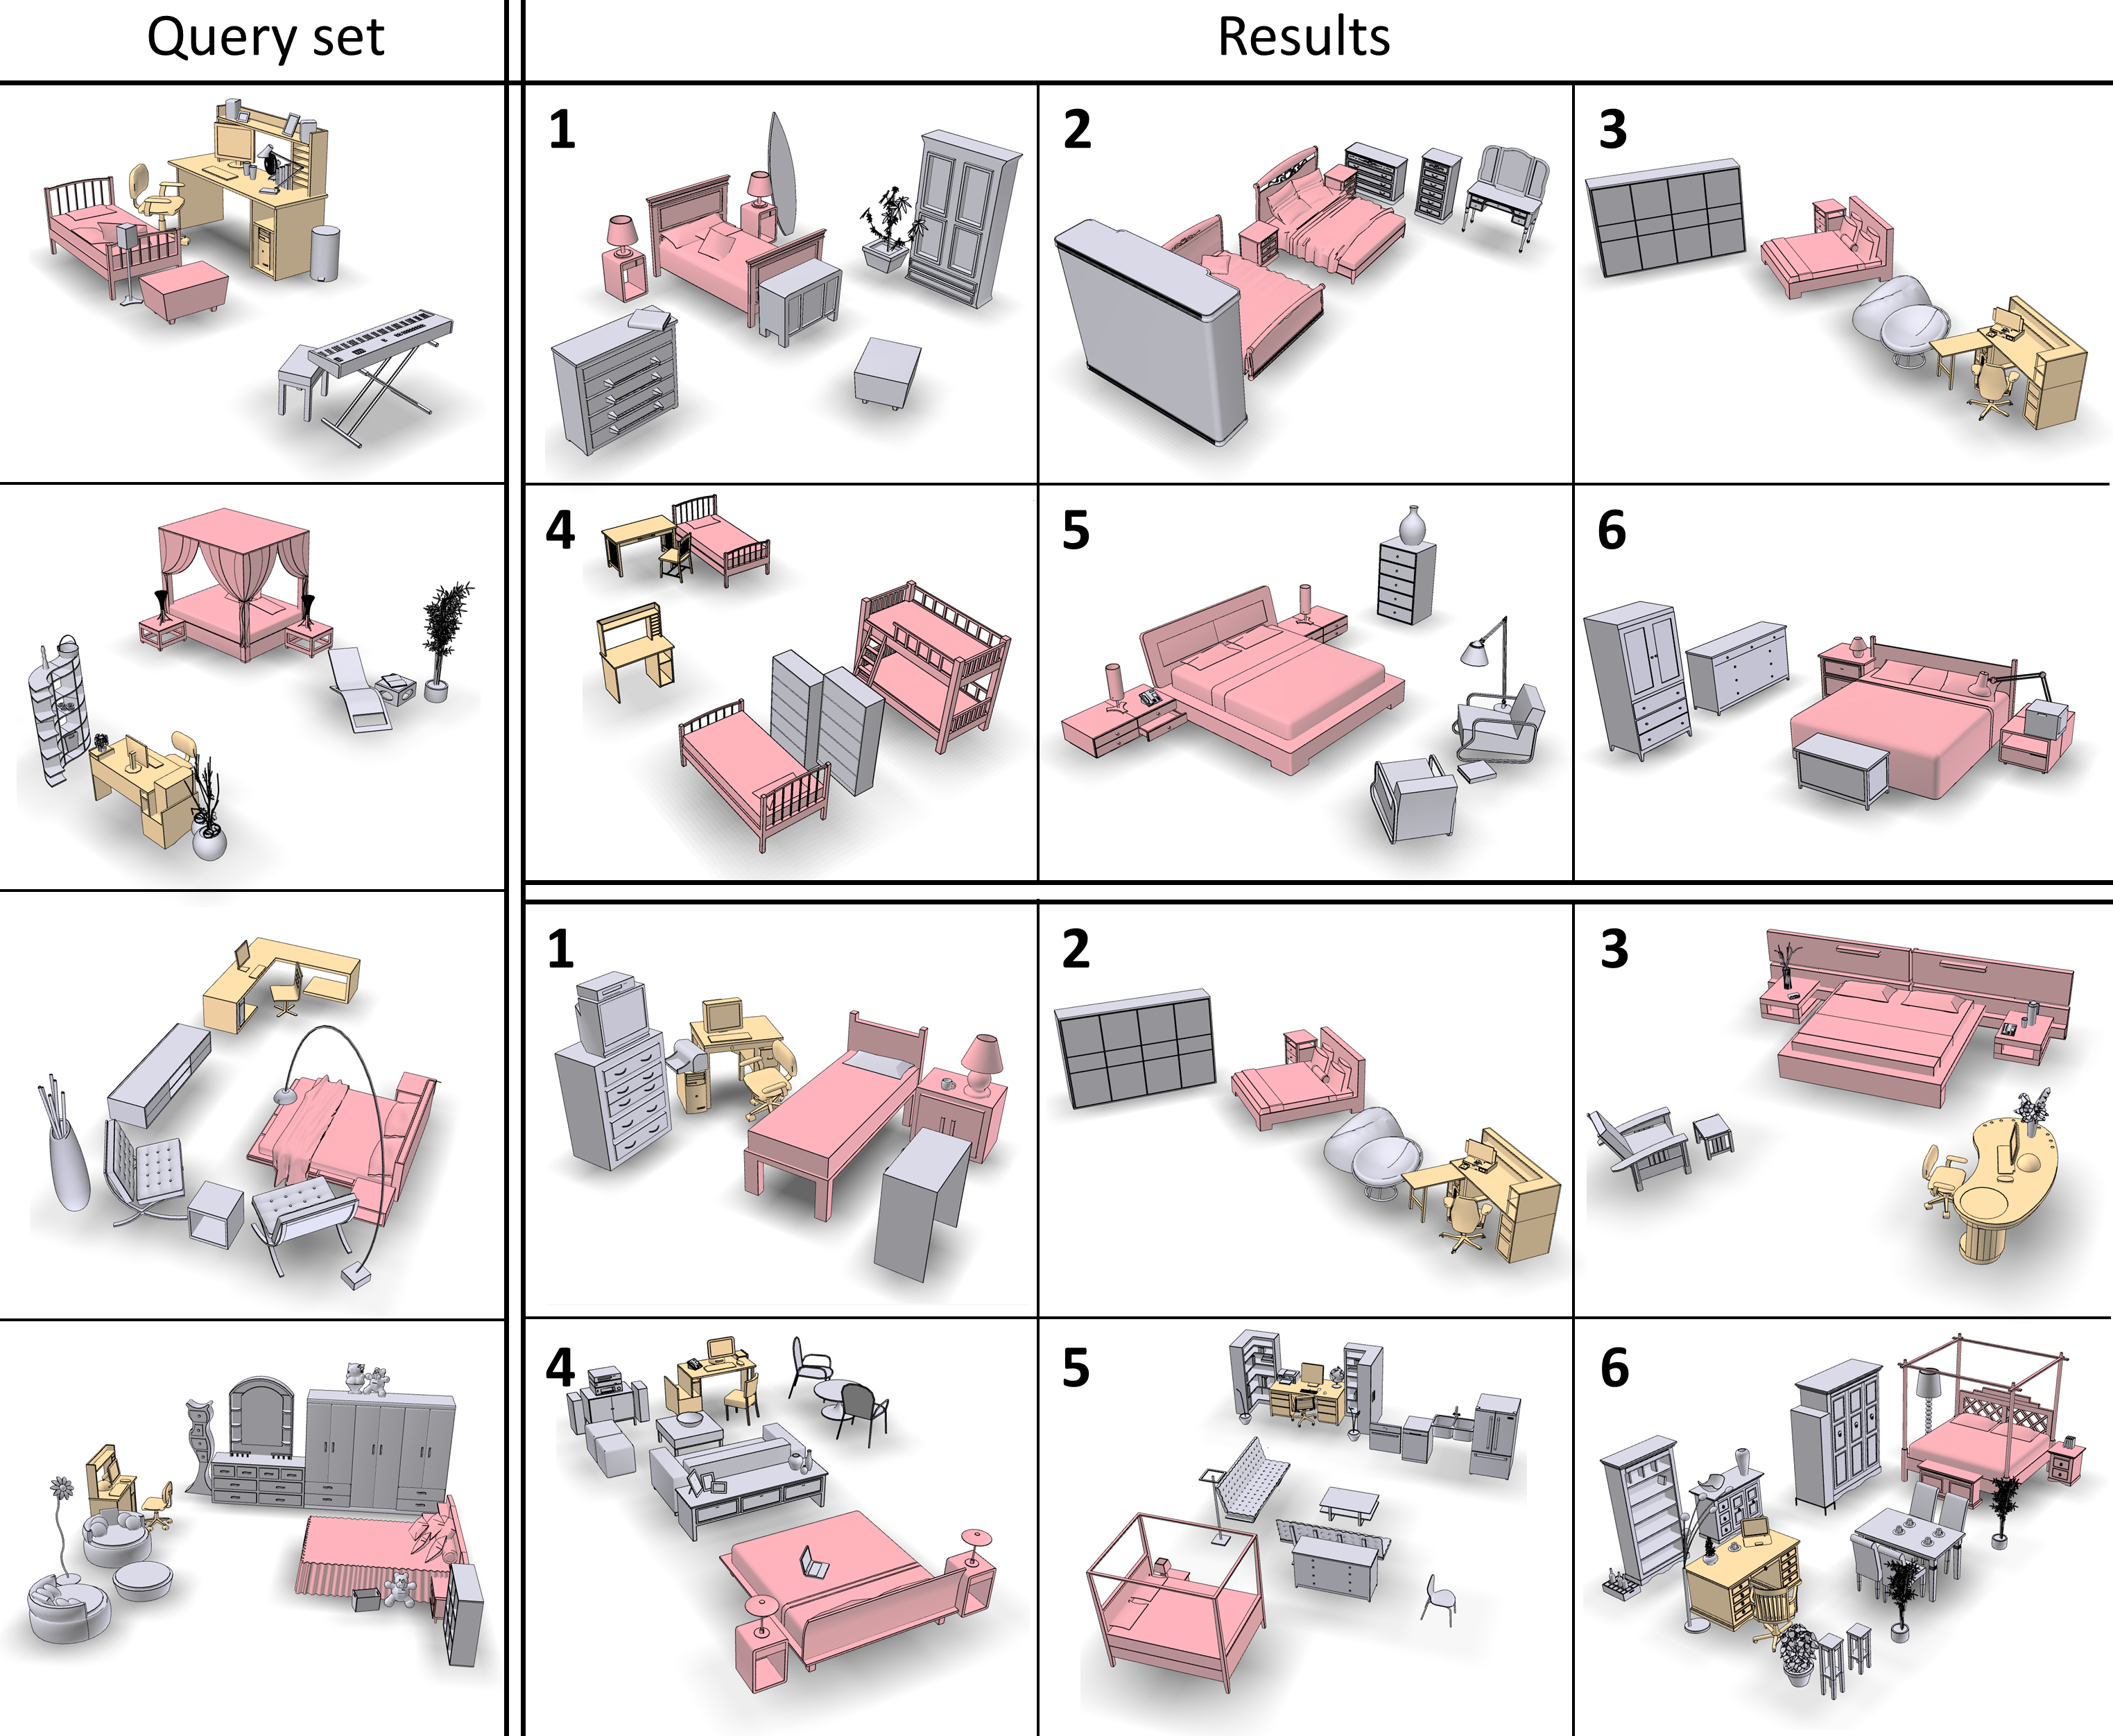
\includegraphics[width=0.98\linewidth]{fig/img/xu_sig14_multiquery}
        \vspace{-0.4cm}
    \caption{
    Multi-query retrieval takes a query set (left) and returns a ranked list of scenes (bottom-right) via focal (colored red and yellow) based scene comparison.
    Returns based on global scene similarity computed by graph kernel are also shown (top-right).
    }
    \vspace{-0.6cm}    
    \label{fig:multiquery}
\end{figure}


\paragraph*{Synthesis.}
Given an annotated scene collection, one can also synthesize new scenes that have a similar distribution of objects. The scene synthesis technique of Fisher et al.~\shortcite{Fisher:2012:CSR} learns two probabilistic models from the training dataset: (1) object occurrence, indicating which objects should be placed in the scene, and (2) layout optimization, indicating where to place the objects. Next, it takes an example scene, and then synthesizes similar scenes using the learned priors. It replaces or adds new objects using context-based retrieval techniques, and then optimizes for object placement based on learned object-to-object spatial relations.  Synthesizing example scenes might be a challenging task, thus Xu et al.~\shortcite{Xu:2013:S2S} propose modeling 3D indoor scenes from 2D sketches, by leveraging a database of 3D scenes. Their system jointly optimizes for sketch-guided co-retrieval and co-placement of all objects.


\begin{figure}[t] \centering
    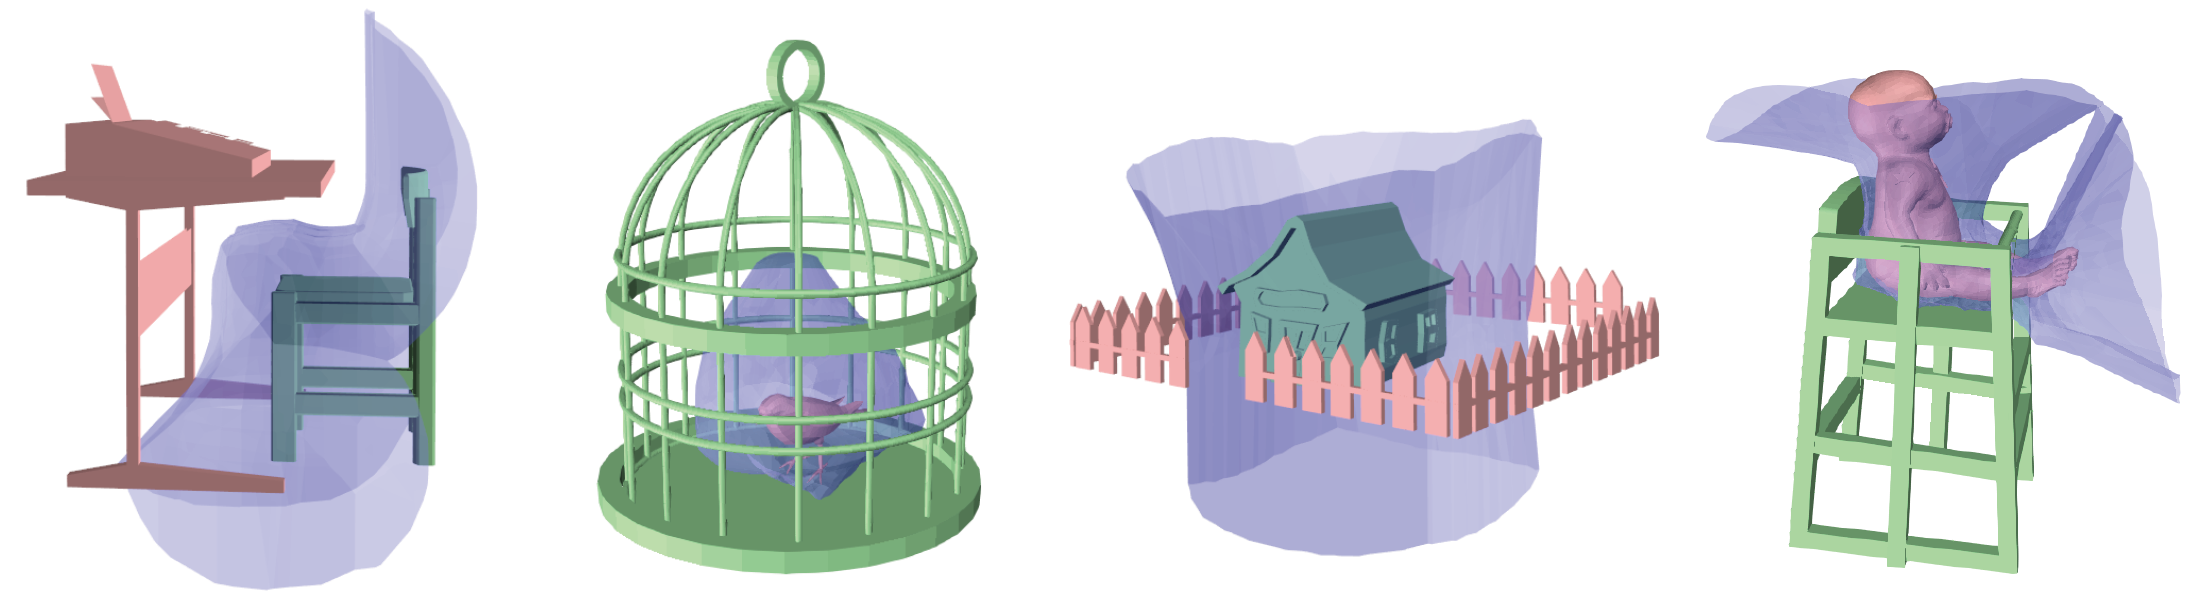
\includegraphics[width=0.99\linewidth]{fig/img/zhao_tog14_ibs}
    %\vspace{-0.2cm}
    \caption{
    The interaction bisector surface (in blue) of several two-object scenes~\cite{Zhao:2014:ISU}.
    }
    \label{fig:zhao_tog14_ibs}
\end{figure}


\paragraph*{Hierarchical scene annotation.}
All aforementioned applications take an annotated collection of 3D scenes as an input. Unfortunately, most scenes in public repositories are not annotated and thus require additional manual labeling~\cite{Fisher:2012:CSR}. Liu et al.~\shortcite{Liu:2014:CCS} address the challenge of annotating novel scenes. The key observation of their work is that understanding hierarchical structure of a scene enables efficient encoding of functional scene substructures, which significantly simplifies detecting objects and representing their relationships. Thus, they propose a supervised learning approach to estimate a hierarchical structure for novel scenes. Given a collection of scene graphs with consistent hierarchies and labels, they train a probabilistic hierarchical grammar encoding the distributions of shapes, cardinalities, and spatial relationships between objects. Such a grammar can then be used to parse new scenes: find segmentations, object labels, and hierarchical organization of objects consistent with the annotated collection (see Figure~\ref{fig:liu_siga14_sh}).

\paragraph*{Challenges and opportunities.}
The topic of 3D scene analysis is quite new and there are many open problems and research opportunities.
\emph{The first} problem is to efficiently characterize spatial relationships between objects and object groups. Most existing methods work with bounding box representation which are efficient to process, but not sufficiently informative to characterize object-to-object relationships.
For example, one cannot reliably determine the object enclosure relationship based on a bounding box.
Recently, He et al.~\shortcite{Zhao:2014:ISU} propose to use biologically-inspired bisector surface to characterize the
geometric interaction between adjacent objects and to index 3D scenes (Figure~\ref{fig:zhao_tog14_ibs}).
The bisector surface can be extended into a geometric descriptor for contextual modeling of the functionality of a 3D object in a given scene~\cite{hu:icon:2015}.
%
\emph{Second}, most existing techniques heavily rely on expert user supervision for scene understanding. Unfortunately, online repositories rarely have models with reliable object tags. Therefore there is a need for methods that can leverage scenes containing only partial and/or noisy annotations.
%most analysis rely on the availability of object labels, given the fact that the structural layout
%of scenes is mostly loose and spatial relationship is not always easy to be characterized geometrically.
%This is quite restrictive since most scene models from the web do not possess reliable object tag.
%Therefore, finding more powerful feature to characterize scenes and achieving tag-free analysis become indispensable.
%
\emph{Finally}, the popularity of commodity RGBD cameras has significantly simplified the acquisition of indoor scenes. This emerging scanning technique opens space for new applications such as online scene analysis~\cite{Zhang:2014:OSA,Xu:2015:ACS}.  %The availability of image data that come with RGBD scans also enables the enhancement of geometric representations with appearance information.

%On the other hand, the calibrated image and depth data help to relate 3D scenes with images, enabling bidirectional transfer of information such as labels, texture, etc.




\section{Exploration and organization}
\label{sec:exploration}
\rev{The rapidly growing quantity and variety of digital 3D models in large online collections have caused an emerging need to develop algorithms and techniques that effectively organize these large collections and allow users to interactively explore them.
% provide rich content that can be directly used in many applications.  For example, an architect can furnish a digital building using models from a repository.
For example, an architect might furnish a digital building by searching through databases organized according to furniture types, regions of interest and design styles.  Likewise, an industrial designer can explore shape variations among existing products when creating a new object.
%Large repositories of 3D models provide opportunities in many domains, but also necessitate developing effective tools for organizing model collections.
Most existing repositories only support text-based search, relying on user-entered tags and titles. This approach suffers from inaccurate and ambiguous tags, often entered in different languages. \rev{While it is possible to try using shape analysis to infer consistent tags as discussed in Section \ref{sec:classification}, it is difficult to convey stylistic and geometric variations using only text.} An alternative approach can be to perform shape, sketch, or image based queries. However, to formulate such search queries the user needs to have a clear mental model of the shape that should be retrieved.
Thus, some researchers focus on providing tools for \emph{exploring} shape collections. Unlike search, exploration techniques do not assume a-priori knowledge of the repository content, and help the user to understand geometric, topological, and semantic variations within the collection.}

%With the learned variations and mutual relations between different shapes,
%some works studied the organization of shape collections through grouping and relating the shapes in a systematic way.
%Combing with effective visualization, such organization can provide a global view of the entire database~\cite{Huang:2013:QOC}.

\paragraph*{Problem statement and method categorization.}
Data exploration and organization is a classical problem in data analysis and visualization~\cite{Paulovich:2011:PLP}. Given a data collection, the research focuses on \emph{grouping and relating data points, learning the data variations in the collection, and organizing the collection into a structured form},
to facilitate retrieval, browsing, summarization, and visualization of the data, based on efficient \emph{interfaces or metaphors}.

The first step to organizing model collections is to devise appropriate metrics to relate different data points. Various similarity metrics have been proposed in the past to relate entire shapes as well as local regions on shapes. In particular, previous sections of this document cover algorithms for computing global shape similarities (Section \ref{sec:classification}), part-wise correspondences (Section \ref{sec:segmentation}), and point-wise correspondences (Section \ref{sec:matching}). In this section, we will focus on techniques that take advantage of these correlations to provide different interfaces for exploring and understanding geometric variability in collections of 3D shapes.
We categorize the existing exploration approaches based on four aspects:
\begin{itemize}
\item \textbf{Metaphor:} a user interface for exploring shape variations. We will discuss five basic exploration interfaces, ones that use proxy shapes (templates), regions of interest, probability plots, query shapes, or continuous attributes.
\item \textbf{Shape comparison:} techniques used to relate different shapes. We will discuss techniques that use global shape similarities, as well as part or point correspondences.
\item \textbf{Variability:} shape variations captured by the system. Most methods we will discuss rely on geometric variability of shapes or parts. Some techniques also take advantage of topological variability; that is, variance in number of parts or how they are connected (or variance in numbers of objects and their arrangements in scenes).
\item \textbf{Organizational form:} a method to group shapes. We will discuss methods that group similar shapes to facilitate exploring intra-group similarities and inter-group variations, typically including clustering and hierarchical clustering.
\end{itemize}
Table~\ref{tab:exploration} summarizes several representative works in terms of these  aspects.
\rev{In the remaining part of this section we list several recent techniques which are grouped based on the exploration metaphor.}

\begin{table}[!t]
\centering
\begin{tabular}{l|c|c|c|c} \hline
                         Method                & Meta. & Comp. & Var.    & Org.
 \\ \hline\hline
             \cite{Ovsjanikov:2011:ECV} & temp. & simi. & geom.  & n/a
 \\ \hline   \cite{Kim:2013:lpt}         & temp. & part & both    & cluster
 \\ \hline   \cite{Averkiou:2014:spm}  	   & plot & part & both   & cluster
 \\ \hline   \cite{Kim:2012:FC}         & ROI & point & both      & n/a
 \\ \hline   \cite{Rustamov:2013:SD}  & ROI   & point & geom.     & n/a
 \\ \hline   \cite{Huang:2014:FMN}       & ROI & point & both      & cluster
 \\ \hline   \cite{Xu:2014:OHSC}         & ROI & simi. & topo.     & cluster
 \\ \hline   \cite{Fish:2014:MR}         & plot & part  & geom.     & cluster
 \\ \hline   \cite{Huang:2013:QOC}       & query & simi. & both   & hierarchy
 \\ \hline
\end{tabular}
\caption{\rev{A summary of several recent works over four aspects.
         \underline{Meta}phor: \underline{temp}lates, surface painted \underline{ROI}s,
         probability distribution \underline{plot}s, or \underline{query} shapes.
         Shape \underline{Comp}arison: shape \underline{simi}larity, \underline{part} or \underline{point} correspondence.
         \underline{Var}iability: \underline{geom}etry, \underline{topo}logy or \underline{both}.
         \underline{Org}anization Form: \underline{cluster} or \underline{hierarchy}.
         %For scene exploration, topology refers to structural graphs about scene layout~\cite{Xu:2014:OHSC}.
         }}
\label{tab:exploration}
\end{table}


\paragraph*{Template-based exploration.}
Component-wise variability in position and scale of parts reveals useful information about a model collection. Several techniques use box-like templates to show variations among models of the same class. Ovsjanikov et al.~\cite{Ovsjanikov:2011:ECV} describe a technique for learning these part-wise variations without solving the challenging problem of consistent segmentation. First, they use the segmentation of a single shape to construct the initial template. This is the only step that needs to be verified and potentially fixed by the user. The next goal is to automatically infer deformations of the template that would capture the most important geometric variations of other models in the collection.  They hypothesize that all shapes can be projected on a low-dimensional manifold based on their global shape descriptors. Finally, they reveal the manifold structure by deforming a template to fit to the sample points. Directions for interesting variations are depicted by arrows on the template and the shapes that correspond to the current template configuration are presented to the user.% \vova{perhaps we should have a figure here}.

The descriptor-based approach described above assumes that all intra-class shapes share the same parts and that there exists a low-dimensional manifold that can be captured by deforming a single template. These assumptions do not hold for large and diverse collections of 3D models.  To tackle this challenge, Kim et al.~\cite{Kim:2013:lpt} proposed an algorithm for learning several part-based templates capturing multi-modal variability in collections of shapes. They start with an initial template that includes a super-set of all parts that might occur in a dataset, and jointly learn part segmentations, point-to-point surface correspondence as well as a compact deformation model. The output is \emph{a set of templates} that groups the input models into clusters, capturing their styles and variations.

\paragraph*{ROI-based exploration.}
Not all interesting variations occur at the scale of parts: they can occur at sub-part scale, or span multiple sub-regions from multiple parts. In these cases the user may prefer to select an arbitrary region on a 3D model and look for more models sharing similar regions of interest. Such detailed and flexible queries require a finer understanding of correspondences between different shapes. Kim et al.~\cite{Kim:2012:FC} propose fuzzy point correspondences to encode the inherent ambiguity in relating diverse shapes. Fuzzy point correspondences are represented by real values specified for all pairs of points, indicating how well the points correspond.  They leverage transitivity in correspondence relationships to compute this representation from a sparse set of pairwise point correspondences.  The interface proposed by Kim et al. allows users to paint regions of interest directly on a surface and then retrieve similar regions among other shapes, or even show geometric variations found in the selected region (see Figure~\ref{fig:kim_sig12_fc}).
\begin{figure}[t]
\centering
    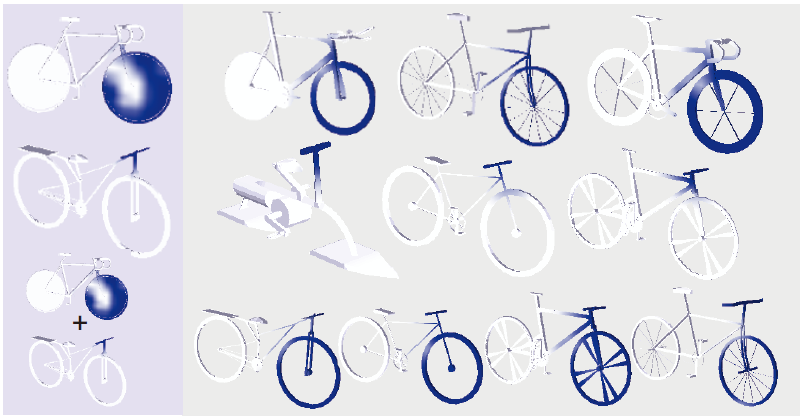
\includegraphics[width=1.0\columnwidth]{fig/img/kim_sig12_fc}
    %\vspace{-0.4cm}
    \caption{Shape exploration based on fuzzy correspondence. The user paints a region of interest (ROI) on a query shape (left column), and the method
    sorts models based on their similarity within the region (right).}
    \label{fig:kim_sig12_fc}
\end{figure}



One limitation of correspondence-based techniques is that they typically do not consider the entire collection when estimating shape differences.  Rustamov et al.~\cite{Rustamov:2013:SD} focus on a fundamental intrinsic representation for shape differences.  Starting with a functional map between two shapes, that is, a map that describes a change of functional basis, they derive a shape difference operator revealing detailed information about the location, type, and magnitude of distortions induced by a map. This makes shape difference a quantifiable object that can be co-analyzed within a context of the entire collection. They show that this deeper understanding of shape differences can help in exploration. For example, one can embed shapes in a low-dimensional space based on shape differences, or use shape difference to interpolate variations by showing ``intermediate" shapes between two regions of interest.
%
To extend these technique to man-made objects, Huang et al.~\cite{Huang:2014:FMN} construct a consistent functional basis for shape collections exhibiting large geometric and topological variability. They show that the resulting consistent maps are capable of capturing discrete topological variability, such as variance in the number of bars of the back of a chair.

\paragraph*{ROI-based scene exploration.}
Recent works on organizing and exploring 3D visual data mostly focus on object collections. Exploring 3D scenes poses additional challenges since scenes typically exhibit more structural variations. Unlike man-made objects that usually contain a handful of object parts, scenes can contain anywhere from ten to hundreds of objects.  Not only this, but the objects themselves do not typically have a prescribed rigid arrangement with respect to each other. Thus, global scene similarity metrics, such as the graph kernel based one used in \cite{Fisher:2012:CSR} are limited to organizing datasets based on very high-level features, such as scene type.
%
Xu et al.~\cite{Xu:2014:OHSC} advocate that 3D scenes should be compared from the \emph{perspective} of a particular focal point which is a representative substructure of a specific scene category. Focal points are detected through contextual analysis of a collection of scenes, resulting in a clustering
of the scene collection where each cluster is characterized by its representative focal points (see Section~\ref{sec:scene}).
%
Consequently, the focal points extracted from a scene collection can be used to organize collection into an interlinked and well-connected cluster
formation, which facilitates scene exploration. Figure~\ref{fig:xu_sig14_expl} shows an illustration of such cluster-based organization
and an exploratory path transiting between two scene clusters/categories.


%\teaser{
\begin{figure}[t]
\centering
    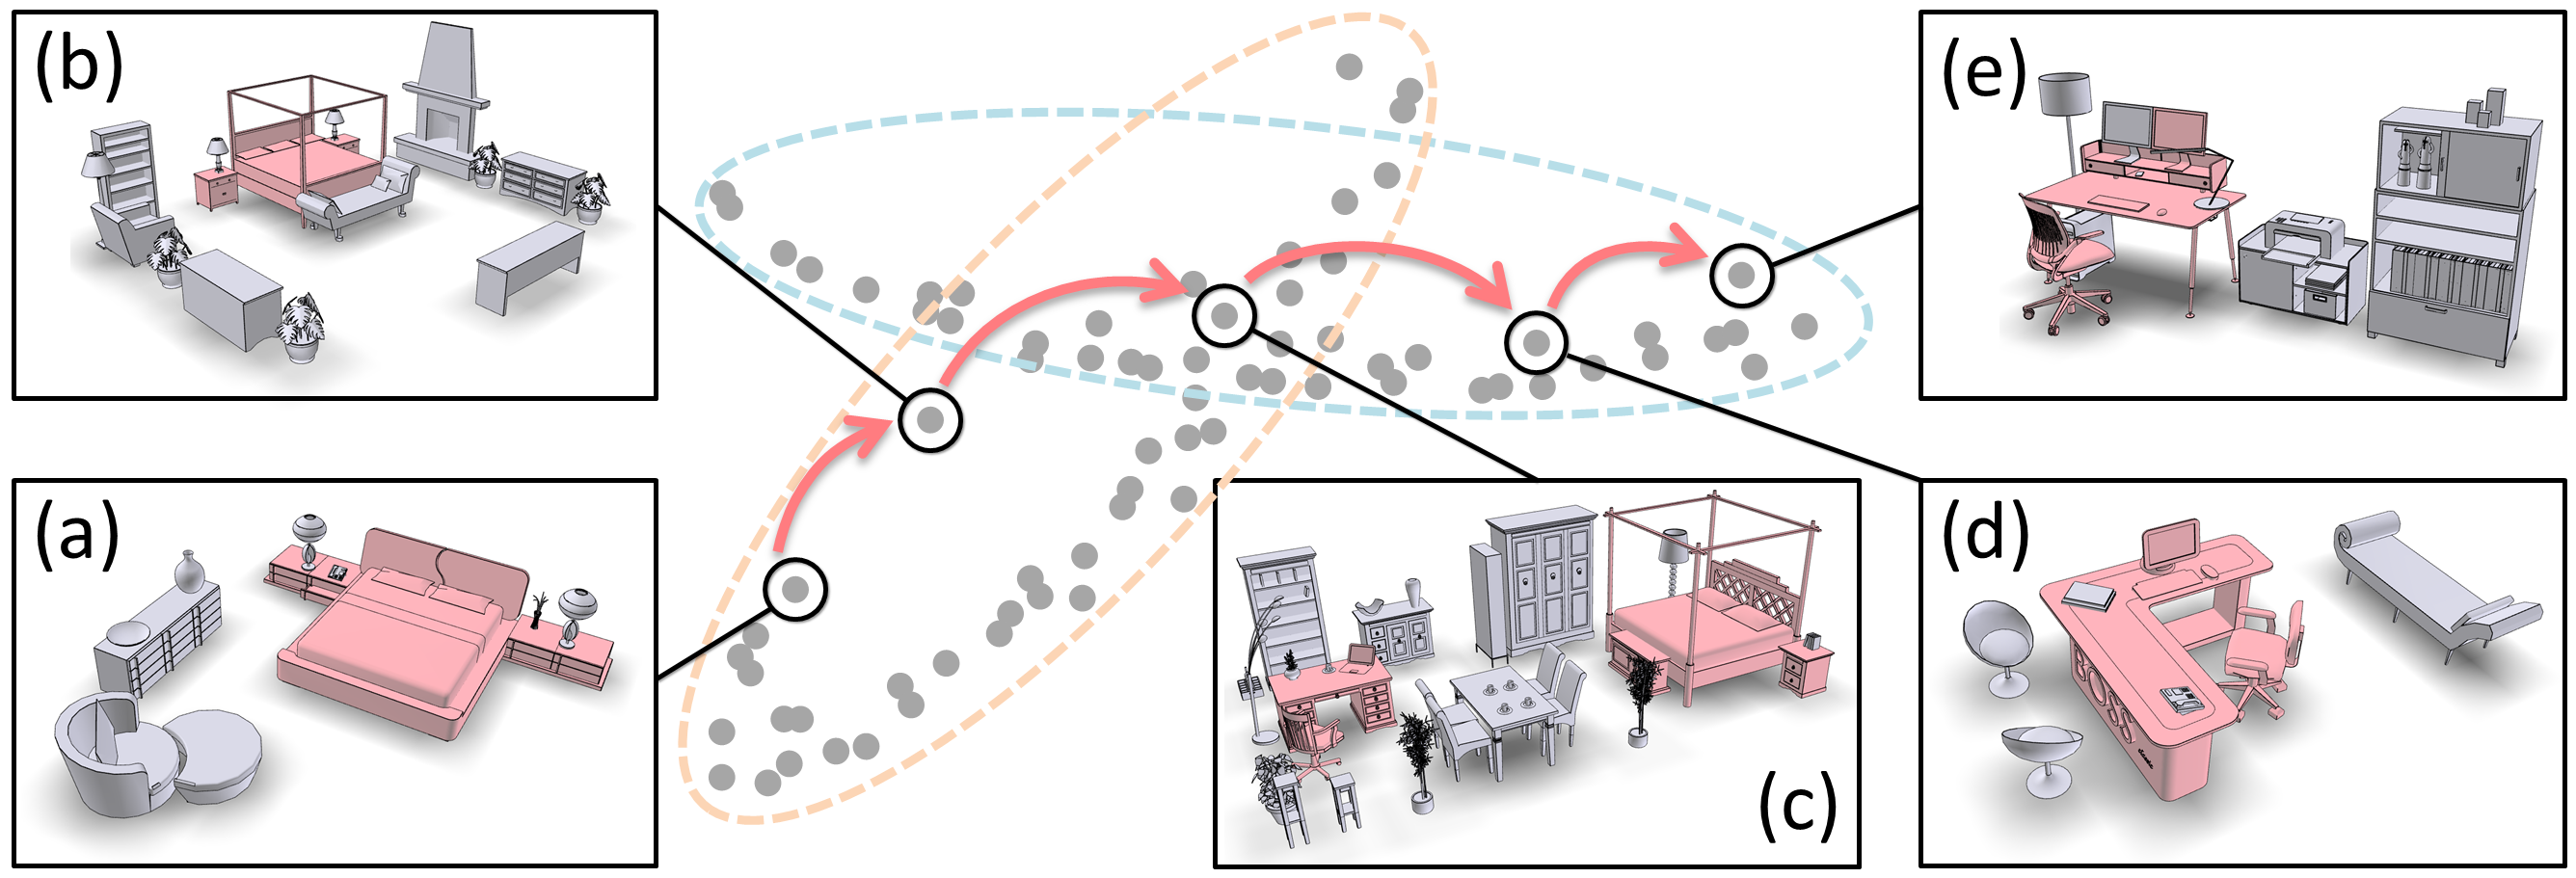
\includegraphics[width=0.99\linewidth]{fig/img/xu_sig14_expl}
%    \vspace{-0.4cm}
    \caption{
    Focal-based scene clustering produces overlapping clusters, which is due to hybrid scenes possessing multiple focal points.
    An exploratory path, from (a) to (e), through the overlap, smoothly transit between the two scene clusters,
    representing bedroom and offices, respectively.}
    \label{fig:xu_sig14_expl}
\end{figure}
%}


\paragraph*{Plot-based exploration.}
All aforementioned exploration techniques typically do not visualize the probabilistic nature of shape variations.  Fish et al.~\cite{Fish:2014:MR} study the configurations of shape parts from a probabilistic perspective, trying to indicate which shape variations are more likely to occur.  To learn the distributions of part arrangements, all shapes in the family are pre-segmented consistently.
The resulting set of probability density functions (PDFs) characterizes the variability of relations and arrangements across different parts. A peak in a PDF curve represents that particular a configuration of the related parts frequently appeared among several shapes in the family. The multiple PDFs can be used as interfaces to interactively explore the shape family from various perspectives.
Averkiou et al.~\cite{Averkiou:2014:spm} use part structure inferred by this method to produce a low-dimensional part-aware embedding of all models. The user can explore interesting variations in part arrangements simply by moving the mouse over the 2D embedding. In addition, their technique allows the synthesis of novel shapes by clicking on empty spaces in the embedded space.  Upon clicking, the system would deform parts from neighboring shapes to synthesize a novel part arrangement.

\begin{figure}[t]
\centering
    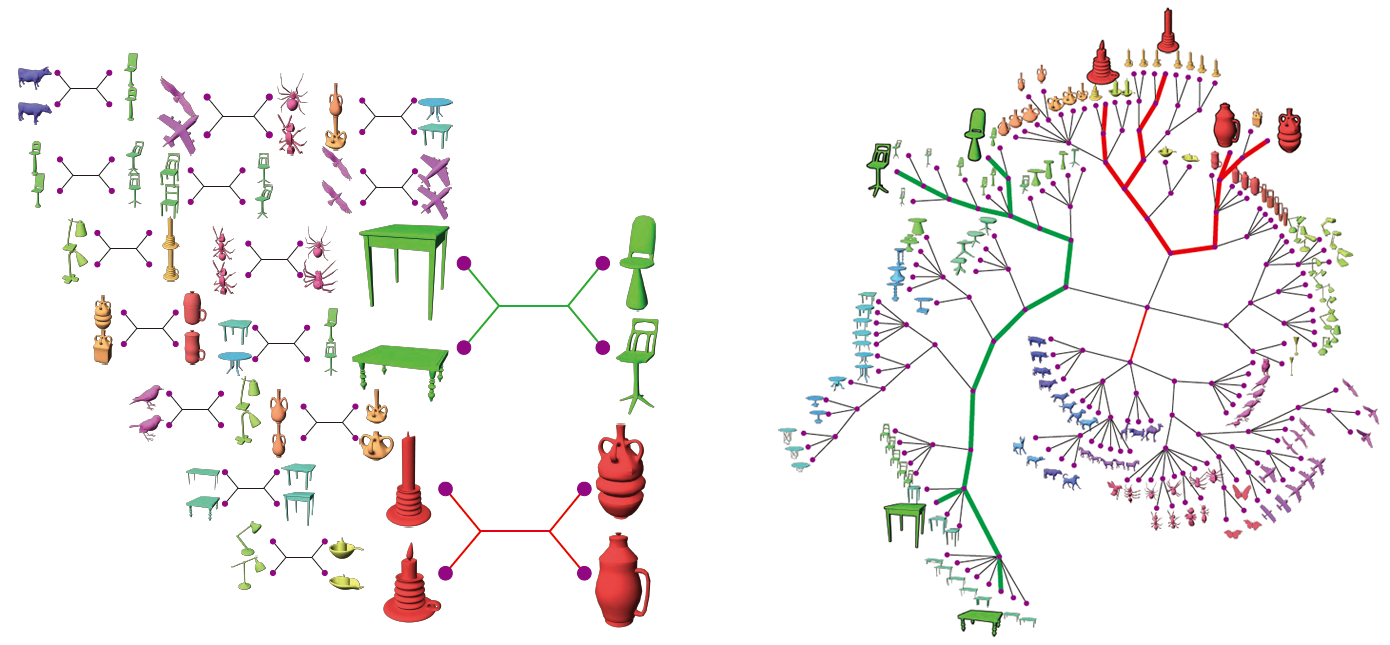
\includegraphics[width=1.0\columnwidth]{fig/img/huang_sig12_quartet}
    %\vspace{-0.4cm}
    \caption{Given a set of heterogeneous shapes, a reliable qualitative similarity is derived from quartets composed of two pairs of objects (left).
    Aggregating such qualitative information from many quartets computed across the whole set leads to a categorization tree as a hierarchical
    organization of the input shape collection (right).}
    \label{fig:huang_sig12_quartet}
\end{figure}



\paragraph*{Query-based exploration.}
For a heterogeneous shape collection encompassing diverse object classes, it is typically not possible to characterize part-structure and correspondences between all pairs of shapes. Even global shape similarity is not a very reliable feature in this setting, which makes organizing and exploring heterogeneous collections especially difficult.
To address this challenge, Huang et al.~\cite{Huang:2013:QOC} introduce qualitative analysis techniques from the field of bioinformatics. Instead of relying on quantitative distances, which may be ill-applied between dissimilar shapes, the method considers a more reliable \emph{qualitative similarity} derived from \emph{quartets} composed of two pairs of objects. The shapes that are paired in the quartet are close to each other and far from the shapes in the other pair, where distances are estimated from multiple shape descriptors.  They aggregate this topological information from many quartets computed across the entire shape collection, and construct a hierarchical \emph{categorization tree} (see Figure~\ref{fig:huang_sig12_quartet}). Analogous to the phylogenetic trees of species, this categorization tree of a shape collection provides an overview of the shapes as well as their mutual distance and hierarchical relations. Based on such an organization, they also define the degree of separation chart for every shape in the collection and apply it for interactive shape exploration.

\paragraph*{Attribute-based exploration.}
Yet another approach seeks to allow users to interactively explore shapes with continuously valued semantic attributes.  Blanz and Vetter \cite{Blanz:1999:MMS} provide an interface to explore faces based on continuous facial attributes, such as ``smile'' or ``frown'', \rev{built upon the face parametric model (Section \ref{sec:recon}}). Similarly, Allen et al.~\cite{Allen:2003:SHB} allow users to explore the range of human bodies with features such as height, weight, and age. Chaudhuri et al.'s~\cite{Chaudhuri:2013:ACC} interface enables exploration of shape parts according to learned strengths of semantic attributes (Figure \ref{fig:attribit}). 



\section{Discussion}
\label{sec:conclusion}
There is no ``magic recipe'' for developing new data-driven and machine learning
applications in geometry processing and computer graphics. Yet, there are some important considerations one needs to make in devising a data-driven method, including computational complexity, scalability, applicability issues, proper
evaluation procedures and
limitations. In this section, we briefly discuss these issues.%\fix


\paragraph*{Computational complexity.}
As explained in Section \ref{sec:overview}, data-driven shape analysis and processing algorithms generally contain several stages (Figure \ref{fig:overview}). The complexity of each stage varies and largely depends on the number of input shapes, resolution of the input shape representation (number of faces, surface points, pixels or voxels), as well as the number and type of the used geometric features. The feature extraction stage is usually executed per each shape, thus, its time complexity often tends to be linear in the number of input shapes. Local geometric features, such as surface curvature or PCA-based descriptors, are usually computed within a small neighborhood around each vertex, face, or surface point, thus their extraction depends linearly on the number of these primitives in the input shape representation. Extracting geometric features that capture less local or global information about the shape, such as shape diameter, geodesic distance-based features or heat-kernel descriptors, is often computationally more intensive i.e., super-linear in the number of primitives.
%For example, computing exact geodesic distances over a mesh with Mitchell et al.'s algorithm \cite{Mitchell:1987:DGP} has worst case O($K^2 \log K$) time complexity, where $K$ is the number of mesh edges.

During the learning and inference steps, data-driven methods usually solve an optimization problem, which involves minimizing or maximizing a function e.g., a data likelihood function. In general, optimization techniques inhabit a wide range of computational complexities. For example, if the optimization involves the least-squares solution of a linear system, as in the case of linear regression, the complexity is O($N \cdot F^2$), where $N$ is the number of input training examples and $F$ is the dimensionality of the input feature vector. If optimization is performed through a steepest descent algorithm, the complexity is $O(N \cdot F)$ per parameter update step. However, the performance of iterative optimization algorithms depends on the number of steps, which in turn varies according to their convergence properties and the function they optimize. We refer the reader to \cite{Nocedal:2006:NO,Koller:2009:PGM,Solomon:2015:NA} for an in-depth discussion on the computational complexity and convergence properties of various optimization and inference algorithms.



\paragraph*{Scalability.}
Data-driven methods are inherently bound up with the input data.
Rapid developments in capturing and modeling techniques have engendered the growth of
3D shape and scene repositories over recent years, which  have  in turn influenced the advancement of data-driven geometry processing.
This is evidenced by the fact that the number of training shapes employed in data-driven geometry
processing  techniques has grown from a few tens~\cite{Kalogerakis:2010:LMS,Sidi:2011:CS}
to several thousands~\cite{Kim:2013:lpt,Huang:2014:FMN}. On the one hand, the increasing
availability of 3D data can improve the accuracy and generalization of data-driven
methods. On the other hand, issues of scalability arise. More data causes
longer processing times, which in turn makes the debugging of such methods harder for developers. The scalability issues are further
exacerbated by the complexity (i.e., high-dimensionality) of the 3D geometric feature representations. Potential workarounds include debugging
the pipeline of these methods on smaller datasets before turning to larger ones,  trying simpler learning techniques before switching to more complex ones, or making use of computing clusters for executing offline steps.%\fix

\paragraph*{Scope of application.}
Not every problem in shape analysis and processing is well suited to be solved by a data-driven method. When the underlying rules, principles, and parameters can be manually and unambiguously specified in a problem, then non-data-driven  methods should be considered for it.
For example, deforming a shape with an elastic material and known physical parameters
and forces  can be addressed by a physics-based method rather than a data-driven one. In contrast, there are several problems in shape analysis and processing for
which it is hard, or even impossible, to hand-design a set of rules and principles, or quantify them through manually specified parameters. This is often the case for
problems that involve shape and scene recognition, high-level processing, structure parsing, co-analysis, reconstruction from noisy missing data, and modeling with high-level user input. Shape co-analysis (e.g., co-segmentation), in particular, requires
estimating several possible geometric and semantic correlations among input shapes, which would be practically impossible to capture through hand-designed rules. Data-driven methods that automatically compute geometric, semantic and structural relationships in the input shapes are
more appropriate for such co-analysis problems~\cite{Xu:2010:SCS,Huang:2011:JSS,Huang:2013:SDP}.
Another example can be found in the problem of shape style analysis. Although humans have an
innate sense of style similarity, it is hard to manually quantify geometric criteria
for modeling the stylistic similarity of shapes. A style analysis algorithm whose parameters are learned through a data-driven method is much more well-suited to perform this quantification~\cite{liu:style:2015,lun:style:2015}.



\paragraph*{Evaluation.}
Correctly evaluating the predictive performance of data-driven methods should be another important consideration for researchers of such methods. A common pitfall is to evaluate the predictive performance of a data-driven method
with the same dataset on which it was trained on (e.g., through supervised learning), or a dataset for
which any parameters of the method were manually tuned. The risk here is that the method
might not be able to generalize to any other datasets beyond the ones used in training
or hand-tuning. A method that simply memorizes
the training dataset, or overfits a model to a particular dataset, will obviously perform well there. However, if its performance on other datasets is poor, the method is effectively useless. The best practice is to introduce training and test splits of the input datasets. The models and parameters should then be learned or tuned exclusively on the training portion, and evaluated exclusively on the testing portion. To insure fair-play, it is also necessary that different data-driven methods be compared using the same training and test splits.%\fix



\paragraph*{Limitations.}
\fix{
The data-driven approach to shape analysis and processing is bound by a few
limitations that we summarize below. We also discuss potential workarounds to overcome some of these.
 \begin{itemize}
\item {\bf Generalization guarantees.} It is generally hard to provide any guarantees about the generalization performance of data-driven algorithms. In other words, when a data-driven algorithm makes use of a particular dataset for training, it is often impossible to predict how well it will generalize to other datasets beforehand. Although statistical error bounds can be provided under particular assumptions on data distributions, in particular within the context of the Probably Approximately Correct learning theory  \cite{Valiant:1984:TL} or the Bayes decision theory
\cite{Fukunaga:1990:ISP}, these assumptions often cannot be validated in practice.
\vspace{6pt}
\item {\bf Complexity and scalability.} As discussed above, data-driven methods are
computationally intensive in general. The complexity of data-driven methods depends on the number of input training shapes. As a general rule of thumb, the accuracy of data-driven methods improves with more training data.  On the other hand, this comes at a higher computational cost during training time.
\vspace{6pt}
\item {\bf Size of 3D shape datasets.} Despite their recent growth, the size of
available 3D shape datasets remains much smaller than those used in computer
vision and natural language processing (e.g., image and text datasets). As a result, overfitting remains
a common issue with data-driven methods for 3D shape processing.
Overfitting occurs when a learned model,
or function, captures random error, noise, or patterns specific only to the input training dataset instead of the underlying, correct relationships in the data. It usually occurs when the learned model, or function, is excessively complex, e.g., having an extremely large number of parameters relative to the size of the training dataset. To mitigate this issue, regularization techniques can be used to favor simpler
models and functions \cite{Ng:2004:FSL,DOMINGOS:2012:ML}. Another promising approach is to use both 3D shapes and 2D images as input
to data-driven methods, or in other words, to perform co-analysis of image and shape
data. We discuss this issue as one important future research direction for further
development in data-driven methods in the next section.
\vspace{6pt}
\item {\bf Data collection.} Data-driven techniques rely on the availability of data for the particular problem they attempt to solve. Gathering training data for several geometry processing tasks is often not an easy task, especially when human labor is involved to process or annotate geometric data.  Although crowdsourcing Internet marketplaces, such as Amazon Mechanical Turk~\cite{amt09}, can help gather training data efficiently, online questionnaires and user studies still require careful design, monetary compensation, and participant consistency checks.
    \vspace{6pt}
\item {\bf From data to knowledge.}
    Data-driven methods put particular emphasis on discovering patterns and models that explain the input data and provide useful insights to the problem being
solved. However, these learned patterns and models might not always be readily interpretable  i.e., might not correspond to ``easy-to-understand'' rules. This
 is a common situation when one treats the internals of the data-driven method (e.g.,
the learning process) as a ``black box'' without first  trying to understand their exact
functionality in detail. In general, interpreting such patterns and models requires significant time and effort.
\end{itemize}
}%\fix








\section{Conclusion and open problems}
\label{sec:conclusion}

In this survey, we have so far discussed state-of-the-art on data-driven methods for 3D shape analysis and processing. We also presented the main concepts and methodologies used to develop such methods. We hope that this survey will act as a tutorial that will help researchers develop new data-driven algorithms related to shape analysis and processing. There are several exciting research directions that have not been sufficiently explored so far in our community that we discuss below:

\paragraph*{Joint analysis of 2D and 3D data.}
Generating 3D content from images requires building mappings from 2D to 3D space. Unfortunately, the problem remains largely ill-posed.  However, with the help vast quantities of 2D images available on the web, effective priors can be developed to map 2D visual elements or features to 3D shape and scene representations.
Indeed, we have in fact seen recent attempts made in this very vein of thought with some success in ~\cite{Su:2014:EID,Aubry14,Li:2015:JE,Hueting:2015:CL,Su:2015:RfC}, which attempts depth estimation through joint analysis over 2D image collections and 3D model databases.  We have also seen success of the joint analysis framework in the setting of texture-data with \cite{Yumer:CST:2014}, which attempts cosegementation of textured 3D shapes.


%Another possibility is to investigate the inverse procedure: by building connections from 3D shapes to 2D images for shape understanding. The work of image-driven shape segmentation by Wang et al. \cite{Wang:2013:PAS} is one such example. % \vangelis{moved it to the main text}
Following this line, it would be interesting to jointly analyze and process multi-modal visual data, including depth scans and videos. The key challenge lies in the integration of heterogeneous information in a unified learning framework.

\paragraph*{Better and scalable shape analysis techniques.} Many data-driven applications rely on high-quality shape analysis results, particularly shape segmentations and correspondences. We believe it is important to further advance research in both these directions. This includes designing shape analysis techniques for specific data and/or making them scalable to very large datasets, especially recently emerging large-scale richly-annotated repositories~\cite{Shapenet}.

\paragraph*{From geometry to semantics and vice versa.}
Several data-driven methods have tried to map 2D and 3D geometric data to high-level concepts, such as shape categories, semantic attributes, or part labels.
Gathering relevant training data is a key component in achieving this aim, a task which remains a non-trivial endeavor.  Several recent promising works employ crowdsourcing to address this issue~\cite{Chen:2009:BMS,Chaudhuri:2013:ACC,lun:style:2015,liu:style:2015,Yumer:2015:SSE}.  Existing methods deal with cases where only a handful of different entities are predicted for input shapes or scenes.
Scaling these methods to handle thousands of categories, part labels and other such entities, as well as attaining human-level performance, is an open problem.
The opposite direction is also interesting and insufficiently explored: generating shapes and scenes based on high-level specifications such as shape styles, attributes, or even natural language.  Such approaches may even potentially be combined with further diverse inputs, such as sketches and interactive handles, in the shape-generating pipeline. WordsEye \cite{Coyne:2001:WAT} was an early attempt to bridge this gap, yet requires extensive manual mappings.

\paragraph*{Understanding function from geometry.}
The geometry of a shape is strongly related to its functionality, including the shape's relationship to human activity. Thus, analyzing shapes and scenes requires some understanding of their function. The recent works by Laga et al.~\cite{Laga:2013:GCS}, Kim et al.~\cite{Kim14} and Hu et al.~\cite{hu:icon:2015,hu:icon2:2016} are important
examples of data-driven approaches that take into account functional aspects of shapes in the process of their analysis.
In addition, data-driven methods can guide the synthesis of shapes that can be manufactured or 3D printed based on given functional specifications; an example of such an attempt is reflected in the work of Schulz et al \cite{Schulz:2014:DFE}.


\paragraph*{Data-driven shape abstractions.}
It is relatively easy for humans to communicate the essence of shapes with a few lines, sketches, and abstract forms. Developing methods that can build such abstractions automatically has significant applications in shape and scene visualization, artistic rendering, and shape analysis. There are a few data-driven approaches to line drawing \cite{Cole:2008:WDP,Kalogerakis:2009:DDC,Kalogerakis:2012:LHP}, saliency analysis \cite{Chen:2012:SPO}, surface abstraction \cite{Yumer:2012:CSC}, and viewpoint preferences \cite{Secord:2011:PMO} related to this goal. Matching human performance in these tasks is still a largely open problem, while synthesizing and editing shapes using shape abstractions as input remains a significant challenge.

\paragraph*{Feature learning.}
\fix{Several shape and scene processing tasks depend on engineering geometric features for points and shapes, as discussed in Section~\ref{fig:overview_seg}}. In general, it seems that some features work well in particular settings, but can fail in others.  A prevailing issue is that universal geometric descriptors - features that can serve as reliable mid or high level representations ubiquitously across all variety of shapes - do not yet exist.

 Recent work in machine learning has demonstrated that powerful feature representations can be learned directly from raw input text and image data with deep architectures~\cite{Hinton:DBN:2006,Krizhevsky:ICDL:2012,zeiler:vis:2014}. These architectures are composed of multiple processing layers which learn representations of the input data at multiple levels of abstraction. These data-driven representations are optimized for processing-performance in complex interpretation tasks. Such feature learning for 3D shapes with deep architectures has recently been demonstrated in the context of shape classification \cite{Wu:3SN:2015,Su:MCN:2015,Xie:PFL:2015,Huang:2015:AS3}.
Learning features for performing other complex high-level shape analysis and processing tasks remains an open problem.
\begin{table*}[t!]
%\begin{sidewaystable}[t!]
\scriptsize
  \centering
    \begin{tabular*}{\textwidth}{l|c|c|c|c|c|c|c|c|c}
    \hline
    \multirow{2}{*}{Work} & \multicolumn{3}{c|}{Training data} & \multicolumn{2}{c|}{Feature} & \multirow{2}{*}{Learning model/approach}& \multirow{2}{*}{Learning type} & \multirow{2}{*}{Learning outcome} & \multirow{2}{*}{Application}\\
           \cline{2-6}
                          & Rep. & Preproc. & Scale & Type & Sel. & \multicolumn{1}{r|}{} & \multicolumn{1}{r|}{} & \multicolumn{1}{r|}{} \\
    \hline
    \hline
    \cite{Funkhouser:2005:SBR}  & Point     & No            & Thousands & Local     & No & SVM classifier                   & Supervised        & Object classifier & Classification   \\ \hline
    \cite{Bronstein:2011:SGGW}  & Mesh      & No            & Thousands & Local     & No & Similarity Sensitive Hashing     & Supervised        & Distance metric   & Classification   \\ \hline
    \cite{Huang:2013:FSL}       & Mesh      & Pre-align.	& Thousands	& Local     & No & Max-marginal distance learning   & Semi-supervised	& Distance metric	& Classification   \\ \hline
    \cite{Kalogerakis:2010:LMS} &Mesh	&No	&Tens	&Local	&Yes	&Jointboost classifier	&Supervised	&Face classifier	&Segmentation \\ \hline
    \cite{van-Kaick:2011:PKC}   &Mesh	&Yes	&Tens	&Local	&Yes	&Gentleboost classifier	&Supervised	&Face classifier	&Segmentation \\ \hline
    \cite{Benhabiles:2011:LBE}	&Mesh	&No	&Tens	&L.\&G.	&Yes	&Adaboost classifier	&Supervised	&Boundary classifier	&Segmentation \\ \hline
    \cite{Zhige:2014:SSL}	&Mesh	&No	&Hundreds	&Local	&Yes	&Feedforward neural networks	&Supervised	&Face/patch classifier	&Segmentation \\ \hline
    \cite{Xu:2014:TSS}	&Mesh	&Pre-seg.	&Tens	&Local	&No	&Sparse model selection	&Supervised	&Segment similarity	&Segmentation \\ \hline
    \cite{Lv:2012:SMS}	&Mesh	&No	&Tens	&Local	&Yes	&Entropy regularization	&Semi-supervised	&Face classifier	&Segmentation \\ \hline
    \cite{Wang:2012:ACS}	&Mesh	&Pre-seg.	&Hundreds	&Local	&No	&Active learning	&Semi-supervised	&Segment classifier	&Segmentation \\ \hline
    \cite{Wang:2013:PAS} &Image	&Labeled parts	&Hundreds	&Local	&No	&2D shape matching	&Supervised	&2D shape similarity	&Segmentation \\ \hline
    \cite{Hu:2012:CSS}	&Mesh	&Over-seg.	&Tens	&Local	&Yes	&Subspace clustering	&Unsupervised	&Patch similarity	&Seg. / Corr. \\ \hline
    \cite{Sidi:2011:CS}	&Mesh	&Pre-seg.	&Tens	&Local	&No	&Spectral clustering	&Unsupervised	&Seg. simi./classifier	&Seg. / Corr. \\ \hline
    \cite{Xu:2010:SCS}	&Mesh	&Part	&Tens	&Struct.	&No	&Spectral clustering	&Unsupervised	&Part proportion simi.	&Seg. / Corr. \\ \hline
    \cite{van-Kaick:2013:CHA}	&Mesh	&Part	&Tens	&Struct.	&No	&Multi-instance clustering	&Unsupervised	&Seg. hier. simi.	&Seg. / Corr. \\ \hline
    \cite{Golovinskiy:2009:CS}	&Mesh	&No	&Tens	&Global	&No	&Global shape alignment	&Unsupervised	&Face similarity	&Seg. / Corr. \\ \hline
    \cite{Huang:2011:JSS}	&Mesh	&Pre-seg.	&Tens	&Local	&No	&Joint part matching	&Unsupervised	&Segment similarity	&Seg. / Corr. \\ \hline
    \cite{Huang:2014:FMN}	&Mesh	&Init. corr.	&Tens	&Global	&No	&Consistent func. map networks	&Unsupervised	&Segment similarity	&Seg. / Corr. \\ \hline
    \cite{Kim:2013:lpt}	&Mesh	&Template	&Thousands	&Local	&No	&Shape alignment	&Semi-supervised	&Templates	&Seg. / Corr. \\ \hline
    \cite{MATTAUSCH:2014:ODC}	&Mesh	&Over-seg.	&Hundreds	&Local	&No	&Density-based clustering	&Unsupervised	&Patch similarity	&Recognition \\ \hline
    \cite{Nguyen:2011:CSM}   &Mesh	&Init. corr.	&Tens	&L.\&G.	&No	&Inconsistent map detection	&Unsupervised	&Point similarity	&Corr. / Expl. \\ \hline
    \cite{Huang:2012:OAE}	&Mesh	&Init. corr.	&Tens	&L.\&G.	&No	&MRF joint matching	&Unsupervised	&Point similarity	&Corr. / Expl. \\ \hline
    \cite{Kim:2012:FC}	&Mesh	&Pre-align.	&Tens	&Global	&No	&Spectral matrix recovery	&Unsupervised	&Point similarity	&Corr. / Expl. \\ \hline
    \cite{Huang:2013:SDP}	&Mesh	&Init. corr.	&Tens	&Global	&No	&Low-rank matrix recovery	&Unsupervised	&Point similarity	&Corr. / Expl. \\ \hline
    \cite{Ovsjanikov:2011:ECV}	&Mesh	&Part	&Hundreds	&Global	&No	&Manifold learning	&Unsupervised	&Parametric model	&Exploration \\ \hline
    \cite{Rustamov:2013:SD}	&Mesh	&Map	&Tens	&None	&N/A	&Functional map analysis	&Unsupervised	&Difference operator	&Exploration \\ \hline
    \cite{Fish:2014:MR}	&Mesh	&Labeled parts	&Hundreds	&Struct.	&No	&Kernel Density Estimation	&Supervised	&Prob. distributions	&Expl. / Synth. \\ \hline
    \cite{Averkiou:2014:spm}	&Mesh	&\cite{Kim:2013:lpt}	&Thousands	&Struct.	&No	&Manifold learning	&Unsupervised	&Parametric models	&Expl. / Synth. \\ \hline
    \cite{Huang:2013:QOC}	&Mesh	&No	&Hundreds	&Global	&No	&Quartet analysis and clustering	&Unsupervised	&Distance measure	&Organization \\ \hline
    \cite{Blanz:1999:MMS}	&Mesh	&Pre-align.	&Hundreds	&Local	&No	&Principal Component Analysis	&Unsupervised	&Parametric model	&Recon. / Expl. \\ \hline
    \cite{Allen:2003:SHB}	&Point	&Pre-align.	&Hundreds	&Local	&No	&Principal Component Analysis	&Unsupervised	&Parametric model	&Recon. / Expl. \\ \hline
    \cite{Hasler:2009:SSR}	&Point	&Pre-align.	&Hundreds	&Local	&No	&PCA \& linear regression	&Unsupervised	&Parametric model	&Recon. / Expl. \\ \hline
    \cite{Pauly:2005:ESC}	&Mesh	&Pre-align.	&Hundreds	&Global	&No	&Global shape alignment	&Unsupervised	&Shape similarity	&Reconstruction \\ \hline
    \cite{Nan:2012:SAC}	&Point	&Labeled parts	&Hundreds	&Struct.	&No	&Random Forest Classifier	&Supervised	&Object classifier	&Reconstruction \\ \hline
    \cite{Shen:2012:SRP}	&Mesh	&Labeled parts	&Tens	&Global	&No	&Part matching	&Unsupervised	&Part detector	&Reconstruction \\ \hline
    \cite{Kim:2012:AIE}	&Point	&Labeled parts	&Tens	&Local	&No	&Joint part fitting and matching	&Unsupervised	&Object detector	&Reconstruction \\ \hline
    \cite{Salas-Moreno:2013:SLAM}	&Mesh	&No	&Tens	&L.\&G.	&No	&Shape matching	&Unsupervised	&Object detector	&Reconstruction \\ \hline
    \cite{Xu:2011:PMO}	&Mesh	&Labeled parts	&Tens	&Struct.	&No	&Structural shape matching	&Unsupervised	&Part detector	&Modeling \\ \hline
    \cite{Aubry14}	&Mesh	&Projected	&Thousands	&Visual	&No	&Linear Discriminant Analysis	&Supervised	&Object detector	&Recognition \\ \hline
    \cite{Su:2014:EID}	&Mesh	&Projected	&Tens	&Visual	&No	&Shape matching	&Unsupervised	&2D-3D correlation	&Reconstruction \\ \hline
	\cite{Chaudhuri:2010:DDS} &Mesh	&No	&Thousands	&Global	&No	&Shape matching	&Unsupervised	&Part detector	&Modeling \\ \hline
	\cite{Chaudhuri:2011:prabm}	&Mesh	&\cite{Kalogerakis:2010:LMS}	&Hundreds	&Local	&No	&Bayesian Network	&Unsupervised	&Part reasoning model	&Modeling \\ \hline
	\cite{Xie:2013:S2D}	&Mesh	&Labeled parts	&Tens	&Struct.	&No	&Contextual part matching	&Unsupervised	&Part detector	&Modeling \\ \hline
	\cite{Kalogerakis:2012:PMC}	&Mesh	&\cite{Kalogerakis:2010:LMS}	&Hundreds	&L.\&G.	&No	&Bayesian Network	&Unsupervised	&Shape reasoning model	&Synthesis \\ \hline
	\cite{Xu:FDS:2012}	&Mesh	&Part	&Tens	&Struct.	&No	&Part matching	&Unsupervised	&Part similarity	&Synthesis \\ \hline
	\cite{Talton:2012:LDP}	&Mesh	&Labeled parts	&Tens	&Struct.	&No	&Structured concept learning	&Unsupervised	&Probabilistic grammar	&Synthesis \\ \hline
	\cite{Yumer:2012:CSC}	&Mesh	&No	&Tens	&Global	&No	&Shape matching	&Unsupervised	&Shape abs. similarity	&Modeling \\ \hline
	\cite{Yumer:2014:CCH}	&Mesh	&Pre-seg.	&Tens	&Local	&No	&Segment matching	&Unsupervised	&Segment abs. simi.	&Modeling \\ \hline
    \cite{Chaudhuri:2013:ACC}   &Mesh	&\cite{Kalogerakis:2010:LMS}	&Hundreds	&L.\&G.	&No	&SVM ranking        &Supervised	        & Ranking metric	& Model. / Expl. \\ \hline
	\cite{Fisher:2011:CSR}	&Scene	&Labeled obj.	&Tens	&Struct.	&No	&Relevance feedback	&Supervised	&Contextual obj. simi.	&Classification \\ \hline
    \cite{Fisher:2012:CSR}	&Scene	&Labeled obj.	&Hundreds	&Struct.	&No	&Bayesian Network	&Supervised	&Mixture models	&Synthesis \\ \hline
    \cite{Xu:2013:S2S}	&Scene	&Labeled obj.	&Hundreds	&Struct.	&No	&Frequent subgraph mining	&Unsupervised	&Frequent obj. groups	&Modeling \\ \hline
    \cite{Xu:2014:OHSC}	&Scene	&Labeled obj.	&Hundreds	&Struct.	&No	&Weighted subgraph mining	&Unsupervised	&Distinct obj. groups	&Org. / Expl. \\ \hline
    \cite{Liu:2014:CCS}	&Scene	&Labeled hier.	&Tens	&Struct.	&No	&Probabilistic learning	&Supervised	&Probabilistic grammar	&Seg. / Corr. \\
    \hline
    \end{tabular*}%
  \caption{\rev{Comparison of various works on data-driven shape analysis and processing.
		   For each work, we summarize over the criterion set defined for data-driven methods: training data (encompassing data representation, preprocessing and scale),
           feature (including feature type and whether feature selection is involved), learning model or approach, learning type (supervised, semi-supervised, and unsupervised),
           learning outcome (e.g., a classifier or a distance metric), as well as its typical application scenario. See the text for detailed explanation of the criteria.
           Some works employ another work as a pre-processing stage (e.g.,~\protect\cite{Chaudhuri:2013:ACC} requires the labeled segmentation produced by~\protect\cite{Kalogerakis:2010:LMS}).
           There are four types of features including local geometric features (Local), global shape descriptors (Global), both local and global shape features (L.\&G.),
           structural features (Struct.) as well as 2D visual features (Visual).}}
  \label{tab:compare}%
\end{table*} 


%, instead of treating different channels independently.
%Recent advances in inductive learning might provide solutions to addressing the challenge.

%transfer learning
%~\cite{Pan:2010:STL}
%kernel learning methods
%~\cite{Gonen:2011:MKL}
%, especially multiple kernel learning techniques,
%might provide possible solutions to addressing the challenge. In addition, data from different sources may benefit each other via knowledge transfer: It may be interesting to investigate transfer learning~\cite{Pan:2010:STL} on visual data, e.g., to apply a statistical model trained on one dataset to another dataset with different feature space.


%\paragraph*{More?}











%\vangelis{I'd say not to re-discuss these methods in detail, if they are already discussed in the main text}
%There are many attempts on this topic from the computer vision field, which are predominantly focused on the utilization of RGG-D data.
%In the graphics field, the recent work of Su et al.~\cite{Su:2014:EID} has attempted building connection between 2D image and a collection of 3D shapes via constructing cycle-consistent mapping and such mapping is optimized completely in 3D. Such mapping correlations make the shape collection serve as the hub that links many image objects.
%Another possibility is relying on 2D features for building the correlation. For example, Aubry et al.~\cite{Aubry14} achieve 2D-3D alinement by utilizing mid-level visual elements learned from synthesized views of 3D CAD models with colors.



%\kai{Please fill in and enrich the list below...}
%\paragraph*{Scalability issues.}
%Data-driven methods are inherently bound up with many aspects of input data, such as scale, quality, modality, %etc., which are mainly affected by
%data acquisition and generation techniques. For 3D data, both the capturing and modeling techniques are %experiencing fast development.
%Such changes have led to the fast evolution of 3D geometric data in various aspects, which in turn profoundly %influences the advancement of data-driven geometry processing.
%With such evolution proceeds, there must be many open problems emerge. We envision the development of data-%driven geometry processing by listing a set of major challenges and potential opportunities for future work.



\section*{Biographical sketches}
\label{sec:bios}

\paragraph*{Kai Xu} received his PhD in Computer Science at the National University of Defense Technology (NUDT).
He is now a faculty member at NUDT and a visiting associate professor at SIAT.
Between 2009 and 2010, he visited Simon Fraser University, supported by the Chinese government. His research interests include geometry processing and geometric modeling, especially methods that utilize large collections of 3D shapes.
He is currently serving on the editorial board of Computer and Graphics.
He has served on the program committees of SGP 2013--2015, PG 2013--2015 and GMP.

%\vspace{-.3cm}

\paragraph*{Vladimir G. Kim} is a Research Scientist at Adobe Research. His interests include geometry processing and analysis of shapes and collections of 3D models. He received his PhD in the Computer Science Department at Princeton University in 2013, and was a postdoctoral scholar at Stanford University 2013--2015. Vladimir is a recipient of the Siebel Scholarship and the NSERC Postgraduate Scholarship. He was also on the International Program Committee for SIGGRAPH 2015, SGP 2013--2015, and PG.

%\vspace{-.3cm}

\paragraph*{Qixing Huang} is a research assistant professor at TTI Chicago. He earned his PhD from the Department of Computer Science at Stanford University in 2012. He obtained both his MS and BS degrees in Computer Science from Tsinghua University in 2005 and 2002, respectively. His research interests include data-driven geometry processing and co-analysis of shapes and collections of 3D models using convex optimization techniques. He received a Best Paper Award from SGP 2013 and the Most Cited Paper Award from the journal of Computer-Aided Geometric Design in 2011 and 2012. He has served on the program committees of SGP, PG and GMP.

\paragraph*{Niloy Mitra} \revnew{REVISE!}


%\vspace{-.3cm}

\paragraph*{Evangelos Kalogerakis} is an assistant professor in computer science at the University of Massachusetts Amherst. His research deals with automated analysis and synthesis of 3D visual content, with particular emphasis on machine learning techniques that learn to perform these tasks by combining data, probabilistic models, and prior knowledge. He obtained his PhD from the University of Toronto in 2010 and BEng from the Technical University of Crete in 2005. He was a postdoctoral researcher at Stanford University from 2010 to 2012.  He served on the program committees of EG 2014 and 2015, SGP 2012, 2014 and 2015. His research is supported by NSF and NVidia.

%\vspace{-.3cm}

\section*{Acknowledgements}
We thank Zimo Li for proofreading this survey and the anonymous reviewers for helpful suggestions.
Kalogerakis gratefully acknowledges support from NSF (CHS-1422441).
Kai Xu is supported by NSFC (61572507, 61202333 and 61532003).


%-------------------------------------------------------------------------

\bibliographystyle{eg-alpha}

\bibliography{references_intro,references_matching,references_reconstruction,references_scene_expl,references_segmentation,references_modeling,references_search}


%-------------------------------------------------------------------------


\end{document}


